\chapter{Application to a Hypersonic Vehicle}\label{ch.applicationHypersonic}

\section{Introduction}

Some of the challenges associated with the control of hypersonic vehicles include the limited wind tunnel data available to determine accurate models for control design, large flight envelopes with significant uncertainty in the operating environment, and need to cope with engine unstart, in addition to problems such as actuator failure, flexibility effects, and time delays.
This section provides some background and historical context to hypersonic flight, discusses some of the existing methods developed to control hypersonic vehicles and cope with these challenges, and why the adaptive control structure used in this thesis was chosen.

In this chapter the efficacy of the proposed combined inner and outer-loop control design method described in Chapters~\ref{ch.innerLoop} and~\ref{ch.outerLoop} is examined by providing a numerical example.
An adaptive output feedback controller following this sequential loop closure process is designed and applied to the a 6-DOF Generic Hypersonic Vehicle model\ \cite{wiese.adaptive.2013, rollins.nonlinear.2013, wiese.gnc.2015, wiese.jgcd.2015}.
The GHV is a small blended wing-body vehicle, with 3-D inlet and nozzle, and axisymmetric through-flow scramjet engine.
The nonlinear equations of motion describing the GHV are linearized about a nominal flight condition of Mach 5 at an altitude of 80,000 feet, corresponding to a dynamic pressure of 1,474 lb/ft$^2$.
Modal analysis allowed the linearized equations of motion to be decoupled, and the resulting uncertain longitudinal and lateral-directional plant subsystems are represented as in Eq.\ \eqref{eqn.wholeSystemUncertain}, and velocity dynamics represented as in\ \eqref{eqn.xdotpunc}.
These uncertain linear subsystems compose the design model which is used to synthesize the controller.

In Reference\ \cite{wiese.adaptive.2013} a \textit{state feedback} LQR baseline controller with integral action and augmented with an adaptive component was applied to design three independent CRM based adaptive controllers\textemdash{}one for the each of the longitudinal, lateral-directional, and velocity subsystems.
In Ref.\ \cite{wiese.sequential.2016} the outer-loop design described in Ch.~\ref{ch.outerLoop} was presented for the state-feedback case as well, given by\ \eqref{eqn.wholeSystemUncertain} where $C_{p}=I$ and $C_{g}=I$, and implemented on the linear longitudinal dynamics of the GHV with a state-feedback inner-loop as in\ \cite{wiese.adaptive.2013}.
This approach was very effective at maintaining stability and tracking performance in the presence of uncertainty, but required the availability of angle-of-attack and sideslip angle measurements.

In the following example, it is no longer required that these incidence angles are measurable, which is more realistic for this class of vehicle, thus turning the problem into one of output feedback.
That is, $C_{p}\neq I$ and $C_{g}\neq I$ in\ \eqref{eqn.wholeSystemUncertain}.
The adaptive control design procedure described in Chapter~\ref{ch.innerLoop} was used to design two independent CRM based inner-loop \textit{output feedback} adaptive controllers, one for each of the longitudinal and lateral-directional subsystems, with a state-feedback controller used for the velocity subsystem.
The outer-loop output feedback controller described in Ch.~\ref{ch.outerLoop} was used around the longitudinal and lateral subsystems with inner-loop controller.
This sequential loop closure based adaptive output feedback controller is then applied to the evaluation model, which is nonlinear, coupled, and includes actuator dynamics, and is shown to result in stable tracking in the presence of uncertainties that destabilize the baseline linear output feedback controller.

\subsection{Background}

With a history spanning well over a half century, hypersonic flight continues to be a topic of significant research interest\ \cite{brocanelli.unstartrecovery.2012, dalle.envelope.2011, gibson.adaptive.2009, kothari.reusable.2010, parker.control.2007}.
Air-breathing hypersonic vehicles are particularly attractive due to their potential to serve as high speed passenger transports and long range weapon delivery systems, and provide cost-effective access to space.
Hypersonic vehicles are likely to be inherently unstable\ \cite{bolender.hypersonicmodel.2007, mcruer.hypersonic.1991, mirmirani.airbreathing.2005} and the integration of the airframe and engine in an air-breathing hypersonic vehicle contributes to additional modeling and control challenges.
With limited wind tunnel data, harsh and uncertain operating environments, poorly known physical models, and largely varying operating conditions, it is of great importance to ensure that any control scheme will be significantly robust to ensure safe operation during flight.

Unlike the transition from subsonic to supersonic flow, the physics of hypersonic flow do not differ from that of supersonic flow.
Instead, the distinction of hypersonic flow is made to stress the importance of certain physical phenomena which exist in all supersonic flows that become dominant at hypersonic speeds, typically defined to be flow at a Mach number of 5 or greater\ \cite{anderson.aerodynamics.2010}.
It wasn't until 1946, well into the study of such flow regimes, that this term was finally coined\ \cite{Tsien2012443}.
The high flight Mach numbers experienced by a hypersonic vehicle result in significant aerodynamic heating.
This aerodynamic heating can have a great impact on the material properties of the vehicle.
In addition to this coupling of aerodynamic and structural effects, the engines of air-breathing hypersonic vehicles are tightly integrated into the airframe of the vehicle, where long fore and aft sections of the vehicle make up large portions of the engine inlet and nozzle, respectively.
This tightly couples the engine dynamics with the airframe and structural dynamics as well as the aerodynamics\ \cite{chavez.flightdynamics.1994}.
The physics of hypersonic flow and these resulting interactions between all the components of the vehicle make the control of hypersonic vehicles very challenging.

A major challenge associated with the control of hypersonic vehicles, in addition to the interactions between airframe, engine, and structural dynamics, is the limited ability to accurately determine the aerodynamics characteristics\ \cite{chavez.analytical.1994, coleman.hypersonic.2009, maughmer.prediction.1989, schmidt.dynamics.1991}.
With the presence of such tight coupling between all aspects of a hypersonic vehicle, the ability to collect wind tunnel and flight data to study these interactions would be highly useful.
However, these tests are very difficult to do, and so much of the knowledge about a hypersonic vehicle's aerodynamics must come from physics-based models.
This makes accurate determination of the aerodynamic characteristics very difficult, making the design of a controller more difficult as well.

Another control challenge associated specifically with air breathing hypersonic vehicles is that of engine unstart.
Unstart is a phenomenon caused by several factors including thermal choking and insufficient air recovery at the inlet.
This ultimately leads to the upstream propagation of the shock train out of the inlet, effectively preventing air from entering the engine due to a standing normal shock in front of the isolator entrance\ \cite{curran.scramjet.2000}.
This causes an abrupt change in the pitching moment, an increase in drag, decrease in lift, loss of thrust, and potentially changes in vehicle yawing and rolling moments as well\ \cite{bolender.unstart.2009}.
If the flight path is such that it requires the air-breathing hypersonic vehicles to encounter periods of unstart, the control law must be such that it can accommodate these large and sudden changes, thus ensuring stable flight can be maintained.

With all of the complex interactions between the different aircraft components, and high level of uncertainty in the models, the control of a hypersonic vehicle is very challenging.
These challenges have led to many advances in the design of flight control.

\subsection{History}

The science of aerodynamics was first invented in the early 1900s by Ludwig Prandtl in Germany.
The field of aerodynamics matured considerably over the next half-century, and during World War II, the Germans were beginning to approach hypersonic speeds in laboratory wind  tunnel tests at Mach 4.4, and with weapons such as the V-2 rocket approaching similar speeds\ \cite{heppenheimer.heatbarrier.2009}.
The hypersonic technology of the United States was substantially behind that of the Germans at the time, until the war ended and Wernher von Braun and his team of rocket scientists came to the United States.
Just over eleven years after the end of World War II, history was made when the X-2 became the fastest airplane ever, reaching a speed of almost Mach 3.2.
Moments after the record was broken, the plane lost control and began tumbling downwards toward Earth, destroying the plane and killing the pilot due to a mechanism known as inertial coupling\ \cite{nelson.flightcontrol.1998}.
This disaster made the consequences of not maintaining stability during high speed flight very real.

The study of hypersonics in the 1950s was also being propelled by the United States' interest in intercontinental ballistic missiles, which began with the X-17 rocket.
The accurate guidance of such missiles over long ranges was of particular importance, but it was the challenges associated with significant aerodynamic heating upon atmospheric re-entry that dominated research in this area during this time.
The first test of the X-17 took place in 1956 to investigate the re-entry of a hemispherical nose-cone, and reached a speed of Mach 12.4.
This research provided valuable information used in the Mercury program, which succeeded in putting the first American in space in 1961.
The inherently stable design of the Mercury capsule allowed safe atmospheric re-entry even without an effective control system.
While guidance, navigation and control (GNC) challenges of later hypersonic re-entry vehicles were more difficult, the effective control of atmospheric hypersonic vehicles such as the X-2 was a major problem that needed to be solved.

Following the testing of the X-2, the X-planes program continued in the late 1950s, with much of the knowledge gained through research to be used in the development of high performance fighter aircraft of the time.
One of the most notable hypersonic airplanes to ever fly, the X-15 pictured in Figure~\ref{fig:x15flying}, made its first flight in 1959.
The designers of the X-15 overcame many of the challenges associated with hypersonic flight.
The X-15 had to be very heat resistant to withstand the temperatures encountered during flight at nearly Mach 7, and the engine needed the power to propel the plane to these high speeds.
The flight envelope of the X-15 was so broad that reaction controls were used in addition to the aerodynamic control surfaces, which lost effectiveness above 100,000 feet altitude.
Transitioning between these two control systems was difficult as well.
In addition to these challenges, and more, the only significant source of aerodynamic data used in the development of the X-15 came from a single small hypersonic wind tunnel, making modeling for control especially challenging.
Despite these challenges, three variants of the X-15 made a combined total of nearly 200 flights over the next ten years following its first flight.
The third variant of the X-15 was the only of the three craft to include an adaptive controller as part of its stability augmentation system.
This adaptive controller attempted to adjust feedback gains to provide optimum angular rates as commanded by the pilot, and also provided a means to transition from aerodynamic to reaction controls.
Conventional aerodynamic control surfaces were used to create the moments necessary to control the vehicle when the atmosphere was sufficiently dense, but at high altitudes these surfaces lost their effectiveness, and a reaction control system using thrusters was required to create the necessary moments.
It was critical to allow the command of both control systems from a single control stick in the cockpit.
While the X-15 allowed hours of valuable flight data to be obtained, engineers were once again reminded of the consequences of faulty designs when the MH-96 adaptive controller aboard the X-15 failed to reduce the feedback gains upon re-entry, setting up a violent pitch oscillation which destroyed the aircraft and killed the pilot.

 \begin{figure}[h]
  \begin{center}
    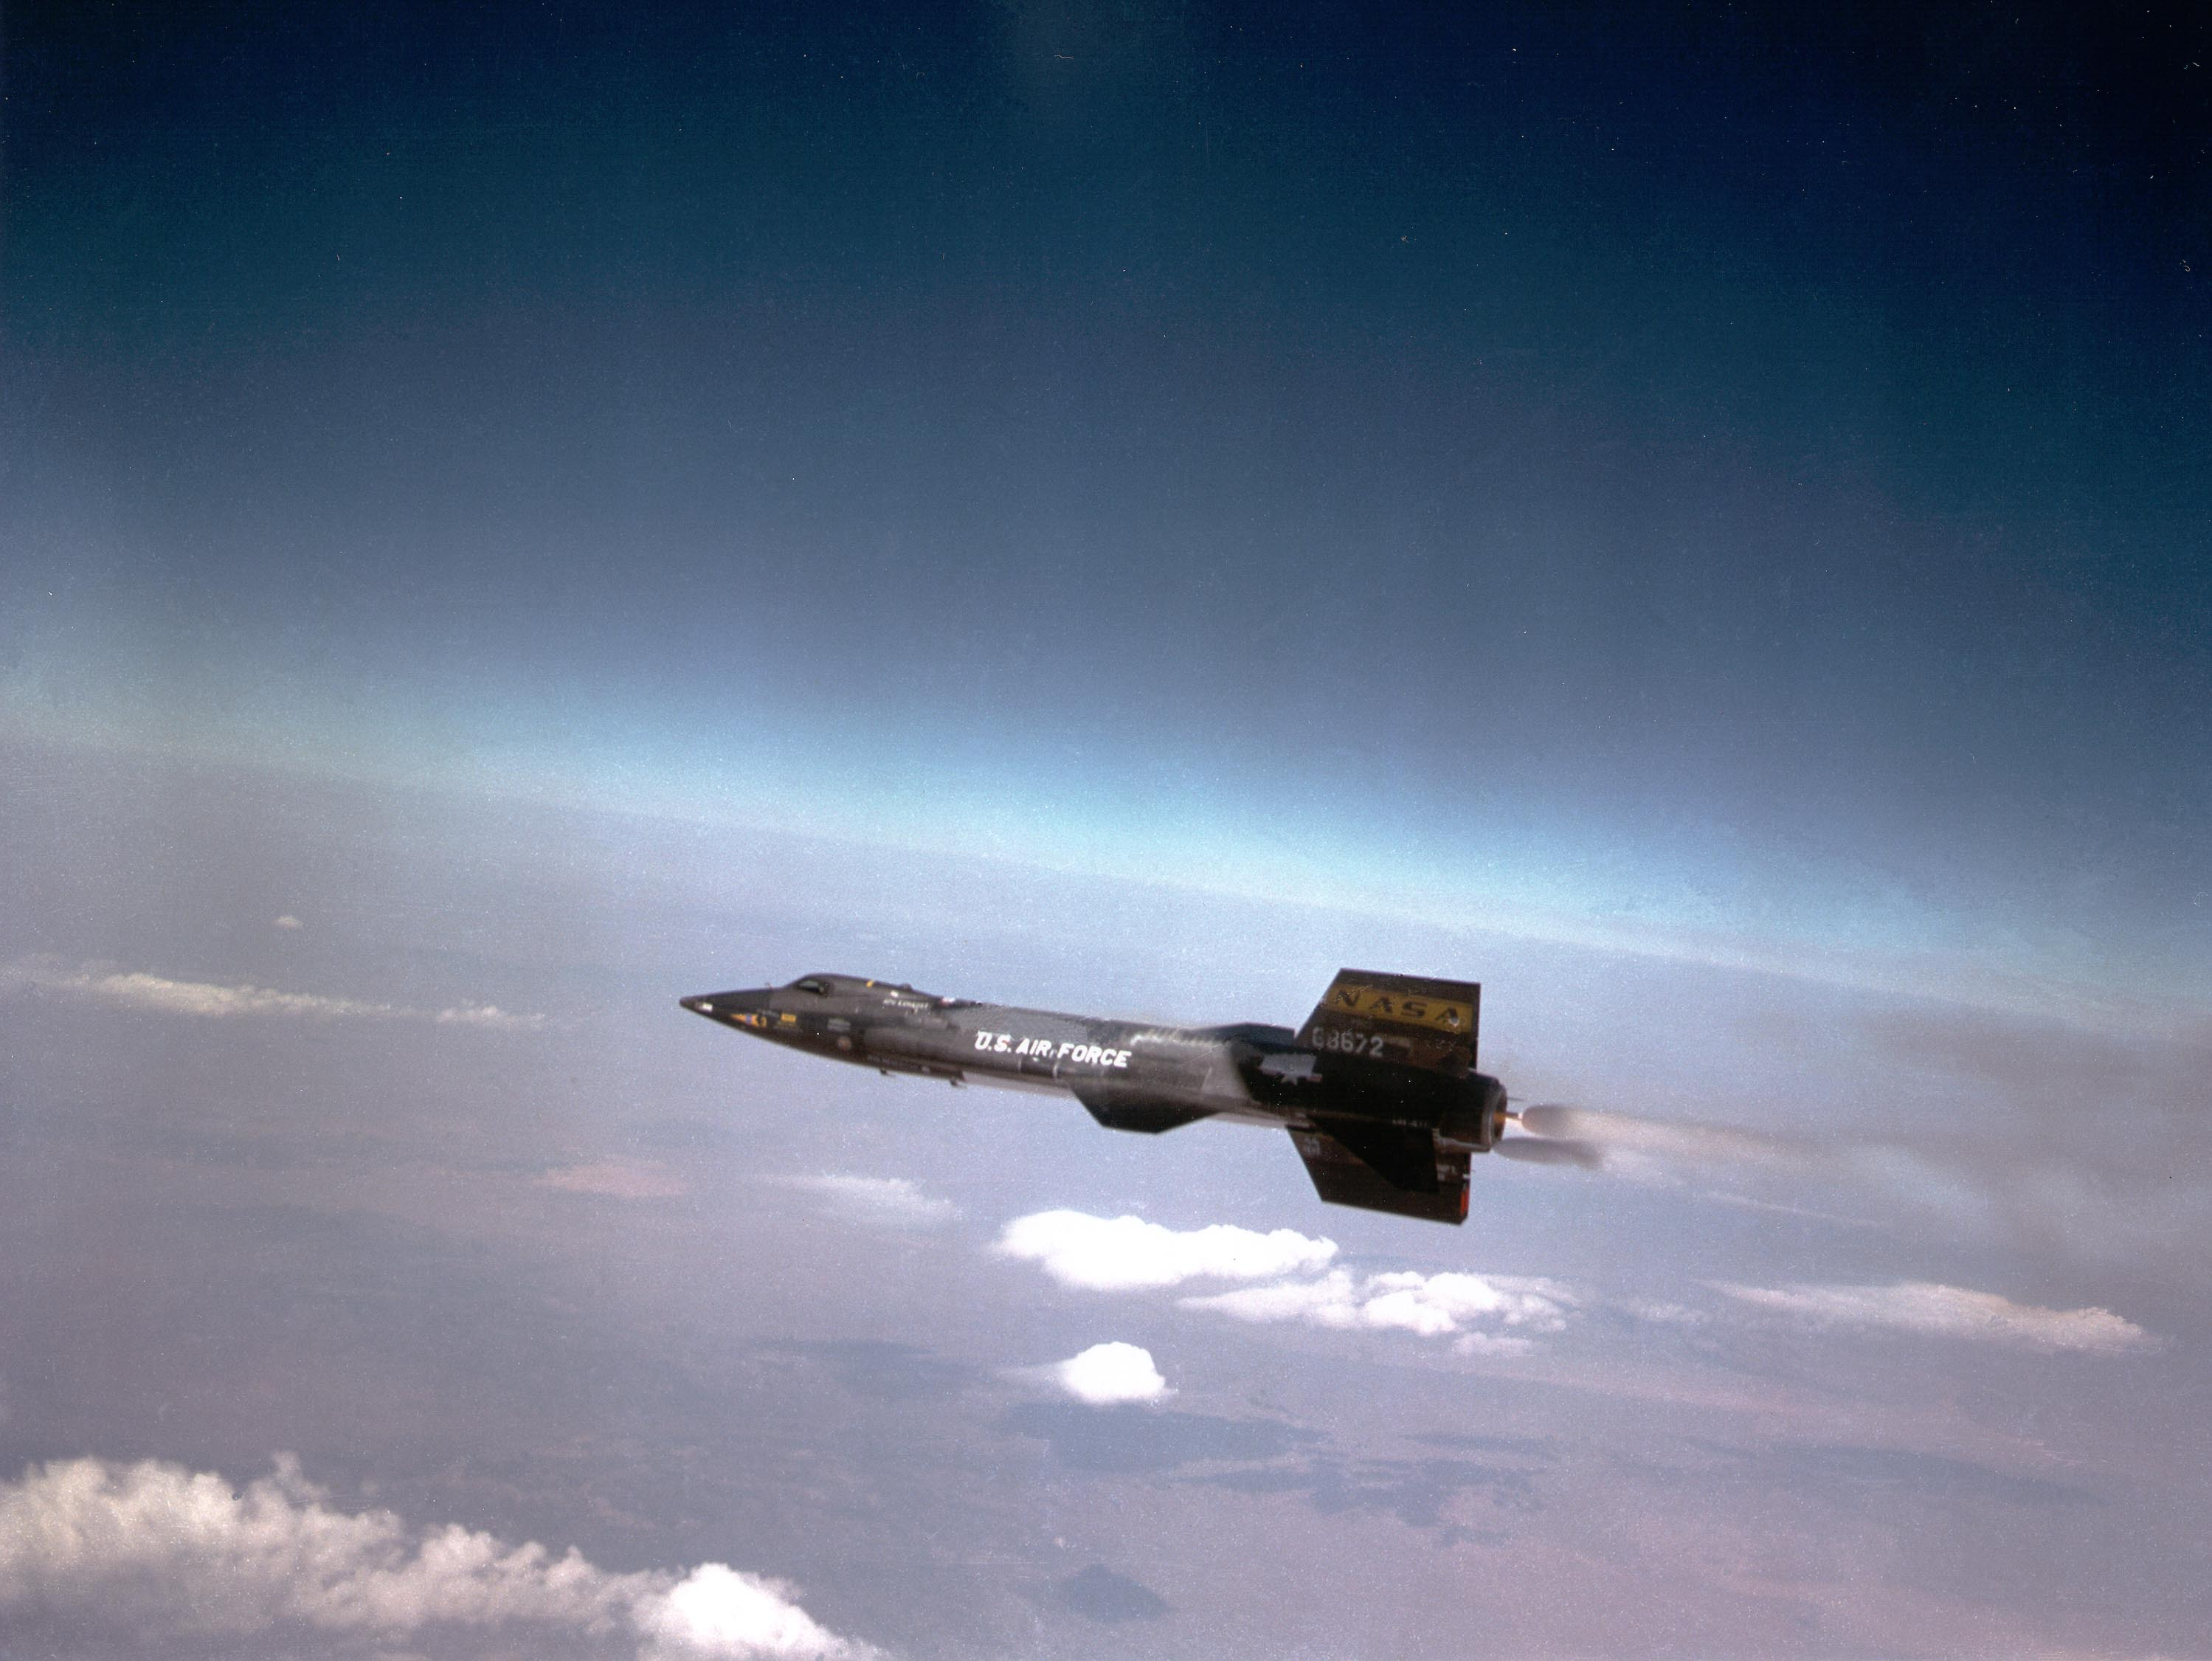
\includegraphics[width=3.5in]{\figurepath/x15flying.jpg}
    \caption{North American X-15 from Ref.\ \cite{x15picture}.\label{fig:x15flying}}
  \end{center}
\end{figure}

Toward the end of the X-15's career, there was a building interest in a new, advanced air-breathing propulsion system for hypersonic flight, as opposed to the rocket propulsion used on the X-15 and its predecessors.
This Hypersonic Research Engine (HRE) was to utilize concepts first disclosed by The Johns Hopkins Universities' Applied Physics Lab in 1959, as part of a project known as Supersonic Combustion Ramjet Missle (SCRAM).
The scramjet engines were initialy designed as pods, much like conventional turbofans on commercial and transport aircraft.
Early plans called for a podded scramjet to be fitted on the X-15, but it was quickly realized that this would not be possible.
To make scramjets practical for use in flight, the engine would have to be integrated intimately with the airframe, using the fore and aft sections of the vehicle as part of the inlet and nozzle of the scramjet.
Development of scramjet technology was pushed forward in the early 1980s in part by the U.S. Air Force, in order to develop a single-stage-to-orbit vehicle to deliver military weapons systems to space.
This ultimately led to the National Aero-Space Plane (NASP) program, and the design of the 160 foot long Rockwell X-30.
This program lasted over ten years and lead to many advances in scramjet propulsion research and the study of flexible hypersonic vehicles, but none of these vehicles were ever built.

\begin{figure}[h]
  \begin{center}
    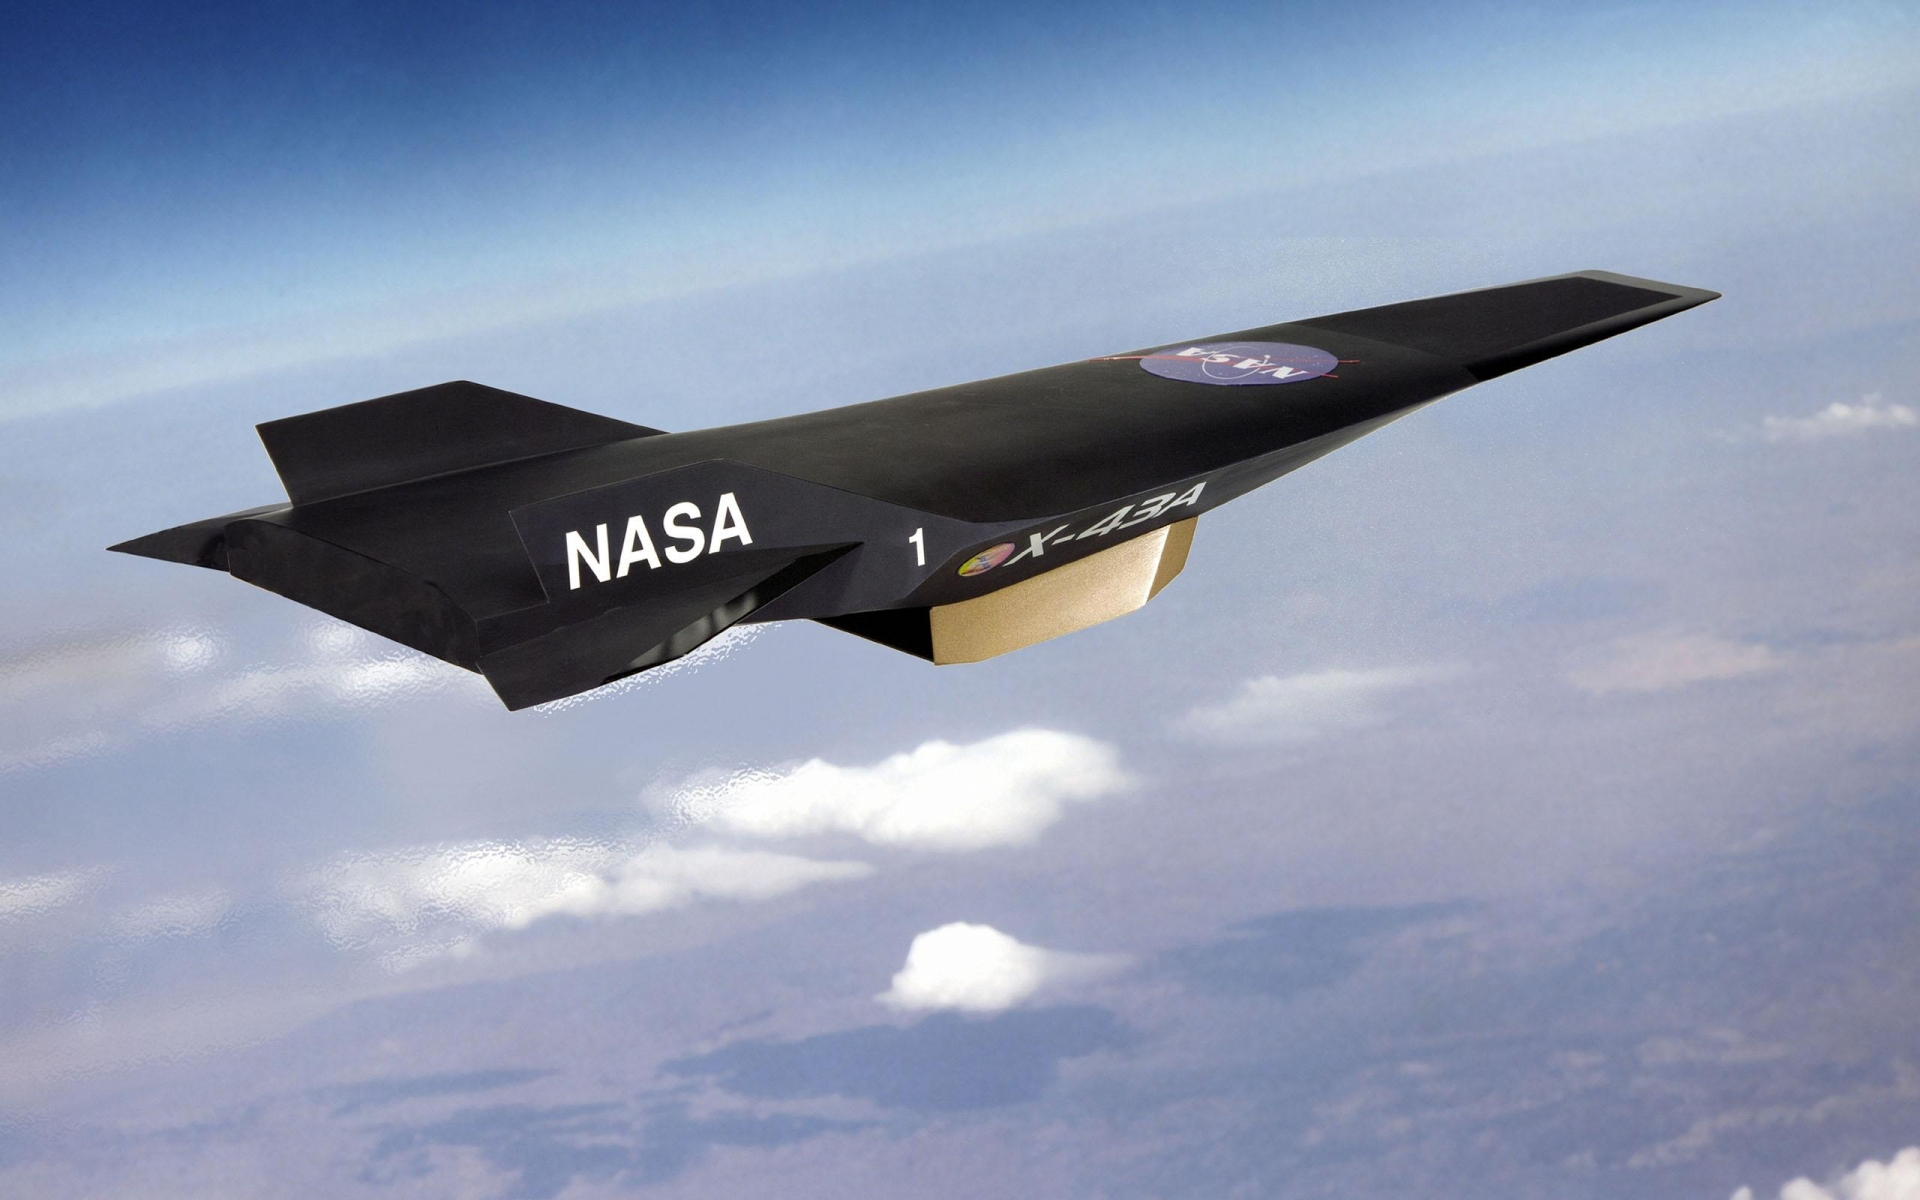
\includegraphics[width=3.5in]{\figurepath/nasa_x43.jpg}
    \caption{NASA X-43A from Ref.\ \cite{x43picture}.}
  \end{center}
\end{figure}

Hypersonic research slowed for some years, until scramjet research emerged again in the early 1990s as part of a collaboration between the United States and Russia.
This collaboration saw scramjets mounted aboard rockets being tested in flight.
Control again became a critical challenge in hypersonic flight, this time in the control of the engines.
Fuel delivery had to be controlled precisely to keep the engines operating in supersonic combustion mode, and avoid a condition known as unstart.
Control systems aboard these rocket-mounted scramjets were designed to monitor pressures within the engines and adjust fuel flow to prevent unstart, but the early control systems were not yet ready for this demanding challenges.
An all-American effort at practical scramjet powered hypersonic flight was born in 1996 under the name Hyper-X\ \cite{freeman.hyperx.1997}.
Hyper-X was an eight year NASA program with the goal of demonstrating the viability of air-breathing hypersonic flight.
The demonstrator vehicle for this program, the X-43, was 12 feet long, and 5 feet wide.
The first flight took place in June 2001 and failed, but in March 2004 the X-43A became the first vehicle to ever be propelled during hypersonic flight by an air-breathing engine, reaching a speed of Mach 6.8 for 11 seconds.
The third flight in November 2004 lasted 10 seconds and reached a speed of Mach 9.6.
These ground breaking flights demonstrated the practicability of a scramjet powered hypersonic vehicle, and are alongside the X-15 in terms of importance in the history of hypersonic flight.

In the 1990s and 2000s, many hypersonics programs have been introduced, including HyTECH, HyShot, HyCause, HIFiRE, and more.
The most notable platform since the X-43A was the X-51, built by Boeing and managed by the U.S. Air Force Research Lab (AFRL).
While the X-43A demonstrated the feasibility of scramjet powered flight, a new record was set by the X-51 in 2010 by maintaining scramjet powered flight at Mach 5 for 140 seconds.
The second X-51 flight took place in 2011 and ended early due to unstart, and during the third test flight the X-51 lost control and fell into the ocean.
History was made once again in May 2013, when the X-51 made the longest air-breathing hypersonic flight, maintaining Mach 5.1 for 240 seconds under its own power.

\begin{figure}[h]
  \begin{center}
    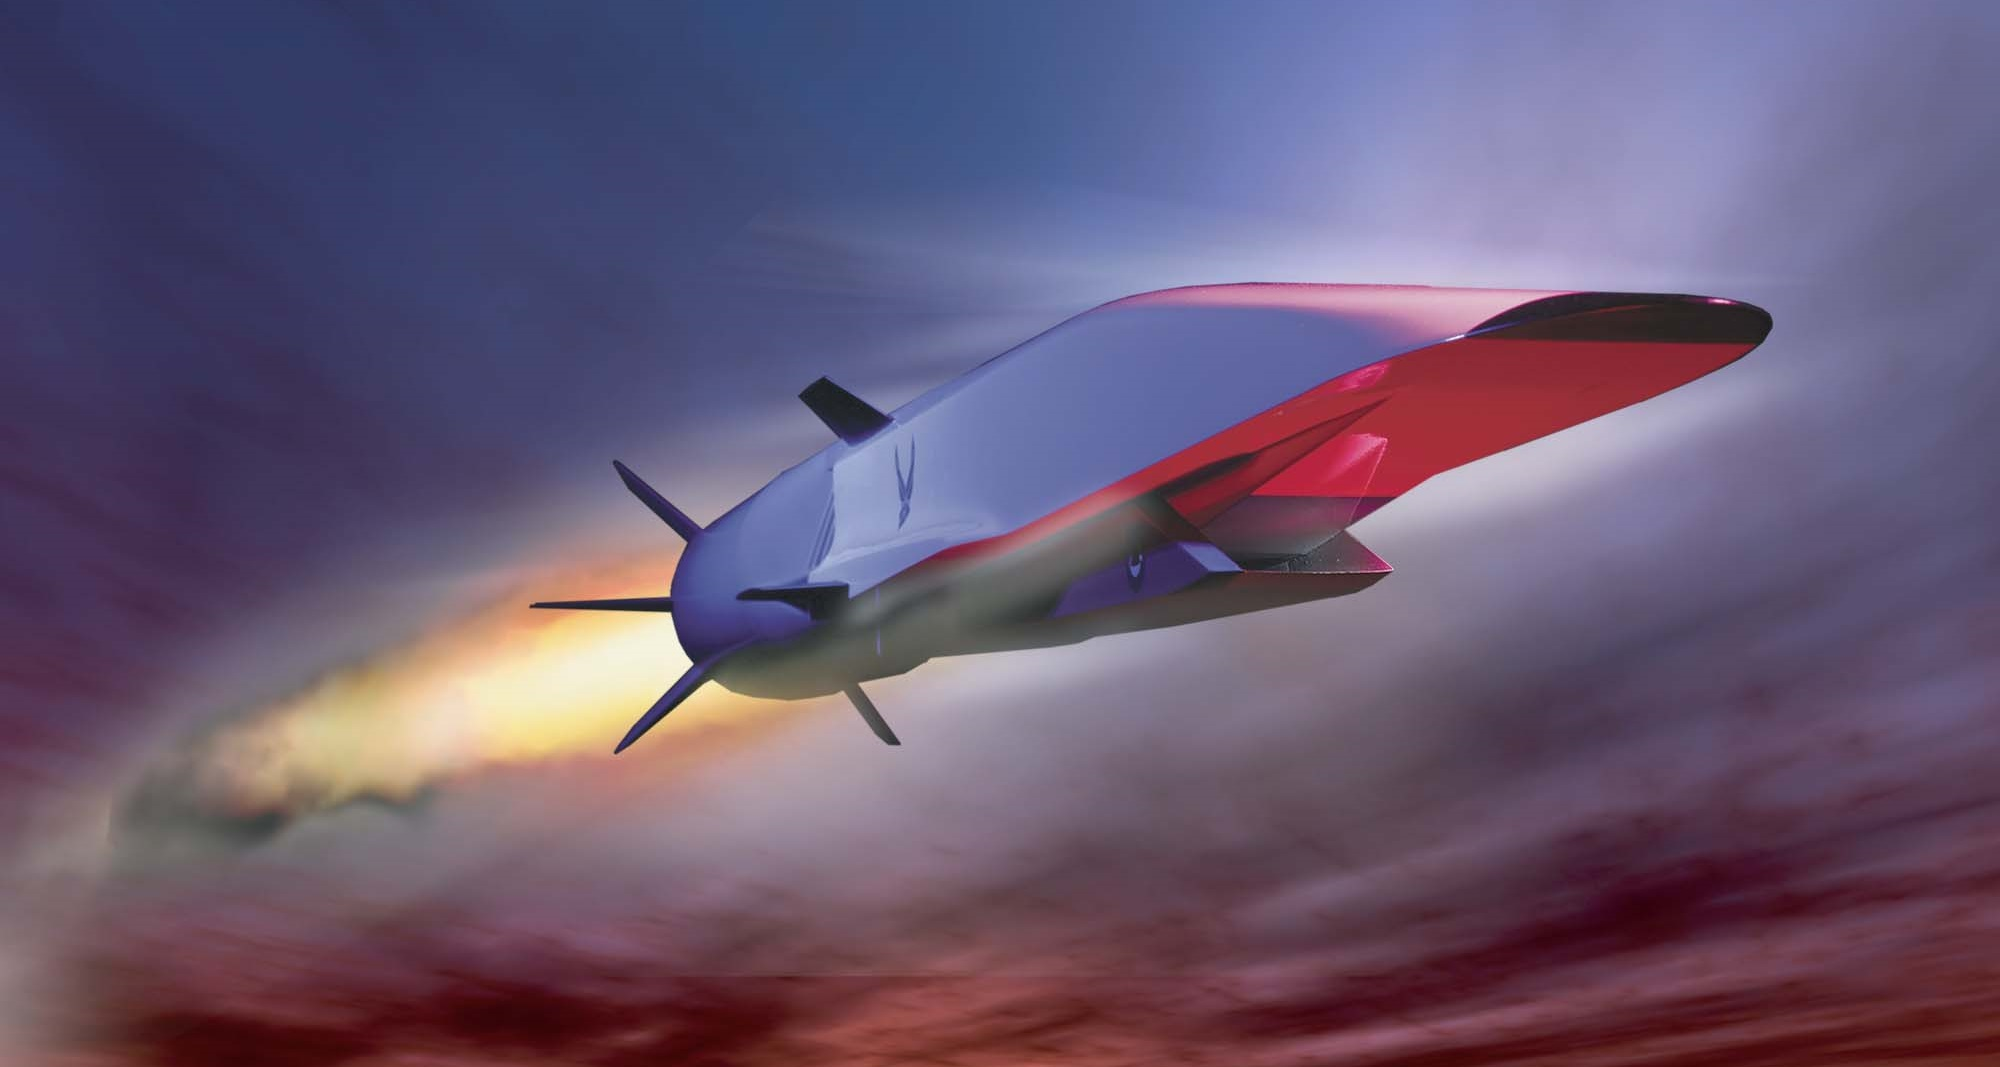
\includegraphics[width=3.5in]{\figurepath/boeing_x51_v3.jpg}
    \caption{Boeing X-51 waverider from Ref.\ \cite{x51picture}.}
  \end{center}
\end{figure}

The history of hypersonic flight is still in the making, with current research centered around the sustained flight of air-breathing vehicles.
The previous trajectories flown by aircraft such as the X-15, X-43 and X-51 were fairly benign in that abrupt and sudden maneuvers were generally avoided, and the goal was to demonstrate primarily the ability of these experimental aircraft to maintain hypersonic flight under their own power.
As technology grows the demands of these vehicles will grow too.
Current research is being performed to develop new materials and engine designs for these vehicles, as well as advanced control systems which will allow complex maneuvers to be performed while maintaining stability even in situations where unstart conditions are encountered.
One project in particular is the HIFiRE program, which is a collaboration between the U.S. Air Force Research Laboratory and the Defence Science Technology Organisation in Australia.
In particular, the HIFiRE 6 flight vehicle shown in Figure~\ref{fig.hifire6vehicle} is designed to evaluate the tracking performance of an adaptive flight control system on a representative hypersonic vehicle that is executing a set of predefined maneuvers\ \cite{adamczak.hifire6.2015, bolender.hifire6.2012, dauby.hifire6overview.2015}.

\begin{figure}[H]
  \begin{center}
    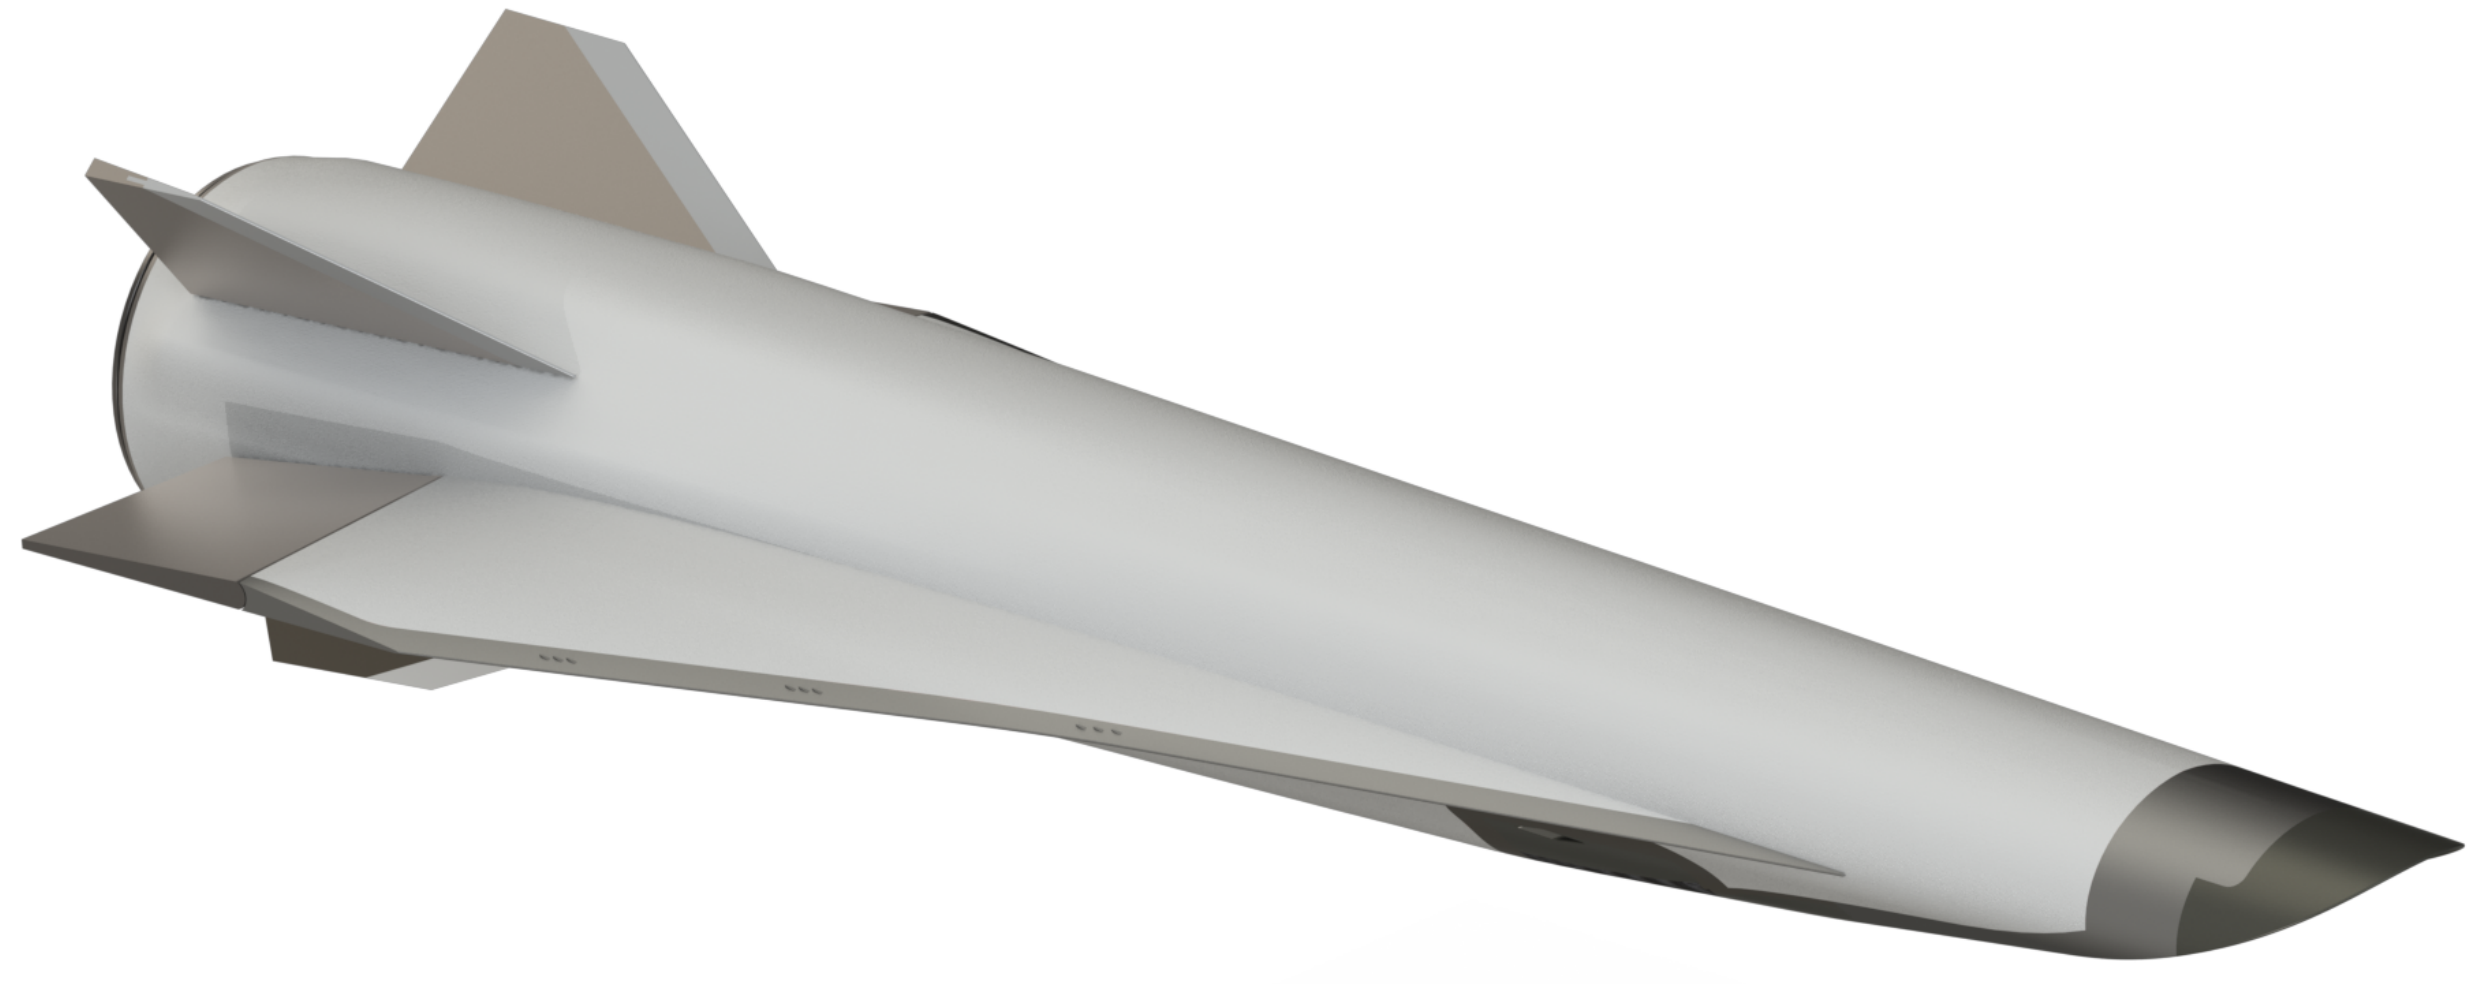
\includegraphics[width=3.5in]{\figurepath/hifire6.png}
    \caption{HIFiRE 6 flight vehicle from Ref.\ \cite{dauby.hifire6overview.2015}.\label{fig.hifire6vehicle}}
  \end{center}
\end{figure}

\subsection{Control of Hypersonic Vehicles}

The equations of motion which describe an aircraft are nonlinear, but in most cases it is acceptable to linearize these equations to facilitate control design and analysis.
This led to the description of aircraft dynamics using the transfer function, and to simple stability augmentation systems such as roll and yaw dampers\ \cite{cook.flightdynamics.2007}.
These flight control systems were simple, low-order, linear dynamic feedback compensators such as lead-lag and PID, and typically used small feedback gains\ \cite{dazzo.linearcontrol.2003, mclean.flightcontrol.1990, yechout.flightmechanics.2003}.
Thorough frequency domain analysis was critical to ensure a robust design.
Optimal control techniques slowly began seeing use in flight control in the early 1980s with limited success, but have now become more widely used\ \cite{abzug.stability.2005, chandler.lqrshortcomings.1983, stengel.flightdynamics.2004, stevenslewis.aircraftcontrol.2003}.
Many robust, nonlinear, and adaptive control solutions are proposed in recent literature\ \cite{bolender.hifire6.2012, gibson.adaptive.2008, huang.robust.2012, hughes.hinfinity.2010,   rollins.nonlinear.2013, xu.adaptive.2004} which include sliding mode, H$_{2}$/H$_{\infty}$, dynamic inversion, and neural network control, as well as many other techniques.

\section{Hypersonic Vehicle Modeling}

The Generic Hypersonic Vehicle (GHV) which is used as a platform for analysis and control design is shown in Figure~\ref{fig.ghvclouds}.
The GHV is a small, pilotless, blended wing-body vehicle, with 3-D inlet and nozzle, and axisymmetric through-flow scramjet engine.
There are four aerodynamic control surfaces which can be moved independently, consisting of two elevons and two rudders.
The relevant vehicle properties are listed in Table~\ref{tab:vehicle_properties}.

\begin{figure}[h]
  \begin{center}
    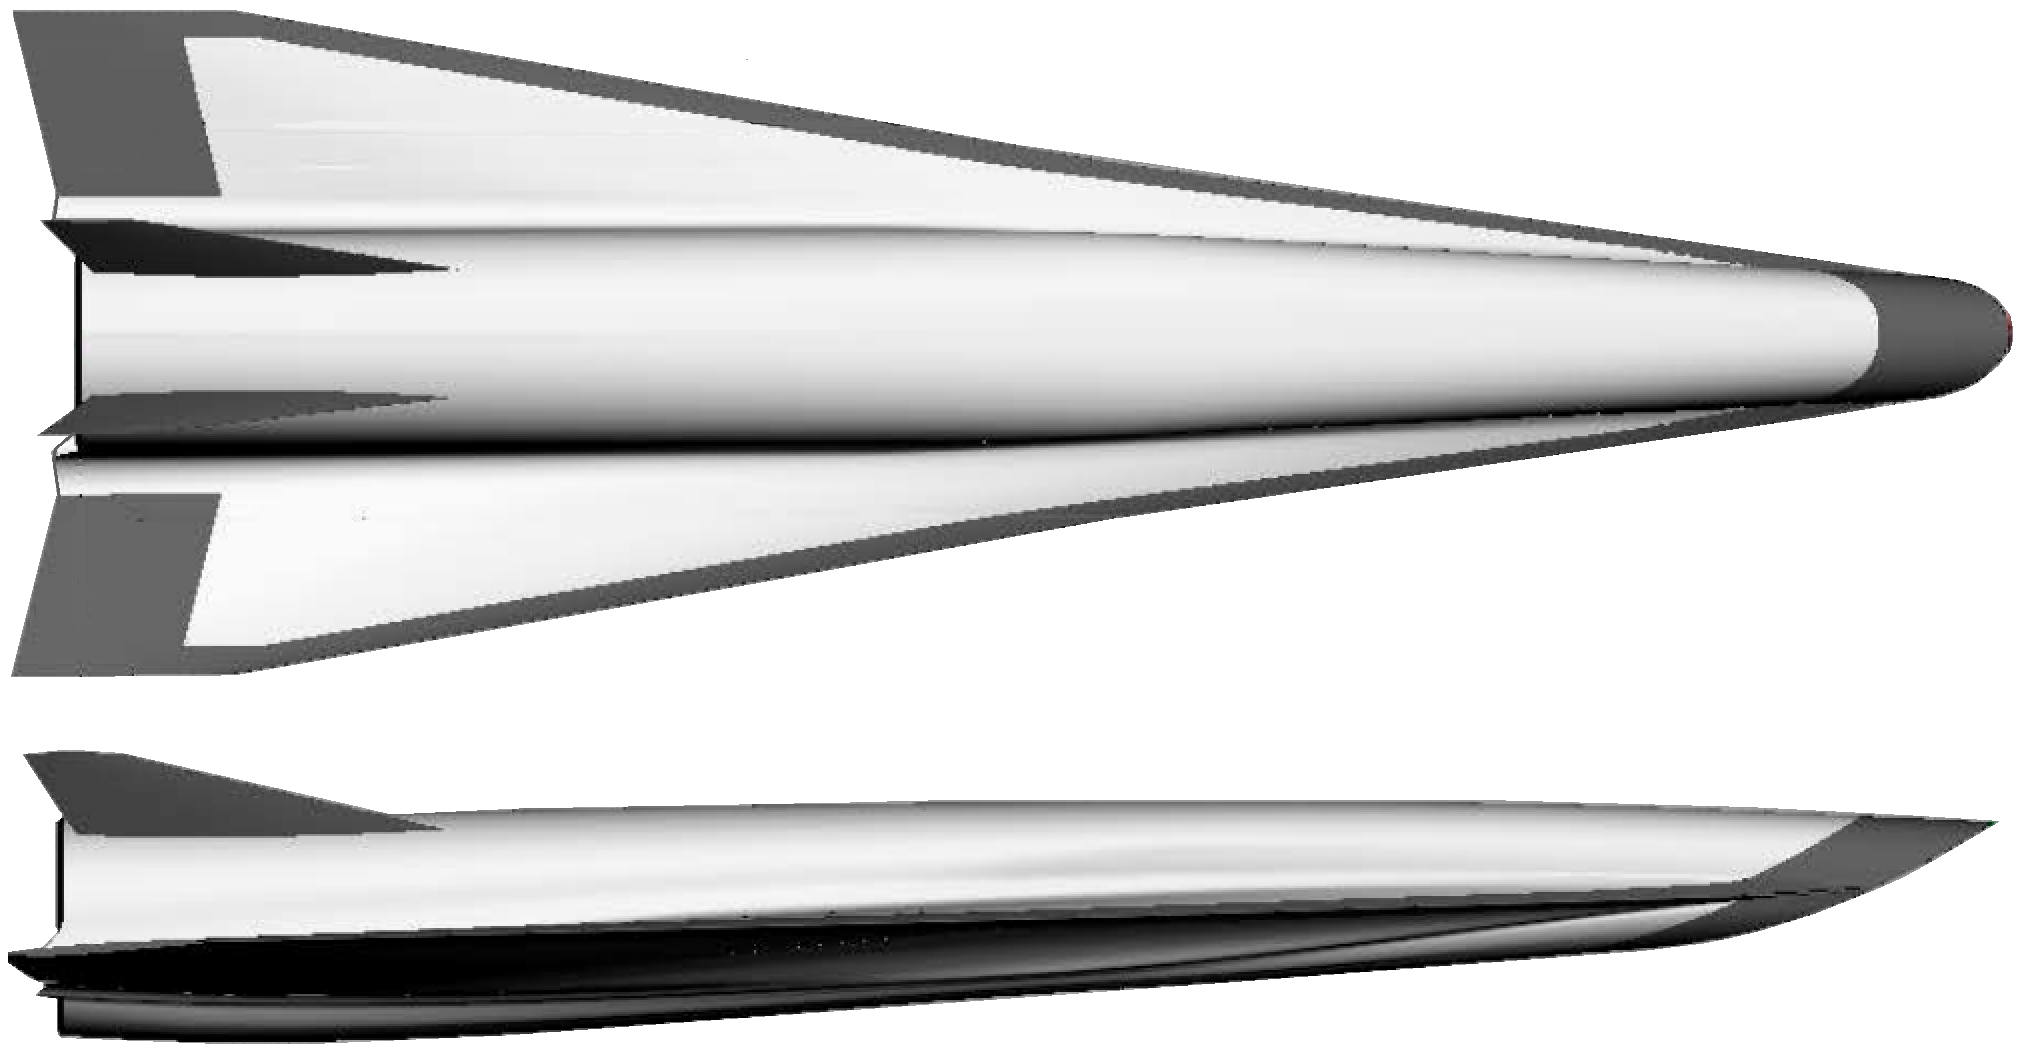
\includegraphics[width=4.5in]{\figurepath/ghvmodelview4.png}
    \caption{AFRL Generic Hypersonic Vehicle from Ref.\ \cite{ruttle.ghv.2012}.\label{fig.ghvclouds}}
  \end{center}
\end{figure}

The GHV was developed by the Air Force Research Lab in an effort to create a publicly releasable hypersonic vehicle model for studies of operability, controllability, and aero-propulsion integration as described in Reference\ \cite{ruttle.ghv.2012}.
The objective was to design a common vehicle which would be relevant to the technical efforts of current hypersonic projects, including the HIFiRE 6 vehicle, which the GHV closely resembles, as can be seen in Reference\ \cite{bolender.hifire6.2012}.
This GHV was designed be launched on rocket to accelerate to cruise at Mach 6, at a dynamic pressure of between 1000--2000 lb/ft$^{2}$.
The mission profile for the GHV then required maneuvers to be performed during the middle of the cruise phase before descending and decelerating, and making an unpowered maneuver to evaluate the potential to make a controlled landing.
The GHV has the capability to perform sustained maneuvers up to a load factor of up to approximately 2G.

\begin{table}[H]
  \centering
  \caption{Vehicle properties}
  \begin{tabular}{llr}
    \toprule
    Parameter & Unit & Value \\ \midrule
    Gross weight & [lbm] & $1220.3$ \\
    Empty weight & [lbm] & $993.3$ \\
    Vehicle length & [in] & $175.9$ \\
    Span & [in] & $58.6$ \\
    Nose diameter & [in] & $11.0$ \\
    Tail diameter & [in] & $18.8$ \\
    \bottomrule
  \end{tabular}\label{tab:vehicle_properties}
\end{table}

The aerodynamic data for the GHV was calculated using Hypersonic Engineering Aerothermodynamic Trajectory Tool Kit (HEAT-TK), developed for the Air Force by Boeing\ \cite{carter.heattk.2005}, and the engine data is calculated using the Ramjet Performance Analysis (RJPA) code, developed at Johns Hopkins University's Applied Physics Lab.

The equations of motion describing many aircraft can be derived assuming a flat, non-rotating Earth.
Due to the high flight speed of a hypersonic vehicle in the atmosphere, the rotation and curvature of the Earth are typically significant, and should not be neglected.
Thus, the governing equations of motion for the GHV are derived assuming the vehicle is a rigid body flying through the atmosphere of a spherical, rotating Earth.
The equations of motion describing the GHV are given in References\ \cite{billamoria.eom.1995, etkin.atmosphericflight.1972}, and will be presented in this chapter for completeness.

\subsubsection{Notation}
In deriving and applying the equations of motion which govern the motion of an aircraft, care must be taken to carefully book-keep the various vector quantities which describe the position, velocity and orientation of the aircraft.
For instance, when considering the velocity of an aircraft, it must be kept clear both with which frame the velocity is with respect to, and in which frame the velocity vector is described.
Some of the standard notation describing the expression of vectors in various reference frames is outlined below.
\begin{itemize}
  \item{$f_{a}$ denotes reference frame $a$.}
  \item{$O_{a}$ denotes the origin of reference frame $a$.}
  \item{$V^{a}_{b}$ describes the velocity of the origin of reference frame $b$ relative to the axes of reference frame $a$, described using the coordinate system of reference frame $b$.}
  \item{$\omega^{a,b}_{c}$ describes the angular velocity of reference frame $a$ relative to reference frame $b$ described using the axes of reference frame $c$. Omission of the second superscript implies the angular velocity of coordinate system $a$ is with respect to inertial axes. When the subscript is omitted, it is implied this quantity is described in the coordinates of frame $a$. For example $\omega^{B}$ is the inertial angular velocity of frame $f_{B}$, described using the axes of frame $f_{B}$.}
  \item{The transformation $R_{ab}$ describes a vector transformation from being expressed in reference frame $b$ to being expressed in reference frame $a$.}
  \item{$\frac{dV_{a}}{dt}\bigr|_{b}$ denotes the rate of change of $V_{a}$ with respect to frame $b$.}
  \item{All vectors are describing a relation of frame $a$ to frame $b$ are described along the axes of frame $a$.}
\end{itemize}

In many cases, the equations of motion can be greatly simplified when studying the dynamics of an aircraft.
Such simplifications often center around assuming the Earth is flat, but this may be an oversimplification for problems of hypersonic atmospheric flight.
While this simplification still might be acceptable for calculations involving the attitude dynamics where the rotating earth terms are typically very small, in trajectory calculations the rotating earth terms for a hypersonic vehicle become non-negligible.
This section presents the equations of motion that describe the GHV.\@

\subsection{Equations of Motion}

The equations of motion are developed using an Earth-centered, Earth-frame $f_{EC}$ with origin at the center of a spherical, rotating Earth.
It is assumed that the atmosphere travels uniformly with Earth as it rotates with angular velocity $\omega_{\text{earth}}$ in inertial space, and that the aircraft is sufficiently rigid that flexible structural effects can be neglected.
The position of the GHV around Earth and relative to $f_{EC}$ is described by its latitude $\lambda$, longitude $\tau$, and distance from the center of the Earth, $\mathscr{R}$.
These three coordinates give the location of the vehicle-carried frame $f_{V}$, defined with $z$-axis always pointing toward the origin of $f_{EC}$.

\begin{figure}[H]
  \begin{center}
    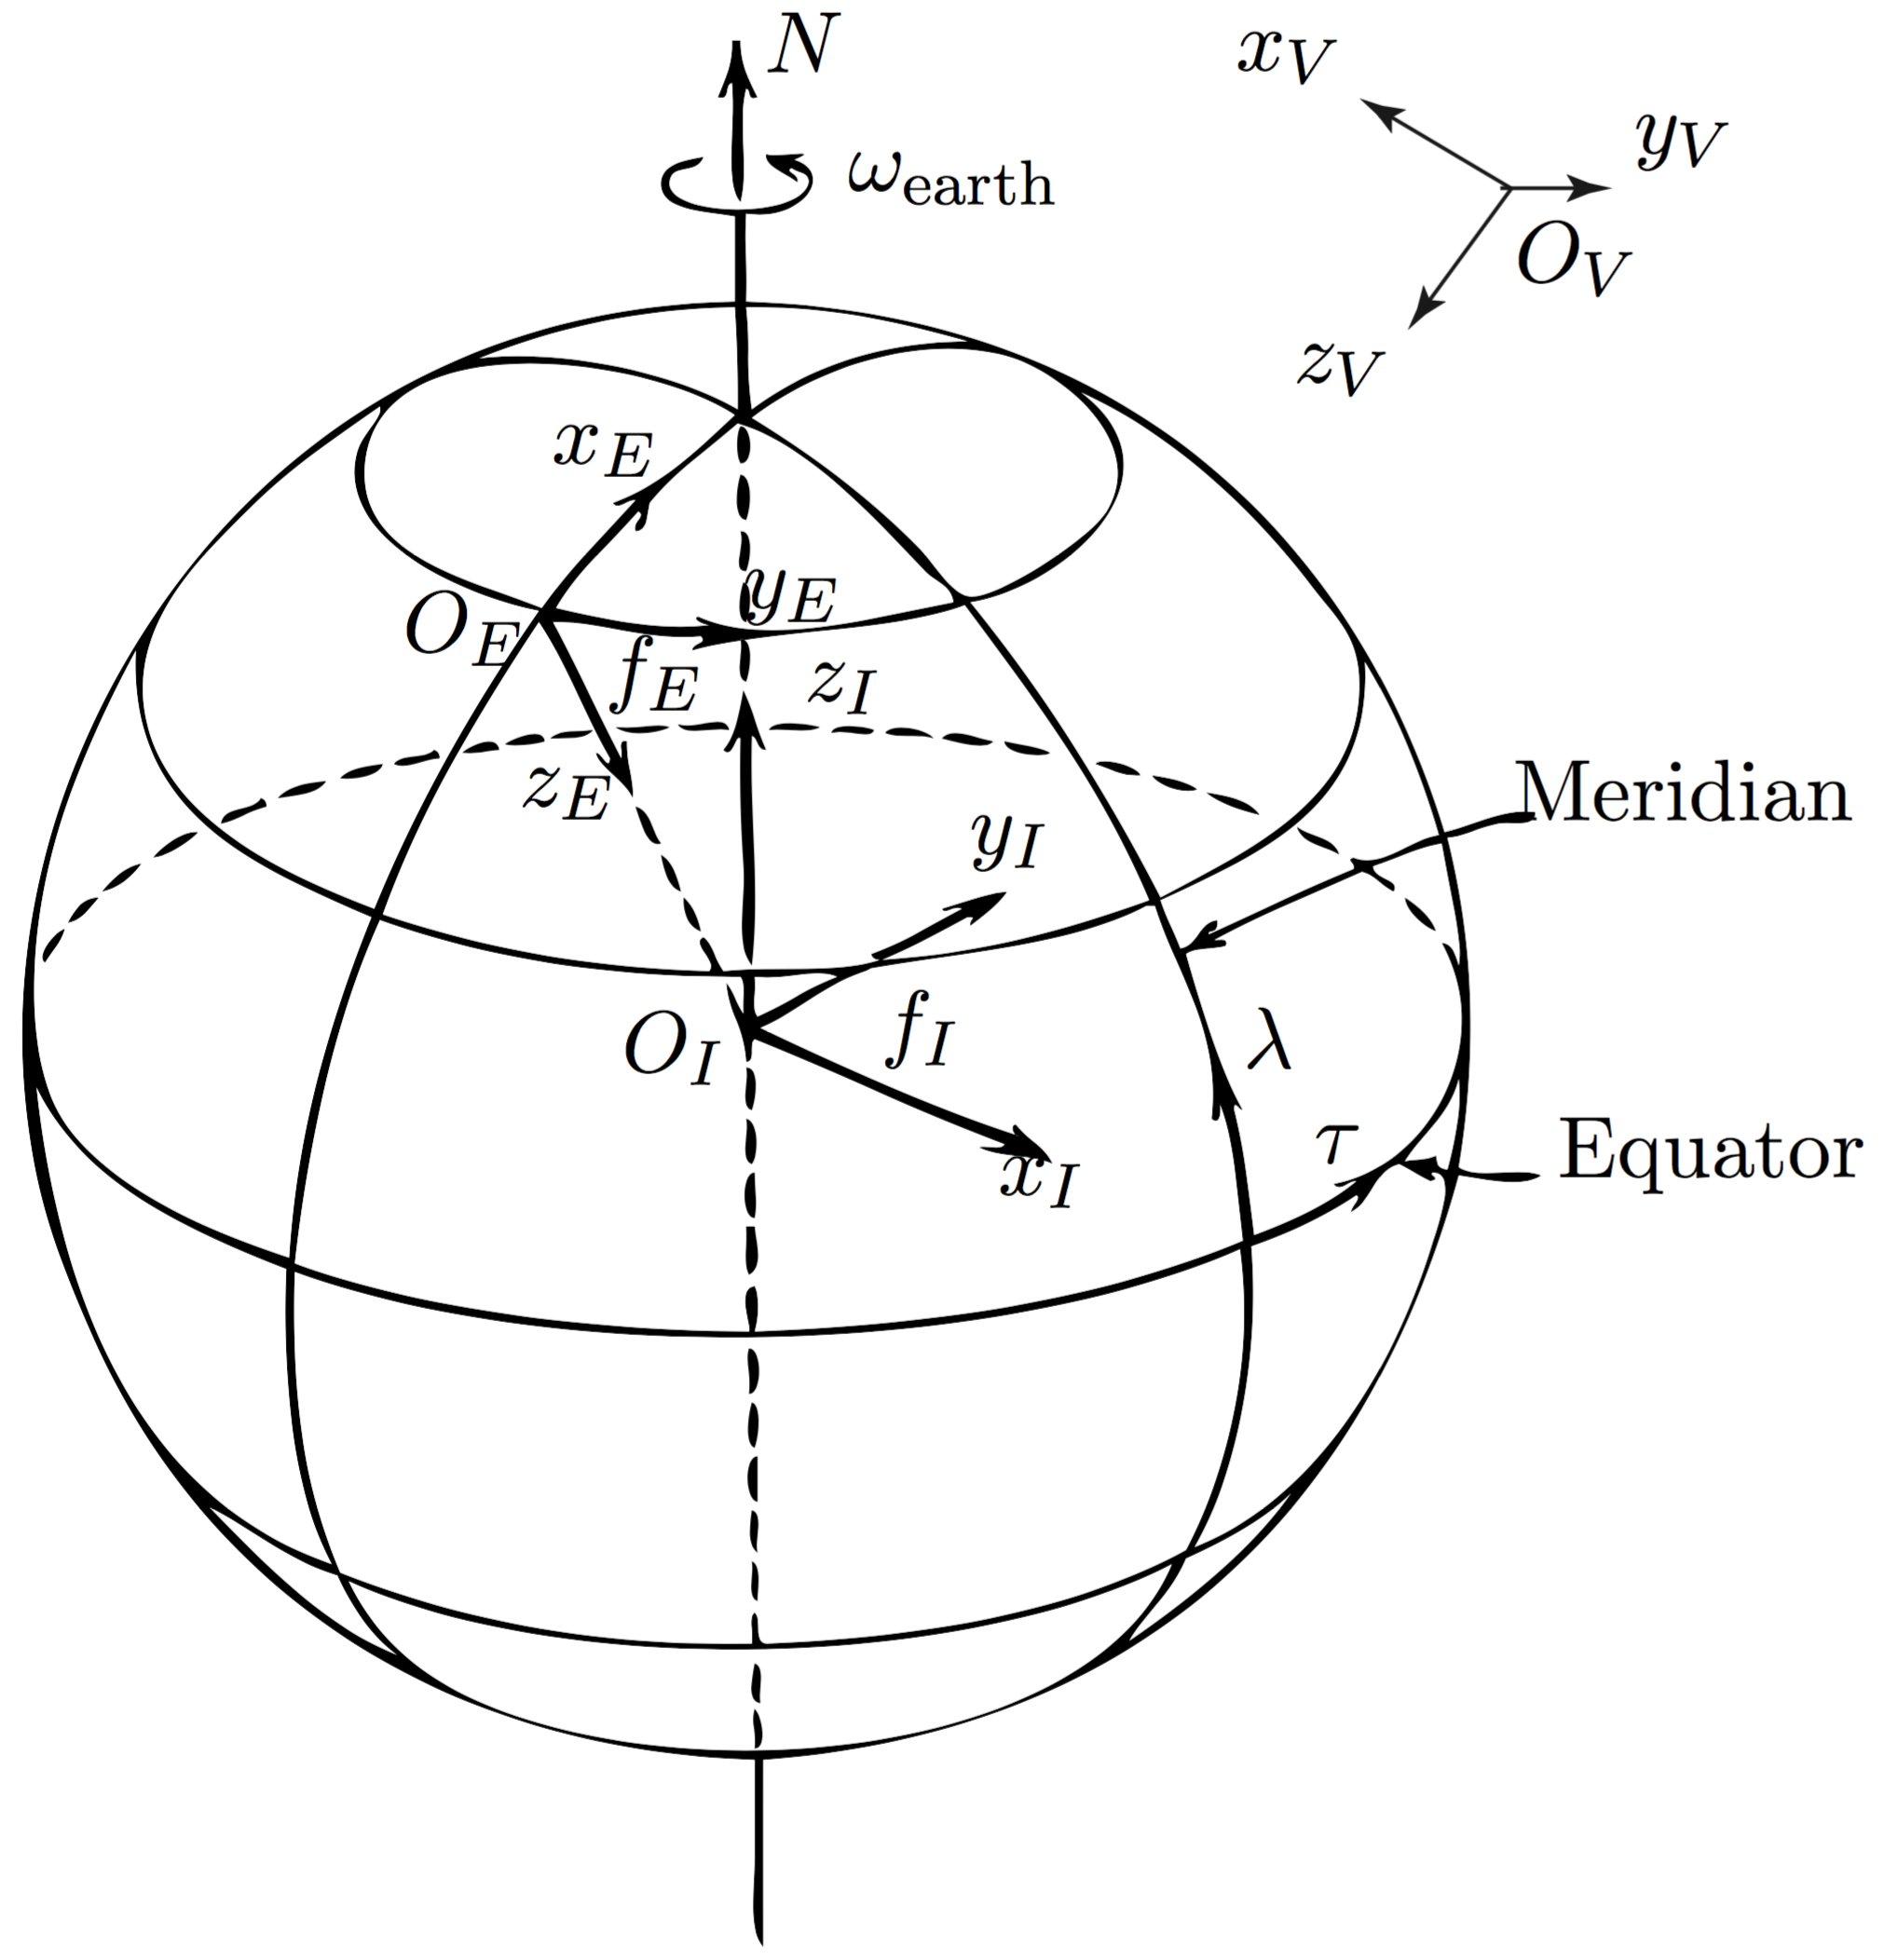
\includegraphics[height=2.5in]{\figurepath/globe_fig.png}
    \caption{Reference frames\ \cite{etkin.atmosphericflight.1972}\label{globe_fig}}
  \end{center}
\end{figure}

The vehicle carrying frame $f_{V}$ is a frame with origin attached to vehicle at the CG, and the z-axis $O_{V}z_{V}$ is defined to point vertically downward along the local $g$ vector.
$O_{V}x_{V}$ is defined to point north, and $O_{V}y_{V}$ east as shown in Figure~\ref{globe_fig}.
The vehicle-carried frame has angular velocity $\omega^{V}$ due to the curvature of the earth.
The body-fixed reference frame $f_{B}$ is a right-handed coordinate system attached to the GHV with $x$-axis pointing towards the nose of the aircraft along the longitudinal axis, and the $z$-axis pointing down.
This body-fixed axis system is used to derive the equations of motion for the GHV.\@

In deriving the equations of motion, the only additional assumption is that the centripetal acceleration due to $\omega_{\text{earth}}$ is negligible.
The equations of motion describe the dynamics of the GHV around the Earth when subject to external forces and moments.
These forces and moments, given in the body axes by $F_{B}$, and $M_{B}$ respectively, are due to the thrust and aerodynamic forces acting on the GHV, and are taken from pre-determined look-up tables within the simulation.
The aerodynamic forces depend on on control surface deflection angle, dynamic pressure, angle of attack, and sideslip angle.
The thrust forces depend on on control surface deflection angle, dynamic pressure, and angle of attack.

\subsubsection{Force Equations}

The force equation describing the the motion of the GHV center of gravity in body axes is given as the following
\begin{equation}
  \label{eqn.forceEqn}
  \frac{dV^{A}_{B}}{dt}\biggr|_{B}+\omega^{B}\times V^{A}_{B}+
  \omega^{E}_{B}\times V^{A}_{B}+\omega^{E}_{B}\times(\omega^{E}_{B}\times\mathscr{R})
  =
  g+(F_{A}+F_{T})/m
\end{equation}
where $V^{A}_{B}$ denotes the velocity of $f_{B}$ relative to the atmosphere-fixed reference frame, and $\omega^{E}_{B}$ is the inertial angular velocity of the Earth-fixed frame $f_{E}$, described using the coordinate system of the body reference frame.
Note in this work that the atmosphere is assumed fixed with respect to the earth, so $f_{A}=f_{E}$.
The components of the atmospheric velocity are
\begin{equation*}
  V_{B}^{A}=
  \bigr[
  \begin{array}{ccc}
    u & v & w
  \end{array}\bigr]^{\top}
\end{equation*}
The force vector $F_{B}$ that represents all non-gravitational forces acting on the body in body axes is given by
\begin{equation*}
  F_{B}=
  \bigr[
  \begin{array}{ccc}
    X & Y & Z
  \end{array}\bigr]^{\top}
\end{equation*}
In the Equation (\ref{eqn.forceEqn}) this force is separated into aerodynamic and propulsive contributions as $F_{B}=F_{A}+F_{T}$ where the aerodynamic and propulsive forces have components given by
\begin{equation}
  \label{eqn.AeroAndPropulsiveForces}
  \begin{split}
    F_{A}&=
    \bigr[
    \begin{array}{ccc}
      X_{A} & Y_{A} & Z_{A}
    \end{array}\bigr]^{\top} \\
    F_{T}&=
    \bigr[
    \begin{array}{ccc}
      X_{T} & Y_{T} & Z_{T}
    \end{array}\bigr]^{\top}
  \end{split}
\end{equation}

\subsubsection{Moment equations}

The vehicle moments are described by the following equation.
Note the absence of any rotor contributions to the vehicle moment, as the scramjet engine lacks moving parts, unlike jet-turbine powered craft.
\begin{equation}
  \label{eqn.momentEqn}
  J\frac{d\omega^{B}}{dt}\biggr|_{B}+\omega^{B}\times J\omega^{B}=M_{A}+M_{T}
\end{equation}
$\omega_{B}$ is the angular velocity of the body frame relative to the inertial frame, with the rate of change evaluated in the body frame, and components
\begin{equation*}
  \omega^{B}=
  \bigr[
  \begin{array}{ccc}
    p & q & r
  \end{array}\bigr]^{\top}
\end{equation*}
The total torque in body axes is given by
\begin{equation*}
  M_{B}=
  \bigr[
  \begin{array}{ccc}
    L & M & N
  \end{array}\bigr]^{\top}
\end{equation*}
This total moment is split into the contributions due to aerodynamic and propulsive moments in Equation (\ref{eqn.momentEqn}) as $M_{B}=M_{A}+M_{T}$ where the aerodynamic and propulsive moments have components given by
\begin{equation}
  \label{eqn.AeroAndPropulsiveMoments}
  \begin{split}
    M_{A}&=
    \bigr[
    \begin{array}{ccc}
      L_{A} & M_{A} & N_{A}
    \end{array}\bigr]^{\top} \\
    M_{T}&=
    \bigr[
    \begin{array}{ccc}
      L_{T} & M_{T} & N_{T}
    \end{array}\bigr]^{\top}
  \end{split}
\end{equation}
The moment of inertia matrix $J$ is given by
\begin{equation*}
  J=
  \begin{bmatrix}
    J_{xx} & -J_{xy} & -J_{xz} \\
    -J_{xy} & J_{yy} & -J_{yz} \\
    -J_{xz} & -J_{yz} & J_{zz}
  \end{bmatrix}
\end{equation*}
Without any simplification, expansion of the moment equations would become very cumbersome.
In general, aircraft are symmetric about the $x-z$ plane, mass is uniformly distributed, and the body coordinate system is oriented such that $J_{xy}=J_{yz}=0$.
This allows the moment of inertia matrix for the GHV to be simplified to
\begin{equation*}
  J=
  \begin{bmatrix}
    J_{xx} & 0 & -J_{xz} \\
    0 & J_{yy} & 0 \\
    -J_{xz} & 0 & J_{zz}
  \end{bmatrix}
\end{equation*}

\subsubsection{Orientation Equations}

The orientation, or kinematic equations describe the orientation of the aircraft body axes with respect to the vehicle carried frame.
The relationship between Euler rates and body angular velocities in the vehicle- carried frame is given by

\begin{equation}
  \label{eqn.bodyRatesToEulerRates}
  \left[
  \begin{array}{c}
    \dot{\phi} \\
    \dot{\theta} \\
    \dot{\psi}
  \end{array}\right]=
  \left[
  \begin{array}{ccc}
    1 & \tan(\theta)\sin(\phi) & \tan(\theta)\cos(\phi) \\
    0 & \cos(\phi) & -\sin(\phi) \\
    0 & \sin(\phi)/\cos(\theta) & \cos(\phi)/\cos(\theta)
  \end{array}\right]
  \left[
  \begin{array}{c}
    p_{v} \\
    q_{v} \\
    r_{v}
  \end{array}\right]
\end{equation}
where $\phi$, $\theta$, and $\psi$ are the roll, pitch, and yaw or heading angles, respectively, and are known as the Euer angles.
The components of angular velocities $p_{v}$, $q_{v}$, and $r_{v}$ are for the aircraft with body-fixed reference frame $f_{B}$ and are relative to the vehicle-carrying frame $f_{V}$.
These components of angular velocity are about the $x$, $y$, and $z$ body axes, respectively.
The relative angular velocities of the GHV are related to the vehicle absolute angular velocities by
\begin{equation*}
  \begin{bmatrix}
    p_{v} \\
    q_{v} \\
    r_{v}
  \end{bmatrix}=
  \begin{bmatrix}
    p \\
    q \\
    r
  \end{bmatrix}-R_{BV}
  \begin{bmatrix}
    (\omega_{\text{earth}}+\dot{\tau})\cos{\lambda} \\
    -\dot{\lambda} \\
    -(\omega_{\text{earth}}+\dot{\tau})\sin{\lambda}
  \end{bmatrix}
\end{equation*}
where $R_{BV}$ is the orthogonal rotation matrix given by
\begin{equation*}
  R_{BV}=
  \begin{bmatrix}
    \cos{\theta}\cos{\psi} & \cos{\theta}\sin{\psi} & -\sin{\theta} \\
    \sin{\phi}\sin{\theta}\cos{\psi}-\cos{\phi}\sin{\psi} &  \sin{\phi}\sin{\theta}\sin{\psi}+\cos{\phi}\cos{\psi} & \sin{\phi}\cos{\theta}\\
    \cos{\phi}\sin{\theta}\cos{\psi}+\sin{\phi}\sin{\psi} &  \cos{\phi}\sin{\theta}\sin{\psi}-\sin{\phi}\cos{\psi} & \cos{\phi}\cos{\theta}
  \end{bmatrix}
\end{equation*}

The reason for the distinction between relative and absolute angular rates in the above equations is due to the spherical Earth.
If a hypersonic vehicle was flying continuous circles around the world, the relative angular rates $p_{v}$, $q_{v}$, and $r_{v}$ would all be zero as the aircraft would be stationary relative to the vehicle carried frame.
However, the absolute angular rates $p$, $q$, and $r$ would be non-zero, as the vehicle carried frame would be rotating as it moved over the surface of the Earth.

\subsubsection{Navigation Equations}

The location, or navigation equations describe the location of the origin of the body fixed coordinate system with respect to the inertial axes.
The quantities describing this location are latitude, longitude, and altitude.
The navigation kinematic equation is given by
\begin{equation}
  \label{eqn.NavigationEqn}
  \begin{bmatrix}
    \dot{\lambda}\mathscr{R} \\
    \dot{\tau}\mathscr{R}\cos{\lambda} \\
    -\dot{\mathscr{R}}
  \end{bmatrix}=R_{VB}
  \begin{bmatrix}
    u \\
    v \\
    w
  \end{bmatrix}
\end{equation}
where $R_{VB}=R_{BV}^{-1}$.

\subsection{State Space Representation}

The aerodynamic and propulsive forces and moments in\ \eqref{eqn.AeroAndPropulsiveForces} and\ \eqref{eqn.AeroAndPropulsiveMoments}, respectively depend on the vehicle state and input.
With this, the equations of motion in\ \eqref{eqn.forceEqn},\ \eqref{eqn.momentEqn},\ \eqref{eqn.bodyRatesToEulerRates}, and\ \eqref{eqn.NavigationEqn} can be represented in state-space form as
\begin{equation}
  \label{eqn.nonlinearStateSpace}
  \dot{X}(t) = f\bigr({X}(t), U(t)\bigr)
\end{equation}
with state vector
\begin{equation}
  \label{eqn.fullstatevectorx}
  X=\left[
  \begin{array}{cccccccccccc}
    V_{T} &  \alpha & q &\theta & h & \beta &p & r & \phi &\psi &\lambda & \tau
  \end{array}\right]^{\top}
\end{equation}
where $V_{T}$ is the total velocity, $\alpha$ and $\beta$ are the angle of attack and sideslip angle, $\phi$, $\theta$, and $\psi$ are the roll, pitch, and yaw angles, $p$, $q$, and $r$ are the absolute angular velocity components, and $\lambda$, $\tau$, and $h$ are the latitude, longitude, and altitude, of the GHV, respectively.
The input vector is given by
\begin{equation}
  \label{eqn.fullcontrolvector}
  U=\left[
  \begin{array}{cccc}
    u_{\text{th}} & u_{\text{elv}} & u_{\text{ail}} & u_{\text{rud}}
  \end{array}\right]^{\top}
\end{equation}
where $u_{\text{th}}$, $u_{\text{elv}}$, $u_{\text{ail}}$, and $u_{\text{rud}}$ are the throttle, elevator, aileron, and rudder inputs, respectively.
The entries of the state vector are arranged so as to facilitate separation of the lateral and longitudinal equations of motion during control design.
The deflection of the elevons are accomplished through static mixing, combining differential and collective deflections from the aileron and elevator commands, respectively, while both rudders are actuated together using the single rudder input.
The control vector $U_{5}$ contains the deflections of the right and left elevons ($u_{r,\text{elv}}$, $u_{l,\text{elv}}$), rudders ($u_{r,\text{rud}}$, $u_{l,\text{rud}}$), and throttle as
\begin{equation*}
  U_{5}=
  \bigr[
  \begin{array}{ccccc}
    u_{\text{th}} & u_{r,\text{elv}} & u_{l,\text{elv}} & u_{r,\text{rud}}  & u_{l,\text{rud}}
  \end{array}\bigr]^{\top}
\end{equation*}
The control allocation matrix $M$ is the matrix which defines the following transformation between control vectors $U_{5}$ and $U$ as
\begin{equation*}
  U = MU_{5}
\end{equation*}
where control allocation matrix is
\begin{equation*}
  M=
  \left[
  \begin{array}{ccccc}
    1 & 0 & 0 & 0 & 0 \\
    0 & 1/2 & 1/2 & 0 & 0 \\
    0 & 1/2 & -1/2 & 0 & 0 \\
    0 & 0 & 0 & 1/2 & 1/2 \\
  \end{array}\right]
\end{equation*}


\section{Open-Loop Analysis}

The open-loop behavior of the GHV was analyzed about a nominal flight condition of $M=6$, $h=80,000$ ft, corresponding to a dynamic pressure of 1,474 lb/ft$^2$.
The geographical coordinates and heading of the GHV are insignificant in the equations of motion for the purposes of inner-loop control law development, and these state variables are dropped from the state vector (\ref{eqn.fullstatevectorx}) for trim, linearization, and control.
\begin{equation}
  \label{eqn.truncstatevectorx}
  X=\bigr[
  \begin{array}{ccccccccc}
    V_{T} &  \alpha & q &\theta & h & \beta &p & r & \phi
  \end{array}\bigr]^{\top}
\end{equation}
The state $X$ from this point forward is used to mean the truncated state (\ref{eqn.truncstatevectorx}), as it contains the primary quantities describing the vehicle dynamics that are to be controlled.

\subsection{Linearization}

The dynamics of the system with truncated state are described by\ \eqref{eqn.nonlinearStateSpace}.
The equilibrium, or trim state $X_{\text{eq}}$ and input $U_{\text{eq}}$ satisfy
\begin{equation}
  \label{eqn.eqptdef}
  \dot{X}_{\text{eq}}=f({X}_{\text{eq}},U_{\text{eq}})=0
\end{equation}
The equilibrium state and input are found for the nominal steady, level cruise condition, and Equation (\ref{eqn.nonlinearStateSpace}) is linearized about this trim condition as follows.
Defining $x$ and $u$ to be state and input perturbations about equilibrium, the state and input can be expressed as
\begin{equation*}
  \begin{split}
    X(t) &= X_{\text{eq}} + x(t) \\
    U(t) &= U_{\text{eq}} + u(t)
  \end{split}
\end{equation*}
Differentiating (\ref{eqn.nonlinearStateSpace})
\begin{equation}
  \label{eqn.Xdotxdotfxu}
  \begin{split}
    \dot{X}(t) = \dot{x}(t)
    &= f\bigr(X(t), U(t)\bigr) \\
    &= f\bigr(X_{\text{eq}}+x(t),U_{\text{eq}}+u(t)\bigr)
  \end{split}
\end{equation}
Performing a Taylor series expansion, neglecting second order terms and higher
\begin{equation}
  \label{eqn.TaylorSeriesExpansionNonlinearEqn}
  \dot{x}= f(X_{\text{eq}},U_{\text{eq}})+\left.\frac{\partial f(X,U)}{\partial X}\right|_{\text{eq}}x+\left.\frac{\partial f(X,U)}{\partial U}\right|_{\text{eq}}u+\epsilon
\end{equation}
where the subscript $(\cdot)_{\text{eq}}$ indicates these quantities be evaluated at the equilibrium point.
With $f(X_{\text{eq}},U_{\text{eq}})=0$, the linearization results in the state-space system given by
\begin{equation}
  \label{eqn.linearStateSpace}
  \dot{x}(t) = Ax(t) + Bu(t)
\end{equation}
where
\begin{equation*}
  A = \left.\frac{\partial f(X,U)}{\partial X}\right|_{\text{eq}}^{}
  \hspace{0.5in}
  B = \left.\frac{\partial f(X,U)}{\partial U}\right|_{\text{eq}}^{}
\end{equation*}
Using this linear system, the open-loop dynamic modes of the GHV during the nominal steady level cruise condition are analyzed through a sensitivity analysis.
It is also important to note that the perturbation state $x$ of the linear system in Equation (\ref{eqn.linearStateSpace}) will be represented as having the following components.
\begin{equation*}
  x=\bigr[
  \begin{array}{ccccccccc}
    \Delta V_{T} & \Delta\alpha & \Delta q & \Delta\theta & \Delta h & \Delta\beta & \Delta p & \Delta r & \Delta\phi
  \end{array}\bigr]^{\top}
\end{equation*}
The perturbation input for the linear system is equivalently defined as
\begin{equation*}
  u=\left[
  \begin{array}{cccc}
    \Delta\delta_{\text{th}} & \Delta\delta_{\text{elv}} & \Delta\delta_{\text{ail}} & \Delta\delta_{\text{rud}}
  \end{array}\right]^{\top}
\end{equation*}
In following sections, this notation is abused by not explicitly including the $\Delta$ preceding each component to indicate that the components of the state vector $x$ and input vector $u$ are in fact perturbation states and inputs, respectively.
This is done only when there is no possibility of confusion, and so when referring to the state and control input of the linear system given by Equation (\ref{eqn.linearStateSpace}) the following notation will be used
\begin{equation}
  \label{eqn.perturbedstatevectorx}
  x=\bigr[
  \begin{array}{ccccccccc}
    V_{T} &  \alpha & q &\theta & h & \beta &p & r & \phi
  \end{array}\bigr]^{\top}
\end{equation}
\begin{equation}
  u=\left[
  \begin{array}{cccc}
    \delta_{\text{th}} & \delta_{\text{elv}} & \delta_{\text{ail}} & \delta_{\text{rud}}
  \end{array}\right]^{\top}
\end{equation}

\subsubsection{Linear Assumption}

The nonlinear equations of motion in\ \eqref{eqn.nonlinearStateSpace} were linearized resulting in\ \eqref{eqn.linearStateSpace} and analyzed.
In this section the validity of this linear assumption is examined.
In particular, it is desired to get a sense of the size of $\epsilon$ in\ \eqref{eqn.TaylorSeriesExpansionNonlinearEqn} as the perturbation terms $x$ and $u$ increasingly deviate the linearized system from the equilibrium point.

The nonlinear function in\ \eqref{eqn.Xdotxdotfxu} and its linear counterpart in\ \eqref{eqn.linearStateSpace} could be evaluated for different values of $x(t)$ and $u(t)$, and difference them to explicitly determine $\epsilon$.
However, since this system has dimension higher than two, and has entries which have many different units, it will be difficult to get a sense in this way, as to what the region looks like around the trim point where the aircraft can be operated and still reasonably satisfy the linear assumption.

An alternative, which is possible in the case of stable systems, is to look at the initial condition response of both the linear and nonlinear systems to get a sense of how the two differ.
However, because the hypersonic vehicle model used for this work is unstable, this approach is not possible.
For this reason, the response of the linear and nonlinear model were compared in simulation when using the closed-loop controller, to verify the validity of the linear assumption.

\subsection{Modal Analysis}

Given a linear system such as Equation (\ref{eqn.linearStateSpace}) it is often of interest to examine the system modes.
Conventional aircraft usually have modes which are quite predictable in their characteristics from one vehicle to the next, but with an aircraft such as the GHV, the significant state variables in the different modes may differ from those of conventional aircraft.
Because of this it is crucial to analyze the system modes to better understand the dynamics of the GHV in order to facilitate the control design process.

The sensitivity matrix for the linear system given in Equation (\ref{eqn.linearStateSpace}) is calculated, which contains the desired modal information.
The sensitivity analysis aims to determine which entries in a given eigenvector are small when the units of each state variable are not the same.
This method examines slight changes in the initial condition of each state separately in order to determine whether this change will influence some modes more strongly than others.
This analysis will provide knowledge of what modes the GHV exhibits, which states are dominant in each of these modes, as well as the stability of these modes.

\subsubsection*{Mode Sensitivity} %ref etkin pg66

Consider the linear system (\ref{eqn.linearStateSpace}) describing the GHV dynamics, with perturbation state vector given by (\ref{eqn.perturbedstatevectorx}).
This section outlines the method presented in\ \cite{etkin.atmosphericflight.1972} of applying a linear transformation to a state space system to obtain a system represented in characteristic coordinate system to facilitate the modal analysis and calculation of the sensitivity matrix.
Considering only the initial condition response, the following autonomous system results
\begin{equation}
  \label{eqn.xdotax}
  \dot{x}(t) = Ax(t)
\end{equation}
The following nonsingular transformation is introduced
\begin{equation*}
  x(t) = \mathbb{V}q(t)
\end{equation*}
where $\mathbb{V}\triangleq[\begin{array}{ccc} \mathrm{v}_{1} & \cdots & \mathrm{v}_{n} \end{array}]$ is the modal matrix made up of the eigenvectors or $A$ as shown.
Note that this transformation will not alter the eigenvalues or eigenvectors of the system in (\ref{eqn.xdotax}).
Using this transformation
\begin{equation*}
  \dot{q}(t) = \tilde{A}q(t)
\end{equation*}
where
\begin{equation*}
  \tilde{A}=\mathbb{V}^{-1}A\mathbb{V}
\end{equation*}
The matrix $\mathbb{V}^{-1}A\mathbb{V}$ can be expressed as
\begin{equation*}
  A\mathbb{V}
  =A \left[
  \begin{array}{ccc}
    \mathrm{v}_{1} & \cdots & \mathrm{v}_{n}
  \end{array} \right]
  =\left[
  \begin{array}{ccc}
    A\mathrm{v}_{1} & \cdots & A\mathrm{v}_{n}
  \end{array}\right]
  =\left[
  \begin{array}{ccc}
    \mathrm{v}_{1}\lambda_{1} & \cdots & \mathrm{v}_{n}\lambda_{n}
  \end{array}\right]
  =\mathbb{V}\Lambda%
\end{equation*}
giving
\begin{equation*}
  \dot{q}(t) =\Lambda q(t)
\end{equation*}
where $\Lambda$ is the diagonal matrix of eigenvalues.
The solution is given by
\begin{equation*}
  q(t)=e^{\Lambda t}q(0)
\end{equation*}
The unforced response of the system in response to initial conditions is of interest.
In particular, an initial condition is selected as a scalar multiple of an eigenvector $\mathrm{v}_{i}$
\begin{equation*}
  x(0)=\alpha_{i}\mathrm{v}_{i}
\end{equation*}
Using the linear transformation
\begin{equation*}
  \begin{split}
    q(0)
    &= \mathbb{V}^{-1}x(0) \\
    &= \alpha_{i}\mathbb{V}^{-1}\mathrm{v}_{i}
  \end{split}
\end{equation*}
Since $\mathbb{V}^{-1}\mathbb{V}=\mathbb{I}$ where $\mathbb{I}$ is the identity matrix, $\mathbb{V}^{-1}\mathrm{v}_{i}$ is just the $\mathrm{i^{th}}$ column of $\mathbb{I}$.
In other words, the initial condition $q(0)$ corresponding to the selected $x(0)$ will be a column vector of zeros, with the exception of the entry $\alpha_{i}$ in the $\mathrm{i^{th}}$ row.
The response of the state $x(t)$ from this initial condition is given by
\begin{equation*}
  \begin{split}
    x(t)&=\mathbb{V}e^{\Lambda{t}}\alpha_{i}\mathbb{V}^{-1}\mathrm{v}_{i} \\
    &=\alpha_{i}\mathbb{V}e^{\Lambda{t}}
    \bigr[
    \begin{array}{ccccc}
      0 & \hdots & 1 & \hdots & 0
    \end{array}\bigr]^{\top}
  \end{split}
\end{equation*}
Expanding
\begin{equation*}
  \begin{split}
    x(t)&=\alpha_{i}
    \left[
    \begin{array}{ccc}
      \mathrm{v}_{1} & \cdots & \mathrm{v}_{n}
    \end{array} \right]
    \left[
    \begin{array}{cccc}
      e^{\lambda_{1}t} & 0 & \cdots & 0 \\
      0 & e^{\lambda_{2}t} & \cdots & 0 \\
      \vdots & \vdots & \ddots & \vdots \\
      0 & 0 & \cdots & e^{\lambda_{n}t}
    \end{array}\right]
    \begin{bmatrix}
      0 \\
      \vdots \\
      1 \\
      \vdots \\
      0
    \end{bmatrix} \\
    &=\alpha_{i}e^{\lambda_{i}t}\mathrm{v}_{i}
  \end{split}
\end{equation*}
This shows that only the mode corresponding to $\lambda_{i}$ will be present in the response from an initial condition along the $\mathrm{i^{th}}$ eigenvector.
The general response in terms of $x$ is given by summing the individual responses starting from each eigenvector initial condition
\begin{equation*}
  x(t)=\sum \limits_{i=1}^{n} \alpha_{i}e^{\lambda_{i}t}\mathrm{v}_{i}
\end{equation*}
Based on this unforced modal response, if any entries in $\mathrm{v}_{i}$ are small relative to the others, the corresponding states are thus not influential in determining the initial condition response.

\subsubsection*{Calculating the Sensitivity Matrix}

In this section the methods of\ \cite{durham.flightdynamics.2013, manual.durham.2002} used to calculate the sensitivity matrix for $\tilde{A}$ are outlined.
The matrix $\mathbb{V}$ and its inverse $\mathbb{V}^{-1}$ are first calculated.
The rows of $\mathbb{V}$ are denoted using $r_{i}$, and the columns of $\mathbb{V}^{-1}$ as $c_{i}$
\begin{equation*}
  \mathbb{V}=
  \bigr[
  \begin{array}{cccc}
    r_{1}^{\top} & r_{2}^{\top} & \hdots & r_{n} ^{\top}
  \end{array}\bigr]^{\top}
  \hspace{0.5in}
  \mathbb{V}^{-1}=\left[
  \begin{array}{cccc}
    c_{1} & c_{2} & \cdots & c_{n}
  \end{array}\right]
\end{equation*}
The diagonal matrices $C_{i}$ are formed using the elements of $c_{i}$
\begin{equation*}
  c_{i}=\left[
  \begin{array}{c}
    c_{i,1} \\
    c_{i,2} \\
    \vdots \\
    c_{i,n}
  \end{array}\right] \hspace{0.5in}
  C_{i}=\left[
  \begin{array}{cccc}
    c_{i,1} & 0 & \cdots & 0 \\
    0 & c_{i,2} & \cdots & 0 \\
    \vdots & \vdots & \ddots & \vdots \\
    0 & 0 & \cdots & c_{i,n}
  \end{array}\right]
\end{equation*}
The $n \times n$ sensitivity matrix $S$ is defined as
\begin{equation*}
  S\equiv\left[
  \begin{array}{c}
    r_{1}C_{1} \\
    r_{2}C_{2} \\
    \vdots \\
    r_{n}C_{n}
  \end{array}\right]
\end{equation*}

\subsubsection*{Sensitivity Matrix Analysis: Nominal Flight Condition}

The sensitivity matrix $S$ is shown in Table~\ref{sensmat_fc1_1} for a nominal flight condition of flight Mach number $M=6$ and altitude $h=80,000$ ft, giving a dynamic pressure of $\bar{q}=1,474$ psf.

\begin{table}[H]
  \centering
  \caption{Sensitivity matrix: nominal flight condition}
  \fontsize{8pt}{8pt}\selectfont
  \begin{tabularx}{0.95\textwidth}{|X|XXXXX|XXXX|} % chktex 44
    \cline{2-10}
    \multicolumn{1}{c|}{} & $\lambda_{1}$ & $\lambda_{2}$ & $\lambda_{3}$ & $\lambda_{4}$ & $\lambda_{5}$ & $\lambda_{6}$ & $\lambda_{7}$ & $\lambda_{8}$ & $\lambda_{9}$ \\
    \multicolumn{1}{c|}{} &  -2.24 & -4.87 & 1.89 & \multicolumn{2}{c|}{$1.37\pm 0.76\mathrm{j}$} & \multicolumn{2}{c}{$0\pm 0.12\mathrm{j}$} & -0.0039 & -0.0272 \\
    \hline % chktex 44
    $V_{T}$ & 3.44E-05 & 1.22E-13 & 6.57E-05 & 1.34E-10 & 1.34E-10 & 0.0022 & 0.0022 & \textbf{0.9955} & 2.46E-09 \\ \hline % chktex 44
    $\alpha$ & \textbf{0.3618} & 7.31E-10 & \textbf{0.3226} & 3.04E-08 & 3.04E-08 & \textbf{0.1578} & \textbf{0.1578} & 3.04E-05 & 4.96E-10 \\
    $q$     & \textbf{0.4823} & 1.05E-09 & \textbf{0.5103} & 4.97E-08 & 4.97E-08 & 0.0036 & 0.0036 & 2.48E-07 & 4.57E-12 \\
    $\theta$ & 0.0088 & 1.79E-11 & 0.0160 & 3.92E-09 & 3.92E-09 & \textbf{0.4876} & \textbf{0.4876} & 5.32E-05 & 1.59E-09 \\
    $h$     & 0.0012 & 9.70E-13 & 0.0020 & 5.77E-10 & 5.77E-10 & \textbf{0.4962} & \textbf{0.4962} & 0.0044 & 8.55E-10 \\ \hline % chktex 44
    $\beta$ & 1.79E-10 & \textbf{0.2311} & 1.16E-07 & \textbf{0.3844} & \textbf{0.3844} & 3.17E-11 & 3.17E-11 & 3.30E-15 & 7.59E-05 \\
    $p$     & 2.81E-09 & \textbf{0.4259} & 5.66E-08 & \textbf{0.2855} & \textbf{0.2855} & 7.34E-10 & 7.34E-10 & 4.73E-12 & 0.0031 \\
    $r$     & 3.87E-10 & 0.0119 & 9.56E-09 & \textbf{0.3412} & \textbf{0.3412} & 7.91E-09 & 7.91E-09 & 1.73E-10 & \textbf{0.3058} \\
    $\phi$ & 5.01E-11 & 0.0237 & 4.84E-08 & \textbf{0.3096} & \textbf{0.3096} & 1.08E-08 & 1.08E-08 & 2.88E-09 & \textbf{0.3570} \\
    \lasthline%
  \end{tabularx}\label{sensmat_fc1_1}
\end{table}
Each row corresponds to a state, and the modes corresponding to the columns.
In each column, the magnitude of the each entry indicates how influential this corresponding state is in the mode corresponding to that column.
The values in any given column which are at least one order of magnitude greater than the other values are shown in bold, showing the states which are most dominant in each mode.
The smallest terms, which are several orders of magnitude less than the largest values in each mode do not significantly impact the response.
These values are removed, as shown in the sensitivity matrix in Table~\ref{sensmat_fc1_2}.
\begin{table}[H]
  \centering
  \caption{Sensitivity matrix: nominal flight condition}
  \fontsize{8pt}{8pt}\selectfont
  \begin{tabularx}{0.95\textwidth}{|X|XXXXX|XXXX|} % chktex 44
    \cline{2-10}
    \multicolumn{1}{c|}{} & $\lambda_{1}$     & $\lambda_{2}$     & $\lambda_{3}$     & $\lambda_{4}$     & $\lambda_{5}$    & $\lambda_{6}$     & $\lambda_{7}$     & $\lambda_{8}$     & $\lambda_{9}$ \\
    \multicolumn{1}{c|}{} &  -2.24 & -4.87 & 1.89 & \multicolumn{2}{c|}{$1.37\pm 0.76\mathrm{j}$} & \multicolumn{2}{c}{$0\pm 0.12\mathrm{j}$} & -0.0039 & -0.0272 \\
    \hline % chktex 44
    $V_{T}$ & \textemdash{} & \textemdash{} & \textemdash{} & \textemdash{} & \textemdash{} & 0.0022 & 0.0022 & \textbf{0.9955} & \textemdash{} \\ \hline % chktex 44
    $\alpha$ & \textbf{0.3618} & \textemdash{} & \textbf{0.3226} & \textemdash{} & \textemdash{} & \textbf{0.1578} & \textbf{0.1578} & \textemdash{} & \textemdash{} \\
    $q$     & \textbf{0.4823} & \textemdash{} & \textbf{0.5103} & \textemdash{} & \textemdash{} & 0.0036 & 0.0036 & \textemdash{} & \textemdash{} \\
    $\theta$ & 0.0088 & \textemdash{} & 0.0160 & \textemdash{} & \textemdash{} & \textbf{0.4876} & \textbf{0.4876} & \textemdash{} & \textemdash{} \\
    $h$     & 0.0012 & \textemdash{} & 0.0020 & \textemdash{} & \textemdash{} & \textbf{0.4962} & \textbf{0.4962} & 0.0044 & \textemdash{} \\ \hline % chktex 44
    $\beta$ & \textemdash{} & \textbf{0.2311} & \textemdash{} & \textbf{0.3844} & \textbf{0.3844} & \textemdash{} & \textemdash{} & \textemdash{} & \textemdash{} \\
    $p$     & \textemdash{} & \textbf{0.4259} & \textemdash{} & \textbf{0.2855} & \textbf{0.2855} & \textemdash{} & \textemdash{} & \textemdash{} & 0.0031 \\
    $r$     & \textemdash{} & 0.0119 & \textemdash{} & \textbf{0.3412} & \textbf{0.3412} & \textemdash{} & \textemdash{} & \textemdash{} & \textbf{0.3058} \\
    $\phi$ & \textemdash{} & 0.0237 & \textemdash{} & \textbf{0.3096} & \textbf{0.3096} & \textemdash{} & \textemdash{} & \textemdash{} & \textbf{0.3570} \\
    \lasthline%
  \end{tabularx}\label{sensmat_fc1_2}
\end{table}

Table~\ref{sensmat_fc1_2} shows the influence of the significant states on each mode.
From this, it can be seen that the assumption of decoupled lateral and longitudinal dynamics is a good one.
None of the lateral states are present in any of the longitudinal modes, and none of the longitudinal states are present in the lateral modes.
Comparing the magnitude of the entries in the sensitivity matrix for the GHV, each of the modes was separated by at least one order of magnitude difference, indicating a strong decoupling of the flight modes.

\subsubsection{Summary of Flight Modes}

The sensitivity analysis indicated the presence of two longitudinal and three lateral flight modes as shown in Figure~\ref{fig:poleplot}.
The GHV has a highly unstable irregular short period mode and an unstable dutch roll mode.
The phugoid mode is neutrally stable, and the rolling mode is stable.
The velocity mode is given by a pole at the origin, and is omitted from Figure~\ref{fig:poleplot}.

\begin{figure}[H]
  \centering
  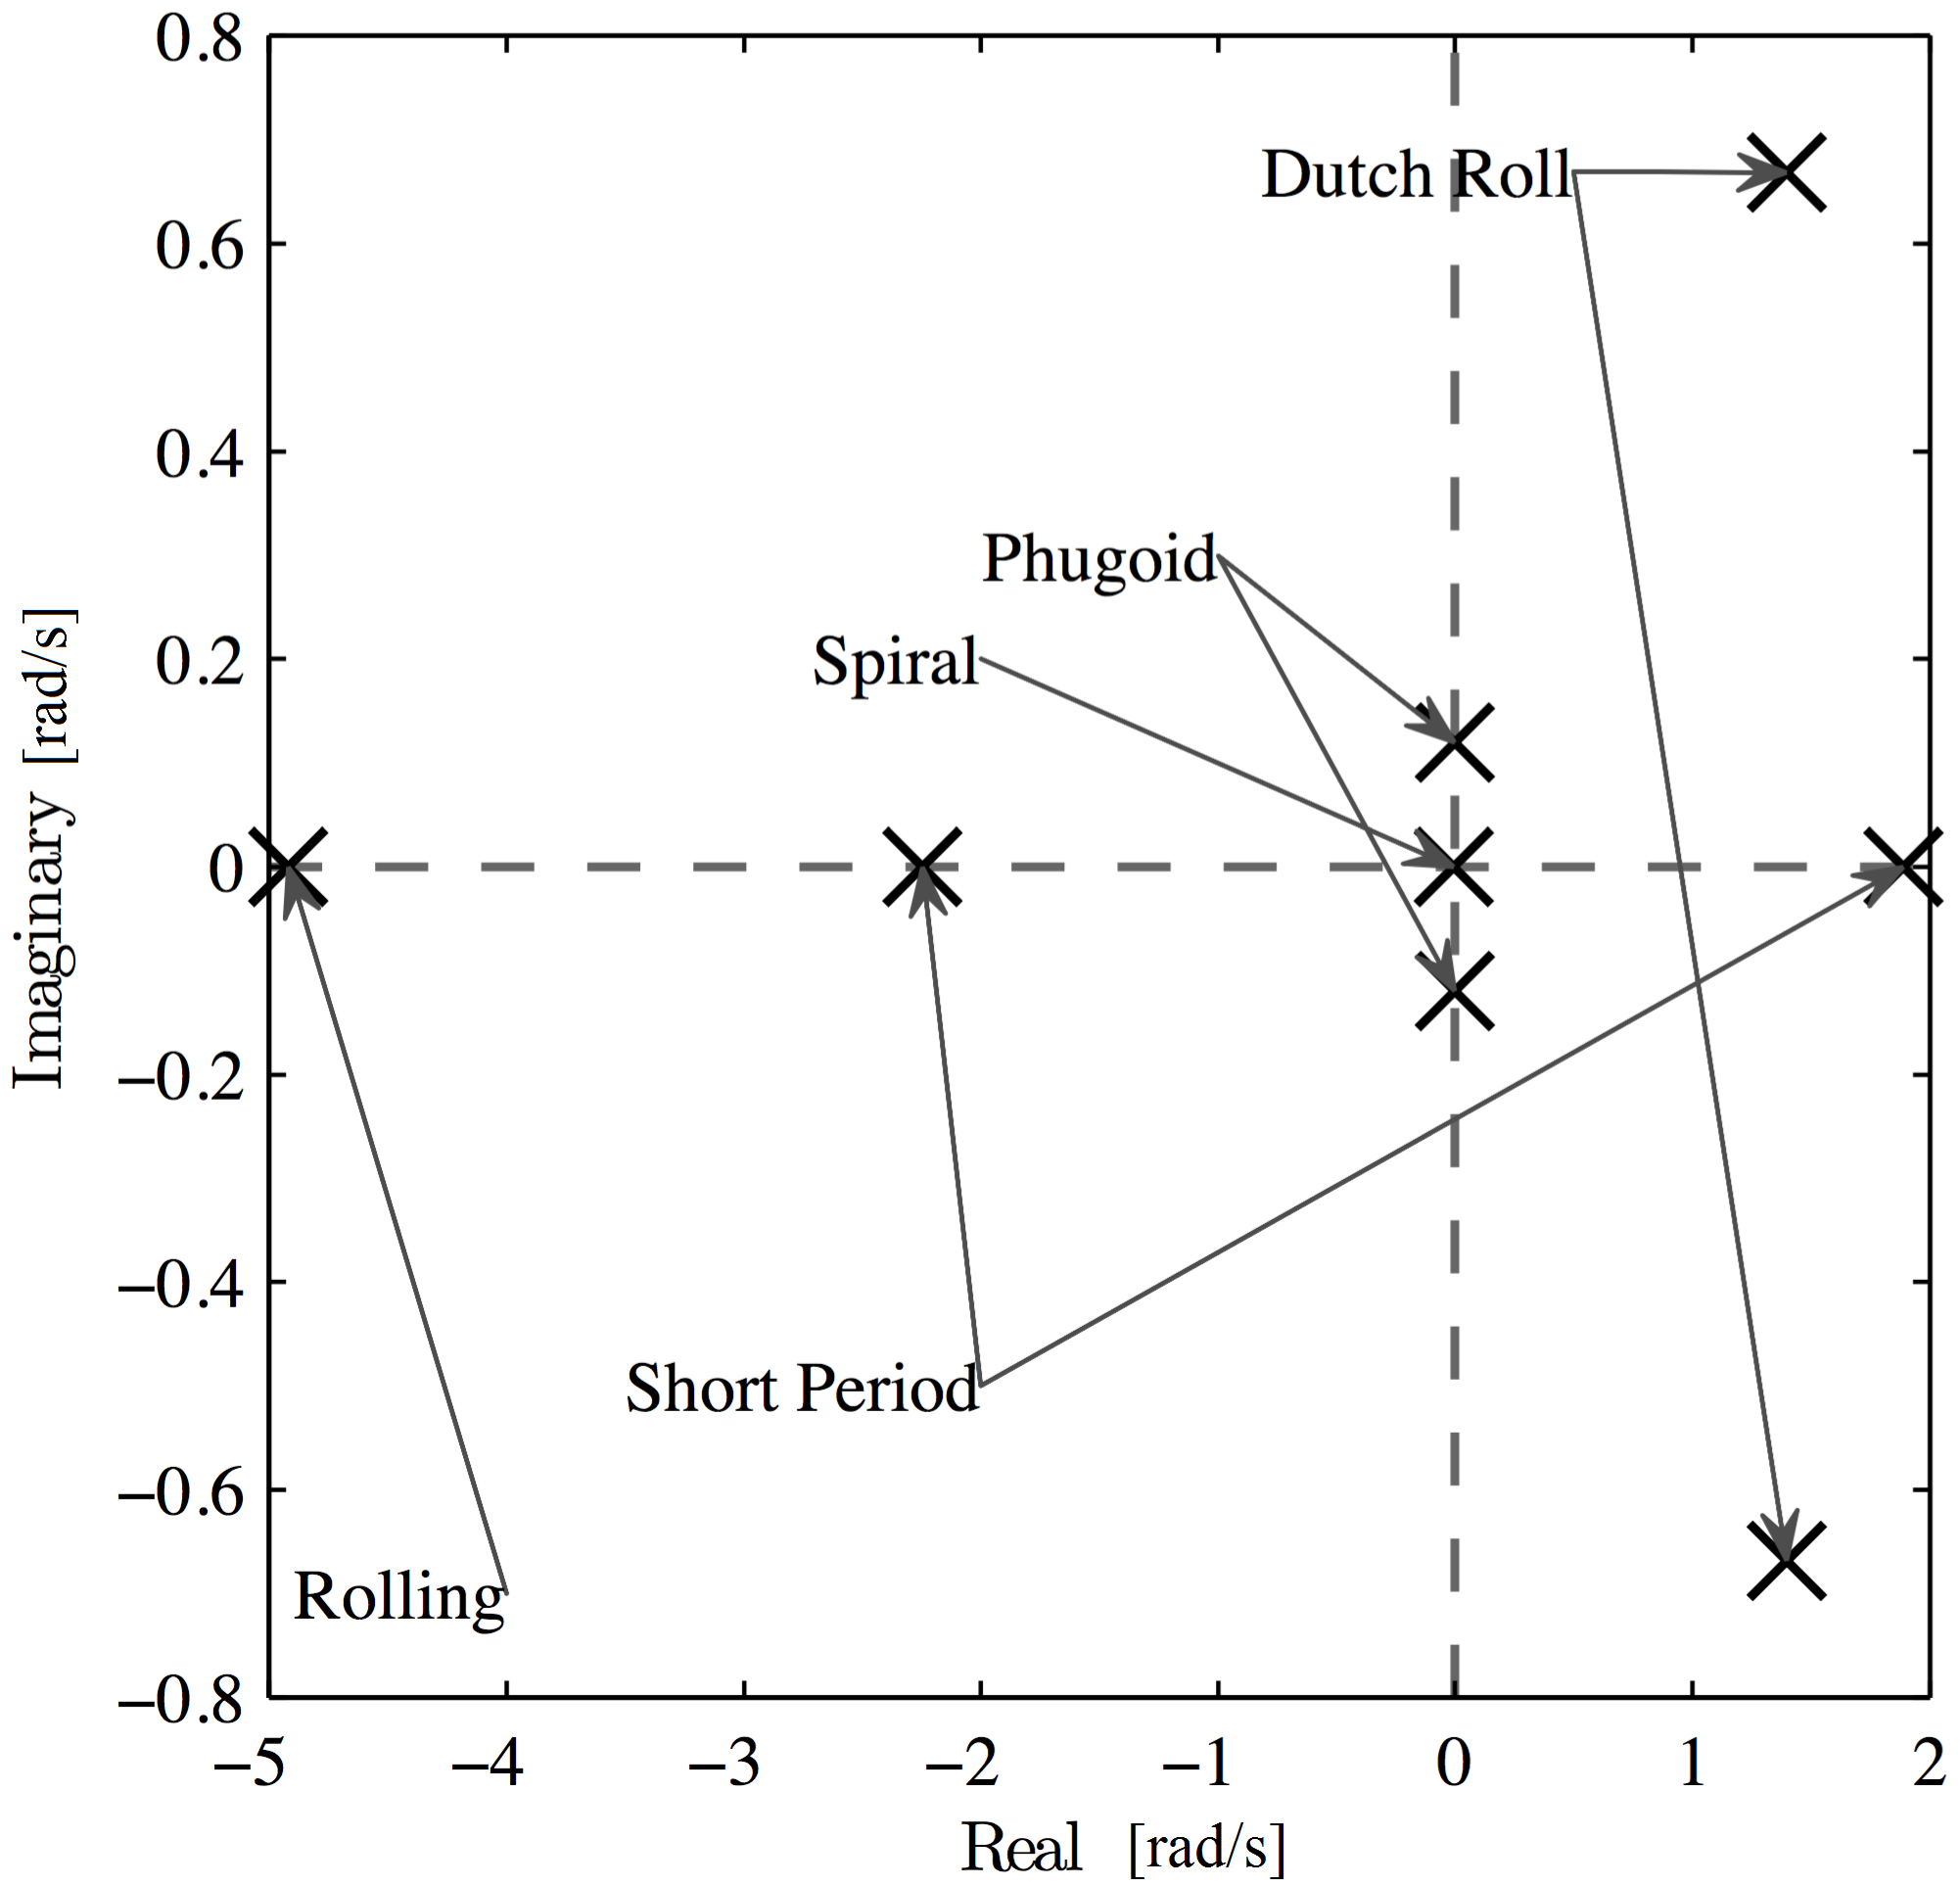
\includegraphics[width=4.0in]{\figurepath/openLoopPoles.png}
  \caption{Open-loop poles of $A$ for $M=6$, $h=80,000$ ft steady, level cruise\label{fig:poleplot}}
\end{figure}

The sensitivity analysis performed above indicates the presence of six flight modes.
These modes are explained below.
\begin{itemize}\itemsep2pt
  \item{\textbf{Short Period} ($\lambda_{1,3}$) \textemdash{} an unstable mode dominated by $\alpha$ and $q$. Relatively fast, purely real poles, with $\lambda_{1,3}\approx\pm2$.}
  \item{\textbf{Rolling} ($\lambda_{2}$) \textemdash{} a stable mode, dominated by $\beta$ and $p$. Fast, real pole at $\lambda_{2}=-4.9$.}
  \item{\textbf{Dutch-Roll} ($\lambda_{4,5}$) \textemdash{} an unstable mode, which is a combination of a rolling, pitching, and yawing motion in flight.}
  \item{\textbf{Phugoid} ($\lambda_{6,7}$) \textemdash{} a neutrally stable phugoid-type mode.}
  \item{\textbf{Velocity} ($\lambda_{8}$) \textemdash{} neutrally stable.}
  \item{\textbf{Spiral} ($\lambda_{9}$) \textemdash{} a slow, but stable mode.}
\end{itemize}
The eigenvalues corresponding to the different modes are shown in the pole plot in Figure~\ref{fig:poleplot}.
The pole corresponding to the velocity mode is dropped, since it has no affect on any of the other longitudinal dynamics.
This stability analysis was repeated at several other flight conditions, and revealed the same basic modes, although the pole locations and stability of some of the modes differed from the flight condition shown here.

\section{Model for Control Design}

The above sections presented the nonlinear equations of motion which describe the dynamics of the GHV, linearized these equations, and then analyzed them to determine the validity of the linearization, and decouple the linear system into several reduced order systems: the velocity, longitudinal, and lateral-directional subsystems.
The modal analysis showed the decoupling of the velocity, longitudinal, and lateral modes, allowing each of these three subsystems to be considered independently.
This allows the control design of the GHV to be simplified, by having to design three lower order controllers, as opposed to a single higher order controller.
The velocity and longitudinal subsystems are both single input systems.
The throttle input $u_{\text{th}}$ controls only the velocity $V_{T}$, and the elevator input $u_{\text{elv}}$ controls the longitudinal states.
The lateral subsystem is multi input, with the aileron $u_{\text{ail}}$ and tail $u_{\text{rud}}$ as control inputs.
Before the control design for each of the three subsystems is presented, a few paragraphs are devoted to providing some additional background on the types of uncertainty that are present in the hypersonic vehicle and as in\ \eqref{eqn.wholeSystemUncertain}, and that are studied in the simulation results presented in this chapter.

\subsection{Model Uncertainty}

A model is only a mathematical representation of a system or process, and so the presence of uncertainty in any plant model is inevitable.
This is particularly true in the case of a hypersonic vehicles, due in part to engine/airframe coupling, complex shock interactions, flexible effects, and unsteady aerodynamics\ \cite{mcruer.hypersonic.1991,schmidt.dynamics.1992,rudd.hypersonic.2010}.
When building a more conventional vehicle such as a subsonic transport aircraft, much wind tunnel and flight test data is collected, and the aerodynamic coefficients describing the aircraft can in general be determined with a high level of accuracy\ \cite{maine.coefficients.1981,morelli.parameters.1997}.
This data is difficult to obtain for a hypersonic vehicle, where wind tunnel testing is more difficult to do.
Additionally an extremely limited amount of hypersonic flight test data has ever been recorded, especially for air-breathing hypersonic vehicles.
Existing analytical techniques often fail to accurately predict the stability derivatives for air-breathing vehicles due to hypersonic flow assumptions which are violated due to the presence of the engine\ \cite{rudd.integrated.2000}.
The use of CFD has become increasingly used to model the aerodynamics of hypersonic vehicles, but there is still much work to be done.
Because of these challenges, uncertainties in the values of the aerodynamic properties, such as in the stability derivatives of up to several hundred percent, are possible in a hypersonic vehicle.

Additionally, loss in control effectiveness can occur through damage sustained during flight, as depicted in Figure~\ref{fig:flapdamage}, degradation over time, as well as for similar reasons as above: the aerodynamic forces and moments generated by a control surface deflection are different from those forces and moments as predicted through modeling.

\begin{figure}[H]
  \begin{center}
    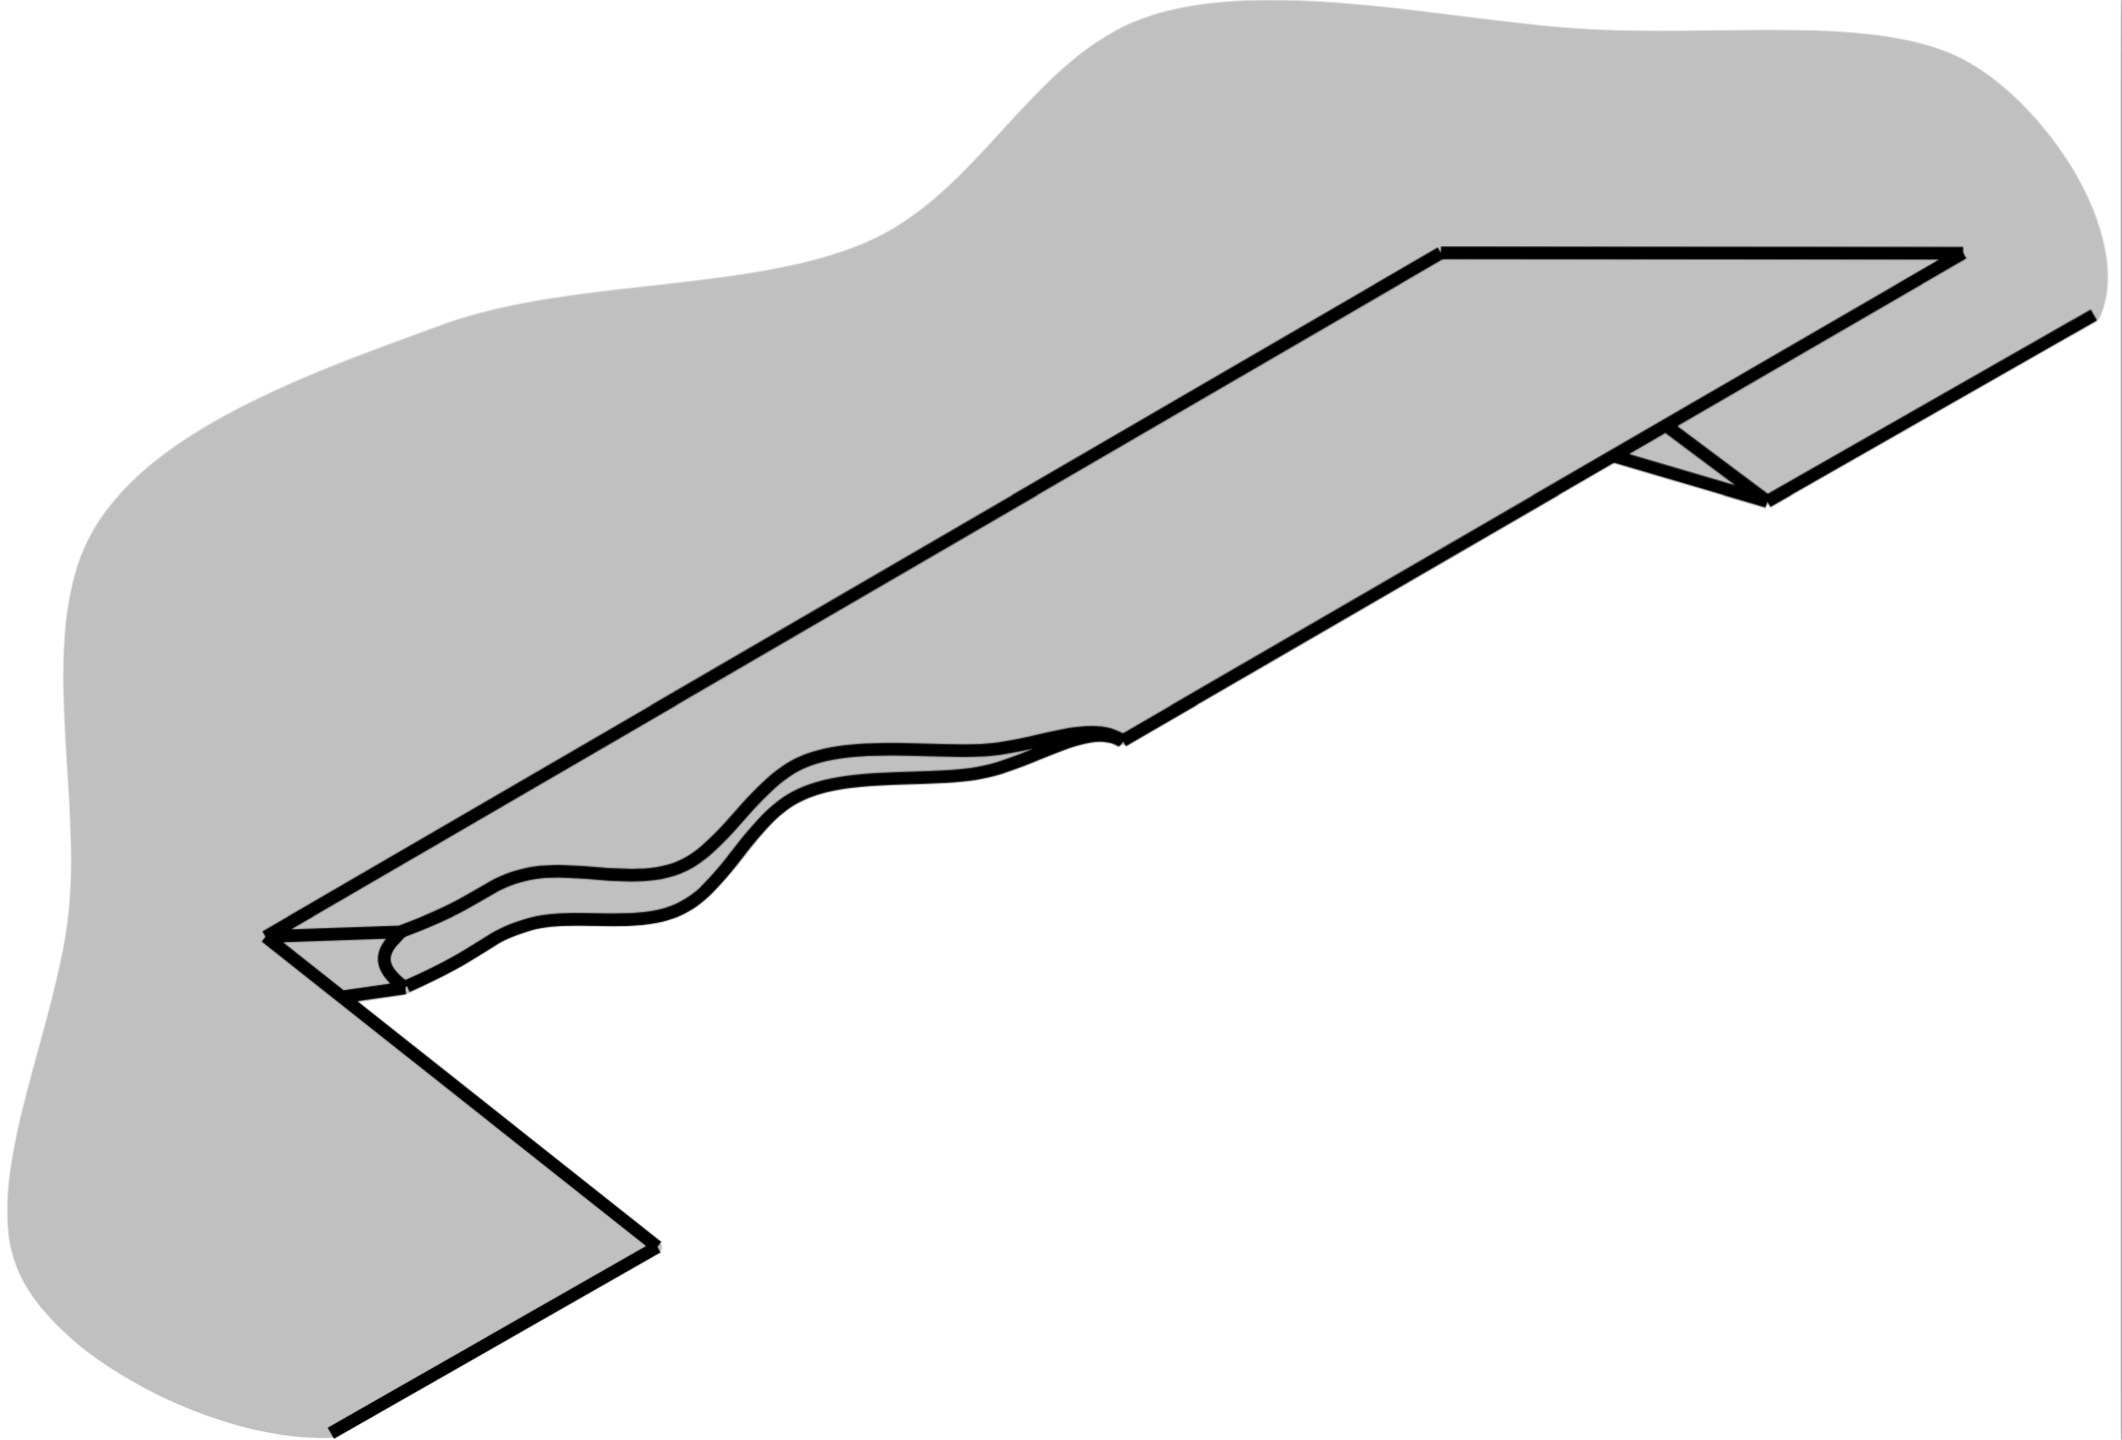
\includegraphics[width=2.0in]{\figurepath/flap2.png}
    \caption{Uncertainty in control effectiveness due to control surface damage\label{fig:flapdamage}}
  \end{center}
\end{figure}

Conventional aircraft can typically have significant variations in the center of gravity location.
These variations are minimized by careful loading of the aircraft, and by placing fuel tanks as close as is practicable to the center of gravity location so as to minimize the CG shift due to fuel burn.
The GHV will not be carrying any auxiliary payload, and it is the goal to have fuel tanks which are as close to the CG as possible.
Even so, uncertainty in the center of gravity location is inevitable and can greatly impact the stability of the vehicle.
Furthermore, changes in center-of-gravity location have a similar effect on the stability of the vehicle as shifts and uncertainty in the center-of-pressure location.
Thus, assuming uncertainty in center-of-gravity location also captures the effect of uncertainty in the center-of-pressure, which is very common in hypersonic vehicles.

\subsection{The Three Control Subsystems}

The three subsystems that the plant was separated into based on the distinct flight modes allowed for the design of multiple lower order controllers.
Each of the subsystems of the plant for which a controller will be designed is outlined here.

\subsubsection{Velocity Subsystem}

From the sensitivity analysis, the total velocity is decoupled from the rest of the states, allowing a separate controller to be designed to regulate and control only velocity.
The perturbation state, input, measured output, and regulated output used in the design of the velocity controller are given by
\begin{equation*}
  x_{p} = V_{T}
  \qquad
  u = \delta_{\text{th}}
  \qquad
  y_{p} = V_{T}
  \qquad
  z_{p} = V_{T}
\end{equation*}
For the velocity subsystem $n_{p}=1$ and $m=1$, and is a state-feedback problem.
Integral action is applied for tracking velocity reference commands.
That is $n_{ep}=1$.
The state-space matrices for the velocity subsystem represented by\ \eqref{eqn.xdotpunc} are given by
\begin{equation*}
  A_{p} = X_{v}
  \qquad
  B_{p} = X_{u_{\text{th}}}\cos(\alpha_{\text{eq}})
  \qquad
  C_{p} = 1
  \qquad
  C_{pz} = 1
  \qquad
  D_{pz} = 0
\end{equation*}

\subsubsection{Longitudinal Subsystem}

The uncertain, linear, longitudinal dynamics of the GHV in the form of\eqref{eqn.wholeSystemUncertain} are described as follows\ \cite{stengel.flightdynamics.2004}.
\begin{equation*}
  \begin{bmatrix}
    \dot{\alpha} \\
    \dot{q} \\
    \dot{\theta} \\
    \dot{h}
  \end{bmatrix}=
  \begin{bmatrix}
    \frac{Z_{\alpha}}{v_{\text{eq}}-Z_{\dot{\alpha}}} & \frac{v_{\text{eq}}+Z_{q}}{v_{\text{eq}}-Z_{\dot{\alpha}}} & -\frac{g\sin{\gamma_{\text{eq}}}}{v_{\text{eq}}-Z_{\dot{\alpha}}} & 0 \\
    M_{\alpha}+\frac{M_{\dot{\alpha}}Z_{\alpha}}{v_{\text{eq}}-Z_{\dot{\alpha}}} & M_{q}+\frac{M_{\dot{\alpha}}(v_{\text{eq}}+Z_{q})}{v_{\text{eq}}-Z_{\dot{\alpha}}} & M_{\theta}-\frac{M_{\dot{\alpha}}g\sin(\gamma_{\text{eq}})}{v_{\text{eq}}-Z_{\dot{\alpha}}} & 0 \\
    0 & 1 & 0 & 0 \\
    -v_{\text{eq}}\cos(\gamma_{\text{eq}}) & 0 & v_{\text{eq}}\cos(\gamma_{\text{eq}}) & 0 \\
  \end{bmatrix}
  \begin{bmatrix}
    \alpha \\
    q \\
    \theta \\
    h
  \end{bmatrix}+
  \begin{bmatrix}
    \frac{Z_{u_{\text{elv}}}}{v_{\text{eq}}-Z_{\dot{\alpha}}} \\
    M_{u_{\text{elv}}}+\frac{M_{\dot{\alpha}}Z_{u_{\text{elv}}}}{v_{\text{eq}}-Z_{\dot{\alpha}}} \\
    0 \\
    0
  \end{bmatrix}
  u_{\text{elv}}
\end{equation*}

\paragraph{Inner-loop}
Partitioning the longitudinal dynamics gives the inner-loop short-period dynamics as described by\ \eqref{eqn.innerLoopDynamicsUncertain} with plant matrices given by
\begin{equation*}
  \begin{gathered}
    A_{p} =
    \begin{bmatrix}
      \frac{Z_{\alpha}}{v_{\text{eq}}-Z_{\dot{\alpha}}} & \frac{v_{\text{eq}}+Z_{q}}{v_{\text{eq}}-Z_{\dot{\alpha}}} \\
      M_{\alpha}+\frac{M_{\dot{\alpha}}Z_{\alpha}}{v_{\text{eq}}-Z_{\dot{\alpha}}} & M_{q}+\frac{M_{\dot{\alpha}}(v_{\text{eq}}+Z_{q})}{v_{\text{eq}}-Z_{\dot{\alpha}}} \\
    \end{bmatrix}
    \qquad
    B_{p} =
    \begin{bmatrix}
      \frac{Z_{u_{\text{elv}}}}{v_{\text{eq}}-Z_{\dot{\alpha}}} \\
      M_{u_{\text{elv}}}+\frac{M_{\dot{\alpha}}Z_{u_{\text{elv}}}}{v_{\text{eq}}-Z_{\dot{\alpha}}} \\
    \end{bmatrix} \\[8pt]
    B_{gd} =
      \begin{bmatrix}
      -\frac{g\sin{\gamma_{\text{eq}}}}{v_{\text{eq}}-Z_{\dot{\alpha}}} & 0 \\
      M_{\theta}-\frac{M_{\dot{\alpha}}g\sin(\gamma_{\text{eq}})}{v_{\text{eq}}-Z_{\dot{\alpha}}} & 0 \\
    \end{bmatrix}
    \qquad
    C_{p} =
    \begin{bmatrix}
      0 \\
      1
    \end{bmatrix}^{\top}
    \qquad
    C_{pz} =
    \begin{bmatrix}
      0 \\
      1
    \end{bmatrix}^{\top}
  \end{gathered}
\end{equation*}
and with $D_{pz} = 0$.
To design the inner-loop controller for the longitudinal subsystem, the $B_{gd}$ term in\ \eqref{eqn.innerLoopDynamicsUncertain} for the inner-loop short-period dynamics is neglected, giving a system in the form of\ \eqref{eqn.xdotpunc} where the state, control, measured output, and regulated output for the inner-loop linear longitudinal subsystem are given by
\begin{equation*}
  x_{p} =
  \begin{bmatrix}
    \alpha & q
  \end{bmatrix}^{\top}
  \hspace{0.5in}
  u = \delta_{e}
  \hspace{0.5in}
  y_{p} = q
  \hspace{0.5in}
  z_{p} = q
\end{equation*}
The pitch rate is measurable but the angle of attack is not.
The inner-loop control goal is to track pitch rate commands $z_{p,\text{cmd}}=q_{\text{cmd}}$.

\paragraph{Outer-loop}
The plant matrices for the outer-loop phugoid dynamics in the form of\ \eqref{eqn.outerLoopDynamics} are given by
\begin{equation*}
  \begin{gathered}
    A_{g} =
    \begin{bmatrix}
      0 & 0 \\
      v_{\text{eq}}\cos(\gamma_{\text{eq}}) & 0
    \end{bmatrix}
    \qquad
    B_{pg} =
    \begin{bmatrix}
      0 & 1 \\
      -v_{\text{eq}}\cos(\gamma_{\text{eq}}) & 0 \\
    \end{bmatrix}
    \qquad
    C_{g} =
    \begin{bmatrix}
      0 \\
      1
    \end{bmatrix}^{\top}
    \qquad
    C_{gz} =
    \begin{bmatrix}
      0 \\
      1
    \end{bmatrix}^{\top}
  \end{gathered}
\end{equation*}
with outer-loop state, measured output, and regulated output given by
\begin{equation*}
  x_{g} =
  \begin{bmatrix}
    \theta & h
  \end{bmatrix}^{\top}
  \hspace{0.5in}
  y_{g} = h
  \hspace{0.5in}
  z_{g} =h
\end{equation*}
The altitude is measurable but the pitch angle is not.

The inner-loop control design described in Ch.~\ref{ch.innerLoop} requires the state vector $x_{p}$ be augmented with the integral error state as in Eq.\ \eqref{eqn.xedot} resulting in a system of the form Eq.\ \eqref{eqn.uncsystem}.
The augmented state and output vector are
\begin{equation*}
  x=
  \begin{bmatrix}
    \alpha & q & x_{e}
  \end{bmatrix}^{\top}
  \hspace{0.5in}
  y=
  \begin{bmatrix}
    q & x_{e}
  \end{bmatrix}^{\top}
\end{equation*}

\subsubsection{Lateral-Directional Subsystem}

The uncertain, linear, lateral-directional dynamics of the GHV in the form of\eqref{eqn.wholeSystemUncertain} are described as follows\ \cite{stengel.flightdynamics.2004}.
\begin{equation}
  \label{eqn.lateralDirectionalDynamics}
  \begin{split}
    \begin{bmatrix}
      \dot{\beta} \\
      \dot{p} \\
      \dot{r} \\
      \dot{\phi} \\
      \dot{\psi} \\
    \end{bmatrix}
    =&
    \begin{bmatrix}
      \frac{Y_{\beta}}{V_{\text{eq}}} & \frac{Y_{p}}{V_{\text{eq}}} & \frac{Y_{r}-V_{\text{eq}}}{V_{\text{eq}}} & \frac{g\cos(\gamma_{\text{eq}})}{V_{\text{eq}}} & 0 \\
      L_{\beta} & L_{p} & L_{r} & L_{\phi} & 0 \\
      N_{\beta}+\frac{Y_{\beta}N_{\dot{\beta}}}{V_{\text{eq}}} & N_{p}+\frac{Y_{p}N_{\dot{\beta}}}{V_{\text{eq}}} & N_{r}+\frac{(Y_{r}-V_{\text{eq}})N_{\dot{\beta}}}{V_{\text{eq}}} & N_{\phi} & 0 \\
      0 & 1 & -\sin\gamma_{\text{eq}} & 0 & 0 \\
      0 & 0 & \cos\gamma_{\text{eq}} & 0 & 0 \\
    \end{bmatrix}
    \begin{bmatrix}
      \beta \\
      p \\
      r \\
      \phi \\
      \psi \\
    \end{bmatrix} \\
    &+
    \begin{bmatrix}
      \frac{Y_{u_{\text{ail}}}}{V_{\text{eq}}} & \frac{Y_{u_{\text{rud}}}}{V_{\text{eq}}} \\
      L_{u_{\text{ail}}} & L_{u_{\text{rud}}} \\
      N_{u_{\text{ail}}}+\frac{Y_{u_{\text{ail}}}B_{\dot{\beta}}}{V_{\text{eq}}} & N_{u_{\text{rud}}}+\frac{Y_{u_{\text{rud}}}B_{\dot{\beta}}}{V_{\text{eq}}} \\
      0 & 0 \\
      0 & 0 \\
    \end{bmatrix}
    \begin{bmatrix}
      u_{\text{ail}} \\
      u_{\text{rud}}
    \end{bmatrix}
  \end{split}
\end{equation}

\paragraph{Inner-loop}
Partitioning the lateral-directional dynamics gives the inner-loop dynamics as described by\ \eqref{eqn.innerLoopDynamicsUncertain} with plant matrices given by
\begin{equation*}
  \begin{gathered}
    A_{p}
    =
    \begin{bmatrix}
      \frac{Y_{\beta}}{V_{\text{eq}}} & \frac{Y_{p}}{V_{\text{eq}}} & \frac{Y_{r}-V_{\text{eq}}}{V_{\text{eq}}} & \\
      L_{\beta} & L_{p} & L_{r} \\
      N_{\beta}+\frac{Y_{\beta}N_{\dot{\beta}}}{V_{\text{eq}}} & N_{p}+\frac{Y_{p}N_{\dot{\beta}}}{V_{\text{eq}}} & N_{r}+\frac{(Y_{r}-V_{\text{eq}})N_{\dot{\beta}}}{V_{\text{eq}}} \\
    \end{bmatrix} \\[8pt]
    B_{p} =
    \begin{bmatrix}
      \frac{Y_{u_{\text{ail}}}}{V_{\text{eq}}} & \frac{Y_{u_{\text{rud}}}}{V_{\text{eq}}} \\
      L_{u_{\text{ail}}} & L_{u_{\text{rud}}} \\
      N_{u_{\text{ail}}}+\frac{Y_{u_{\text{ail}}}B_{\dot{\beta}}}{V_{\text{eq}}} & N_{u_{\text{rud}}}+\frac{Y_{u_{\text{rud}}}B_{\dot{\beta}}}{V_{\text{eq}}} \\
    \end{bmatrix}
    \qquad
    B_{gd} =
    \begin{bmatrix}
      \frac{g\cos(\gamma_{\text{eq}})}{V_{\text{eq}}} & 0 \\
      L_{\phi} & 0 \\
      N_{\phi} & 0 \\
    \end{bmatrix} \\[8pt]
    C_{p} =
    \begin{bmatrix}
      0 & 1 & 0 \\
      0 & 0 & 1 \\
    \end{bmatrix}
    \qquad
    C_{pz} =
    \begin{bmatrix}
      0 & 0 & 1
    \end{bmatrix}
    \qquad
    D_{pz} =
    \begin{bmatrix}
      0 & 0
    \end{bmatrix}
  \end{gathered}
\end{equation*}
To design the inner-loop controller for the lateral-directional subsystem, the $B_{gd}$ term in\ \eqref{eqn.innerLoopDynamicsUncertain} for the inner-loop dynamics is neglected, giving a system in the form of\ \eqref{eqn.xdotpunc} where the state, control, measured output, and regulated output for the inner-loop linear lateral-directional subsystem are given by
\begin{equation*}
  x_{p}=
  \begin{bmatrix}
    \beta & p & r
  \end{bmatrix}^{\top}
  \hspace{0.5in}
  u=
  \begin{bmatrix}
    \delta_{a} & \delta_{r}
  \end{bmatrix}^{\top}
  \hspace{0.5in}
  y_{p}=
  \begin{bmatrix}
    p & r & \phi
  \end{bmatrix}^{\top}
  \hspace{0.5in}
  z_{p} = r
\end{equation*}
The roll rate and yaw rate are measurable but the angle of sideslip is not.
The inner-loop control goal is to track roll rate commands $z_{p,\text{cmd}}=p_{\text{cmd}}$.

\paragraph{Outer-loop}

The plant matrices for the outer-loop dynamics in the form of\ \eqref{eqn.outerLoopDynamics} are given by
\begin{equation*}
  A_{g} =
  \begin{bmatrix}
    0 & 0 \\
    0 & 0 \\
  \end{bmatrix}
  \qquad
  B_{pg} =
  \begin{bmatrix}
    0 & 1 & -\sin\gamma_{\text{eq}} \\
    0 & 0 & \cos\gamma_{\text{eq}} \\
  \end{bmatrix}
\end{equation*}
with outer-loop state, measured output, and regulated output given by
\begin{equation*}
  x_{g} =
  \begin{bmatrix}
    \phi & \psi
  \end{bmatrix}^{\top}
  \qquad
  y_{g} = \psi
  \qquad
  z_{g} = \psi
\end{equation*}
Heading angle is measurable but the roll angle is not.

The inner-loop control design described in Ch.~\ref{ch.innerLoop} requires the state vector $x_{p}$ be augmented with the integral error state as in Eq.\ \eqref{eqn.xedot} resulting in a system of the form Eq.\ \eqref{eqn.uncsystem}.
The augmented state and output vector are
\begin{equation*}
  x=
  \begin{bmatrix}
    \beta & p & r & x_{e}
  \end{bmatrix}^{\top}
  \hspace{0.5in}
  y=
  \begin{bmatrix}
    p & r & x_{e}
  \end{bmatrix}^{\top}
\end{equation*}

\section{Simulation Implementation}

This section contains simulation results demonstrating and comparing the capabilities of the baseline and adaptive controllers when applied to the nonlinear evaluation model as depicted in Figure~\ref{fig.simblockdiagram}.
Before presenting the simulation studies showing the response of the vehicle to different commanded trajectories, some additional uncertainties which were used in the simulations are first outlined.

\begin{figure}[H]
  \begin{center}
    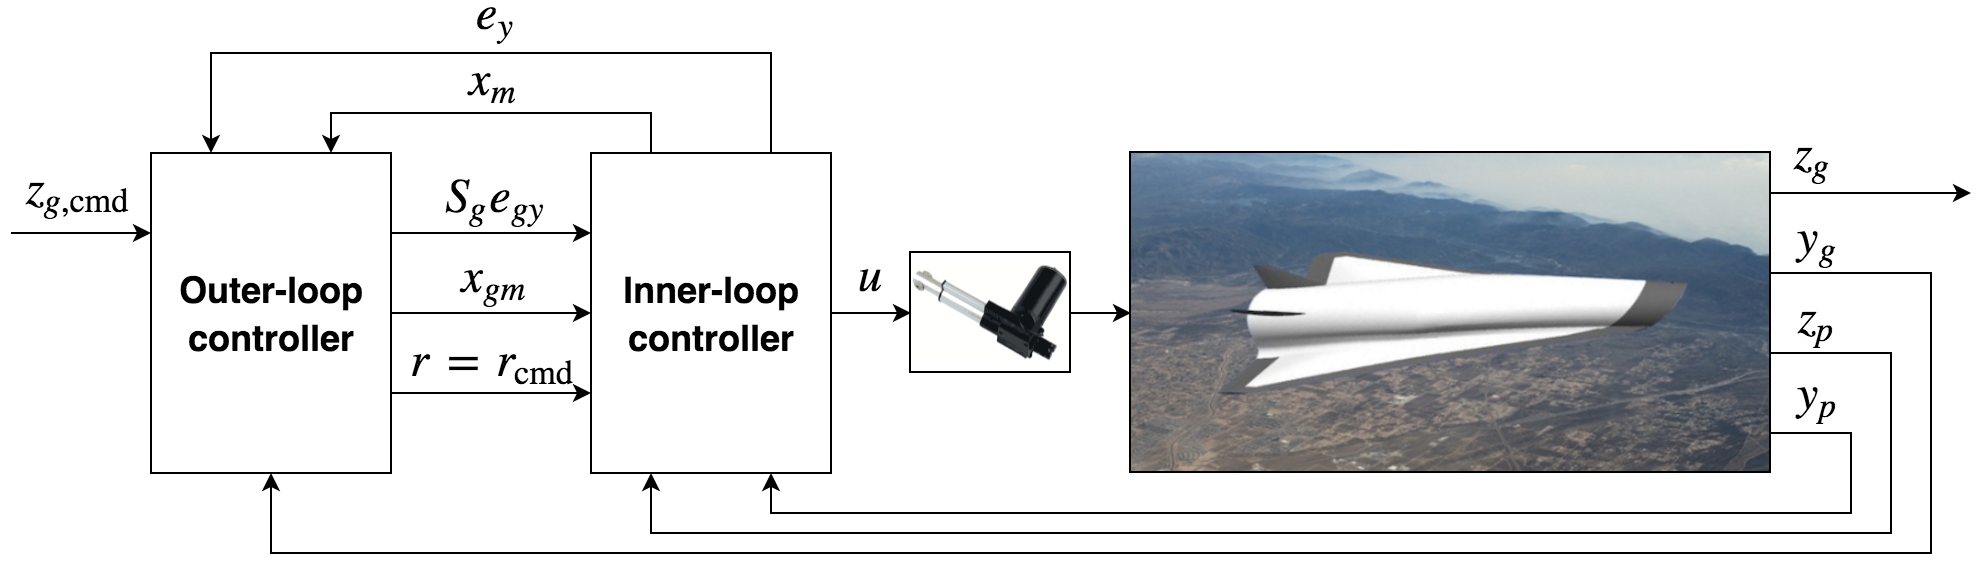
\includegraphics[width=6.5in]{\figurepath/simulationBlock.png}
    \vspace{-0.1in}
    \caption{Simulation block diagram.\label{fig.simblockdiagram}}
  \end{center}
\end{figure}

\subsection{Actuator Models}

\subsubsection{Throttle} The propulsion system is modeled as a first order system with a cutoff frequency of 10 rad/s, with transfer function
\begin{equation*}
  G_{\text{th}}(s)=\frac{\omega_{\text{th}}}{s+{\omega_{\text{th}}}}
\end{equation*}
While the physics of the engine happen on time scales order of magnitude faster than the rest of the dynamics, this simple model was proposed to capture fuel system delivery limits.

\subsubsection{Control Surfaces} Second order actuators with rate and deflection limits were included in the simulation model on all four of the aerodynamic control surfaces.
The transfer function for the control surface actuators is
\begin{equation*}
  G_{\text{cs}}(s)=\frac{{\omega_{n}}^{2}}{s^{2}+2\zeta\omega_{n}s+{\omega_{n}}^{2}}
\end{equation*}
and the block diagram for the control surfaces as implemented is shown in Figure~\ref{fig.actuatorBlock} where the signal $u_{\text{cmd}}$ is generated by the controller, and due to the actuator dynamics the actual control surface deflection is given by $u_{\text{sat}}$.
The relevant values used in the second order aerodynamic control surface actuator model are listed in Table~\ref{tab:actuator}.

\begin{figure}[H]
  \begin{center}
    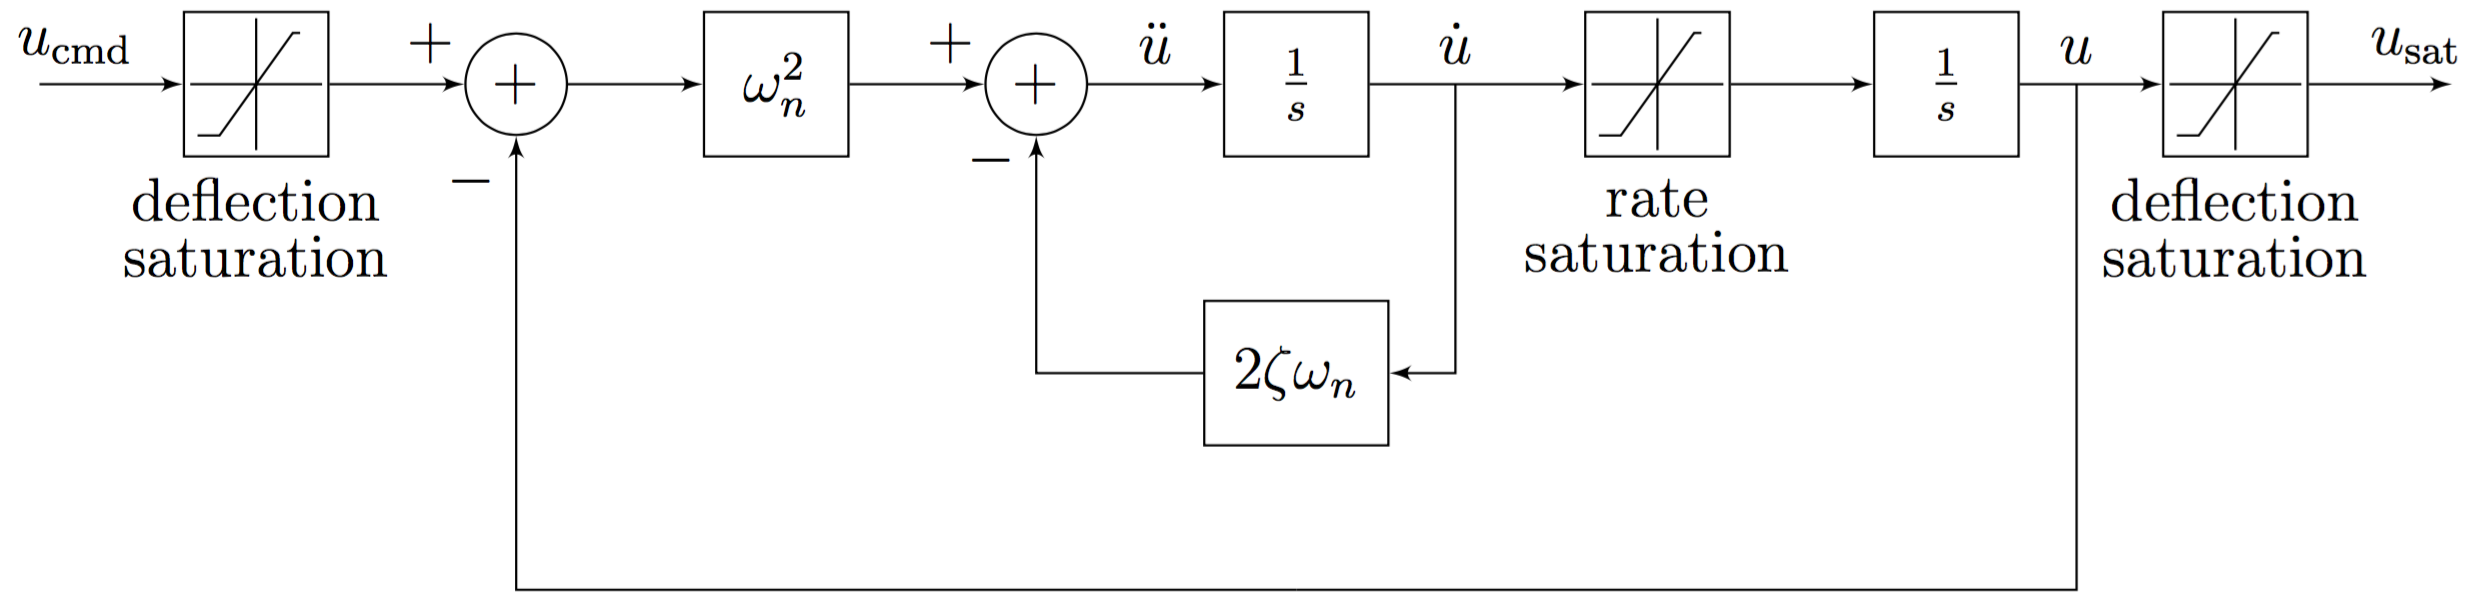
\includegraphics[width=5.5in]{\figurepath/actuatorBlock.png}
    \vspace{-0.1in}
    \caption{Second order actuator dynamics.\label{fig.actuatorBlock}}
  \end{center}
\end{figure}

\begin{table}[H]
  \centering
  \caption{Second order aerodynamic control surface actuator parameters\label{tab:actuator}}
  \begin{tabular}{llc}
    \toprule
    Parameter & Unit & Value \\ \midrule
    Surface deflection limit & [deg] & $-30$ to $30$ \\
    Surface rate limit & [deg/s] & $-100$ to $100$ \\
    Damping ratio $\zeta$ & & $0.7$ \\
    Natural frequency $\omega_{n}$ & [rad/s] & $150$ \\
    \bottomrule
  \end{tabular}
\end{table}

\begin{table}[H]
  \centering
  \caption{Components of trim state vector at nominal flight condition of Mach 5}
  \small
  \begin{tabular}{llr}
    \toprule
    State variable & Units & Value \\ \midrule
    $V_{T}$ & [ft/s] & 5866 \\
    $\alpha$ & [deg] & -0.59 \\
    $q$ & [deg/s] & 0 \\
    $\theta$ & [deg] & -0.59 \\
    $h$ & [ft] & 80,000 \\
    $\beta$ & [deg] & 0 \\
    $p$ & [deg/s] & 0 \\
    $r$ & [deg/s] & 0 \\
    $\phi$ & [deg] & 0 \\ \bottomrule
  \end{tabular}\label{tab:trimstate}
\end{table}

\section{Simulation Results}

The performance and robustness of the inner-loop adaptive controllers synthesized using the design model as represented by Eq.\ \eqref{eqn.xdotpunc} were evaluated by applying these controllers to an evaluation model\textemdash{}the hypersonic vehicle which is nonlinear and includes second order dynamics on the actuators which actuate the elevators, ailerons, and rudders, and the throttle response modeled as first order.
The numerical property values are listed in Table~\ref{tab:actuator}.
Uncertainties were introduced in the nonlinear model, which manifest themselves in the uncertain linear system as given in Eq.\ \eqref{eqn.xdotpunc}.
The uncertainty is as follows:
\begin{itemize}
  \item{Control effectiveness on all surfaces is reduced to 20\% of the nominal value.}
  \item{Center of gravity is shifted 0.7 feet rearward, effectively representing uncertainty in the center-of-pressure location.}
  \item{The rolling moment coefficient $C_{l}$ is reduced to 10\% of the nominal value.}
\end{itemize}

\subsection{Inner-Loop Response}\label{sec.numericalExample.innerLoop}

To evaluate the response of the inner-loop longitudinal controller, a 2 deg/s pitch rate doublet command was given.
The nominal response of the aircraft is shown in Figure~\ref{fig.baselineInnerNominalLongState} with the corresponding control inputs shown in~\ref{fig.baselineInnerNominalLongControl} for the case with no uncertainty and when using the baseline controller: $\Theta(t)=0$.
To evaluate the response of the lateral-directional controller, a 5 deg/s roll rate doublet command was given.
The nominal response of the aircraft is shown in Figure~\ref{fig.baselineInnerNominalLatrState} with the corresponding control inputs shown in Figure~\ref{fig.baselineInnerNominalLatrControl} for the case with no uncertainty and when using the baseline controller: $\Theta(t)=0$.

The purposed of both these inner-loop simulation responses is to show the nominal command tracking performance.
The introduction of uncertainty ultimately destabilizes the system when using the baseline controller, with the adaptive controller able to restore stability and ensure command tracking in the presence of these uncertainties.
However, to better examine the effect of these uncertainties on the vehicle performance when using both the baseline and adaptive controllers, this was done when using the outer-loop controller as well, as shown in the following section.

\newpage
\begin{figure}[H]
  \hspace{-0.5in}
  \noindent\makebox[7.5in]{%
  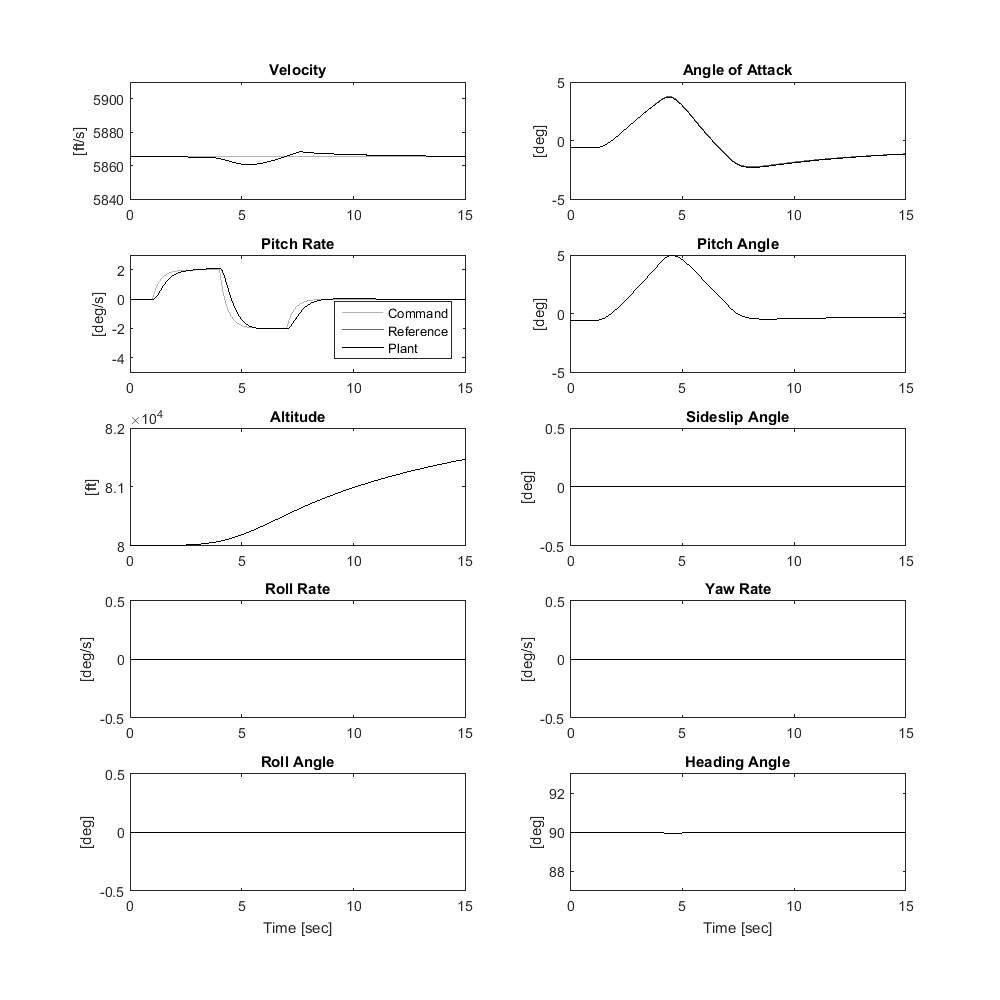
\includegraphics[width=7.5in]{\figurepath/baselineInnerNominalLongState.png}}
  \vspace{-1.0in}
  \caption{Plant states for baseline controller applied to nominal plant in response to a 2 degree per second pitch rate doublet.\label{fig.baselineInnerNominalLongState}}
\end{figure}

\newpage
\begin{figure}[H]
  \hspace{-0.5in}
  \noindent\makebox[7.5in]{%
  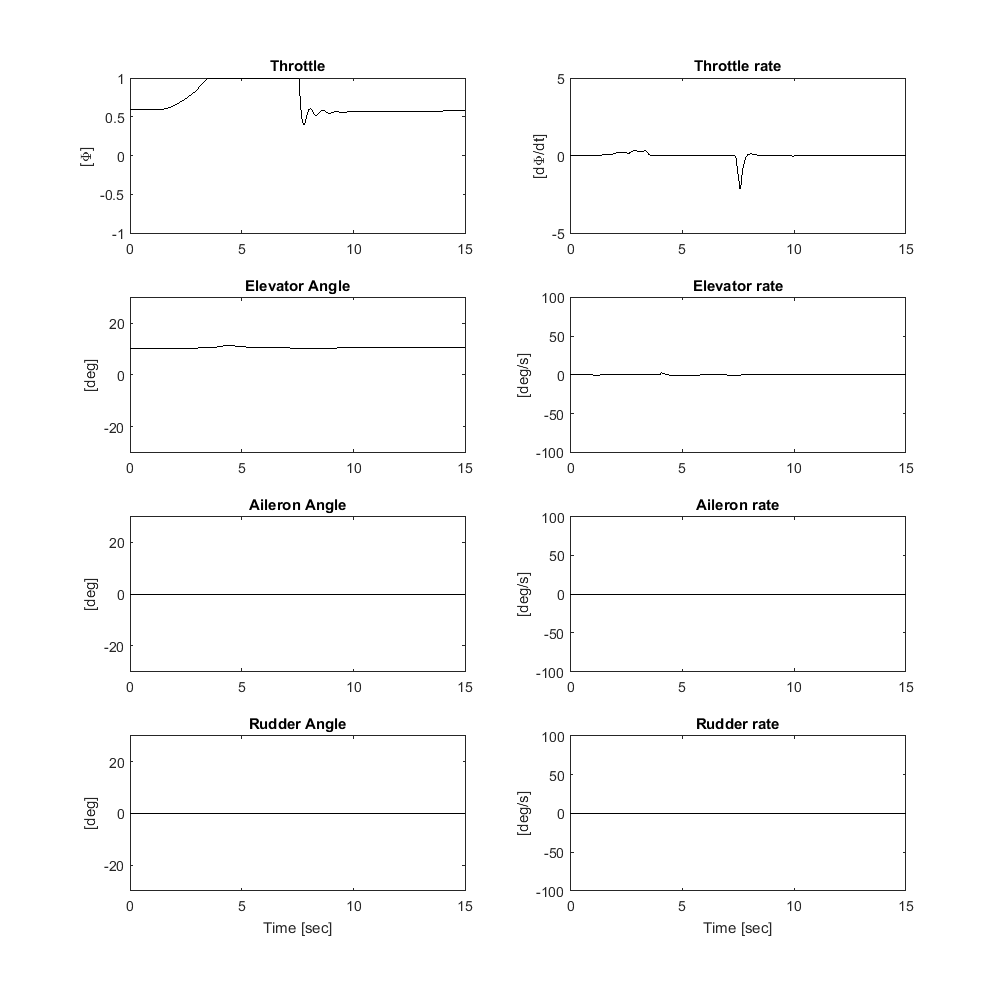
\includegraphics[width=7.5in]{\figurepath/baselineInnerNominalLongControl.png}}
  \vspace{-1.0in}
  \caption{Plant control input for baseline controller applied to nominal plant in response to a 2 degree per second pitch rate doublet.\label{fig.baselineInnerNominalLongControl}}
\end{figure}

\newpage
\begin{figure}[H]
  \hspace{-0.5in}
  \noindent\makebox[7.5in]{%
  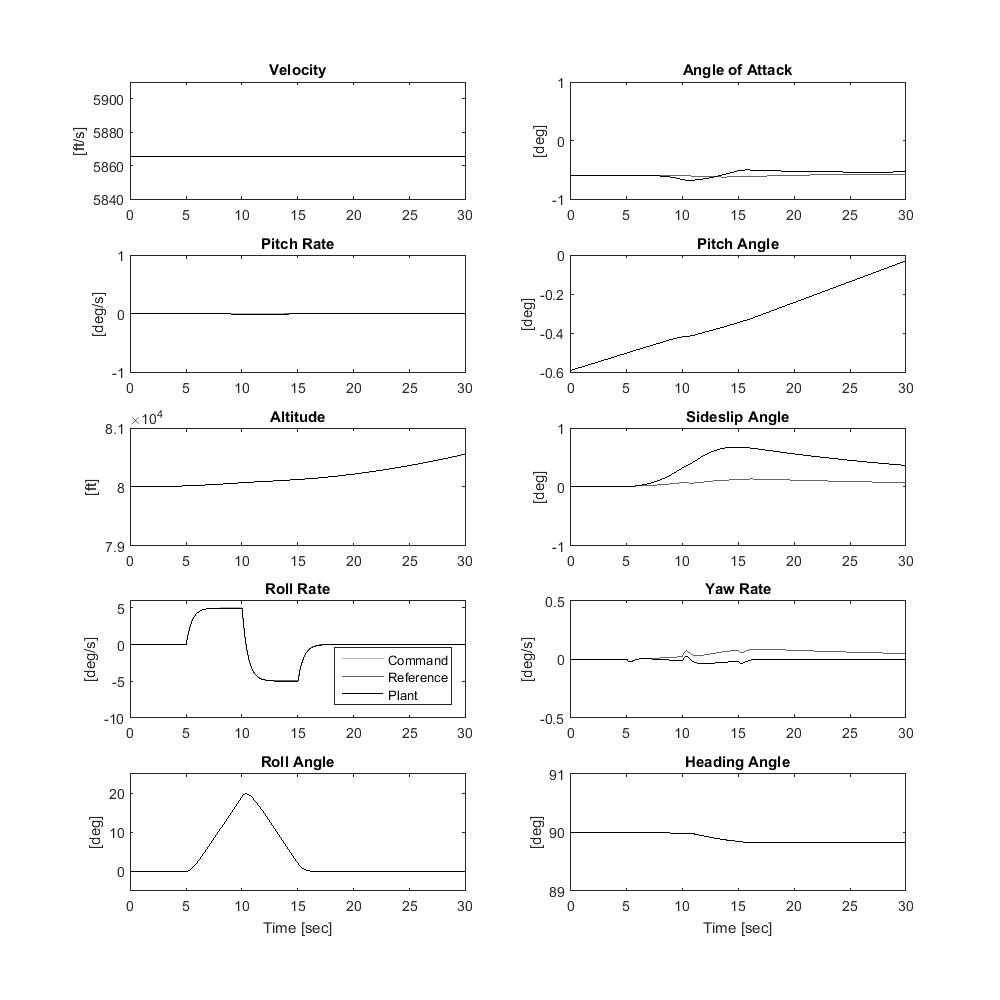
\includegraphics[width=7.5in]{\figurepath/baselineInnerNominalLatrState.png}}
  \vspace{-1.0in}
  \caption{Plant states for baseline controller applied to nominal plant in response to a 5 degree per second roll rate doublet.\label{fig.baselineInnerNominalLatrState}}
\end{figure}

\newpage
\begin{figure}[H]
  \hspace{-0.5in}
  \noindent\makebox[7.5in]{%
  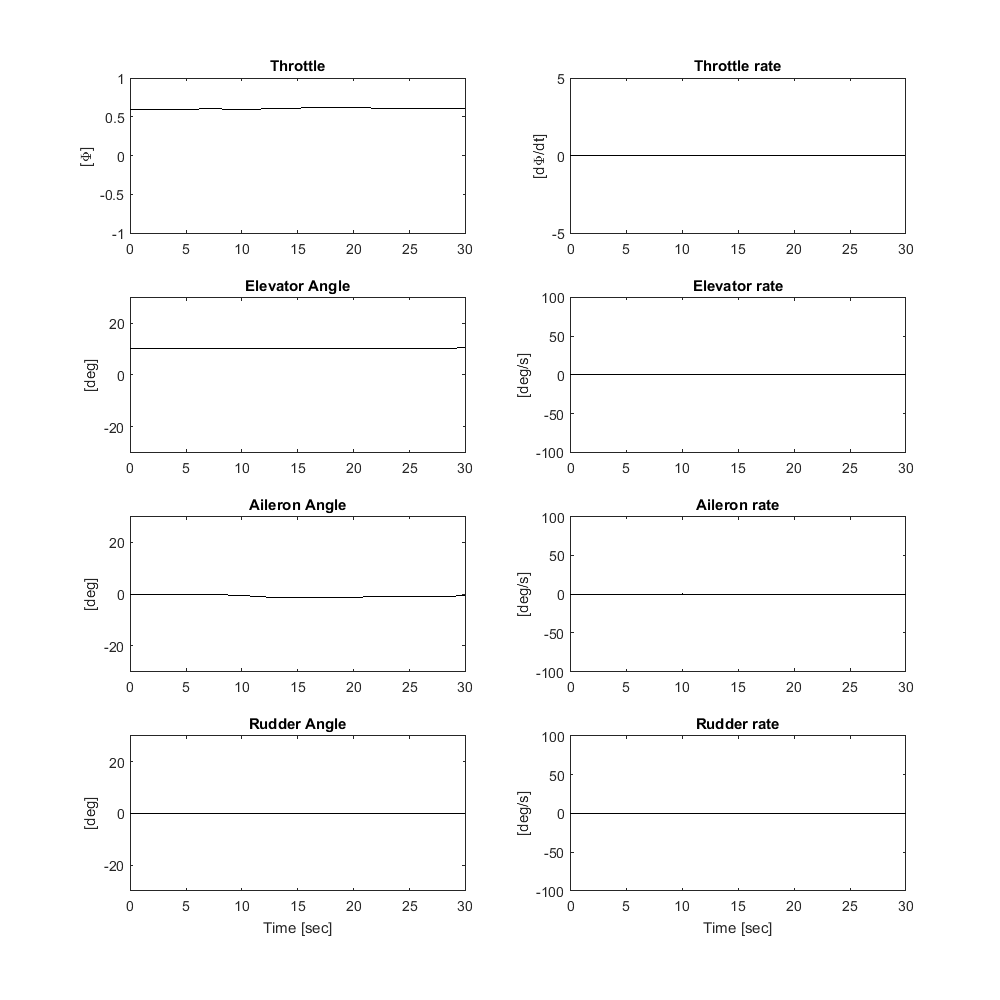
\includegraphics[width=7.5in]{\figurepath/baselineInnerNominalLatrControl.png}}
  \vspace{-1.0in}
  \caption{Plant control input for baseline controller applied to nominal plant in response to a 5 degree per second roll rate doublet.\label{fig.baselineInnerNominalLatrControl}}
\end{figure}


\subsection{Outer-Loop Response}\label{sec.numericalExample.outerLoop}

With the command tracking performance of the inner-loop controller verified in Sec.~\ref{sec.numericalExample.innerLoop}, the outer-loop was then designed around this inner-loop as described in Ch.~\ref{ch.outerLoop}.
The performance of the combined inner and outer-loop control structure was evaluated for both the longitudinal and lateral-directional control subsystems.

\subsubsection{Longitudinal Response}

To evaluate the longitudinal response of the GHV when using the closed-loop controllers, an altitude command to climb 1000 ft was given.
Figs.~\ref{fig.baselineNominalLongState} and~\ref{fig.baselineNominalLongControl} show the response in the nominal case, corresponding to the absence of uncertainty, and no adaptive control used.
That is $\Lambda=I$, $\Psi_{p}=0$, and $\Theta(t)=0$.
The response shows a smooth climb to the new altitude, while maintaining the desired heading, and without requiring large control magnitudes or rates.

Figs.~\ref{fig.baselineUncertainLongState} and~\ref{fig.baselineUncertainLongControl} show the response when the uncertainty was introduced, but with the adaptive controller still not used, that is $\Theta(t)=0$.
In this case, the uncertainty is sufficient to destabilize the GHV within a matter of seconds.

Figs.~\ref{fig.adaptiveUncertainLongState} and~\ref{fig.adaptiveUncertainLongControl} show the response when the adaptive controller is turned on. The result of this is closed-loop stability, and tracking of the altitude command.
However, during the course of adaptation some large undesirable oscillations are observed.

\subsubsection{Lateral-Directional Response}

To evaluate the lateral-direction response of the GHV when using the closed-loop controllers, a heading command of a right turn of 5 degrees was given.
Figs.~\ref{fig.baselineNominalLatrState} and~\ref{fig.baselineNominalLatrControl} show the response in the nominal case, corresponding to the absence of uncertainty, and no adaptive control used.
That is $\Lambda=I$, $\Psi_{p}=0$, and $\Theta(t)=0$.
The response shows a smooth turn to the new heading, while maintaining the desired altitude, and without requiring large control magnitudes or rates.

Figs.~\ref{fig.baselineUncertainLatrState} and~\ref{fig.baselineUncertainLatrControl} show the response when the uncertainty was introduced, but with the adaptive controller still not used, that is $\Theta(t)=0$.
In this case, the uncertainty is sufficient to destabilize the GHV within a matter of seconds.

Figs.~\ref{fig.adaptiveUncertainLatrState} and~\ref{fig.adaptiveUncertainLatrControl} show the response when the adaptive controller is turned on.
The result of this is closed-loop stability, and tracking of the heading command.
However, during the course of adaptation some large undesirable oscillations are observed.

\newpage
\begin{figure}[H]
  \hspace{-0.5in}
  \noindent\makebox[7.5in]{%
  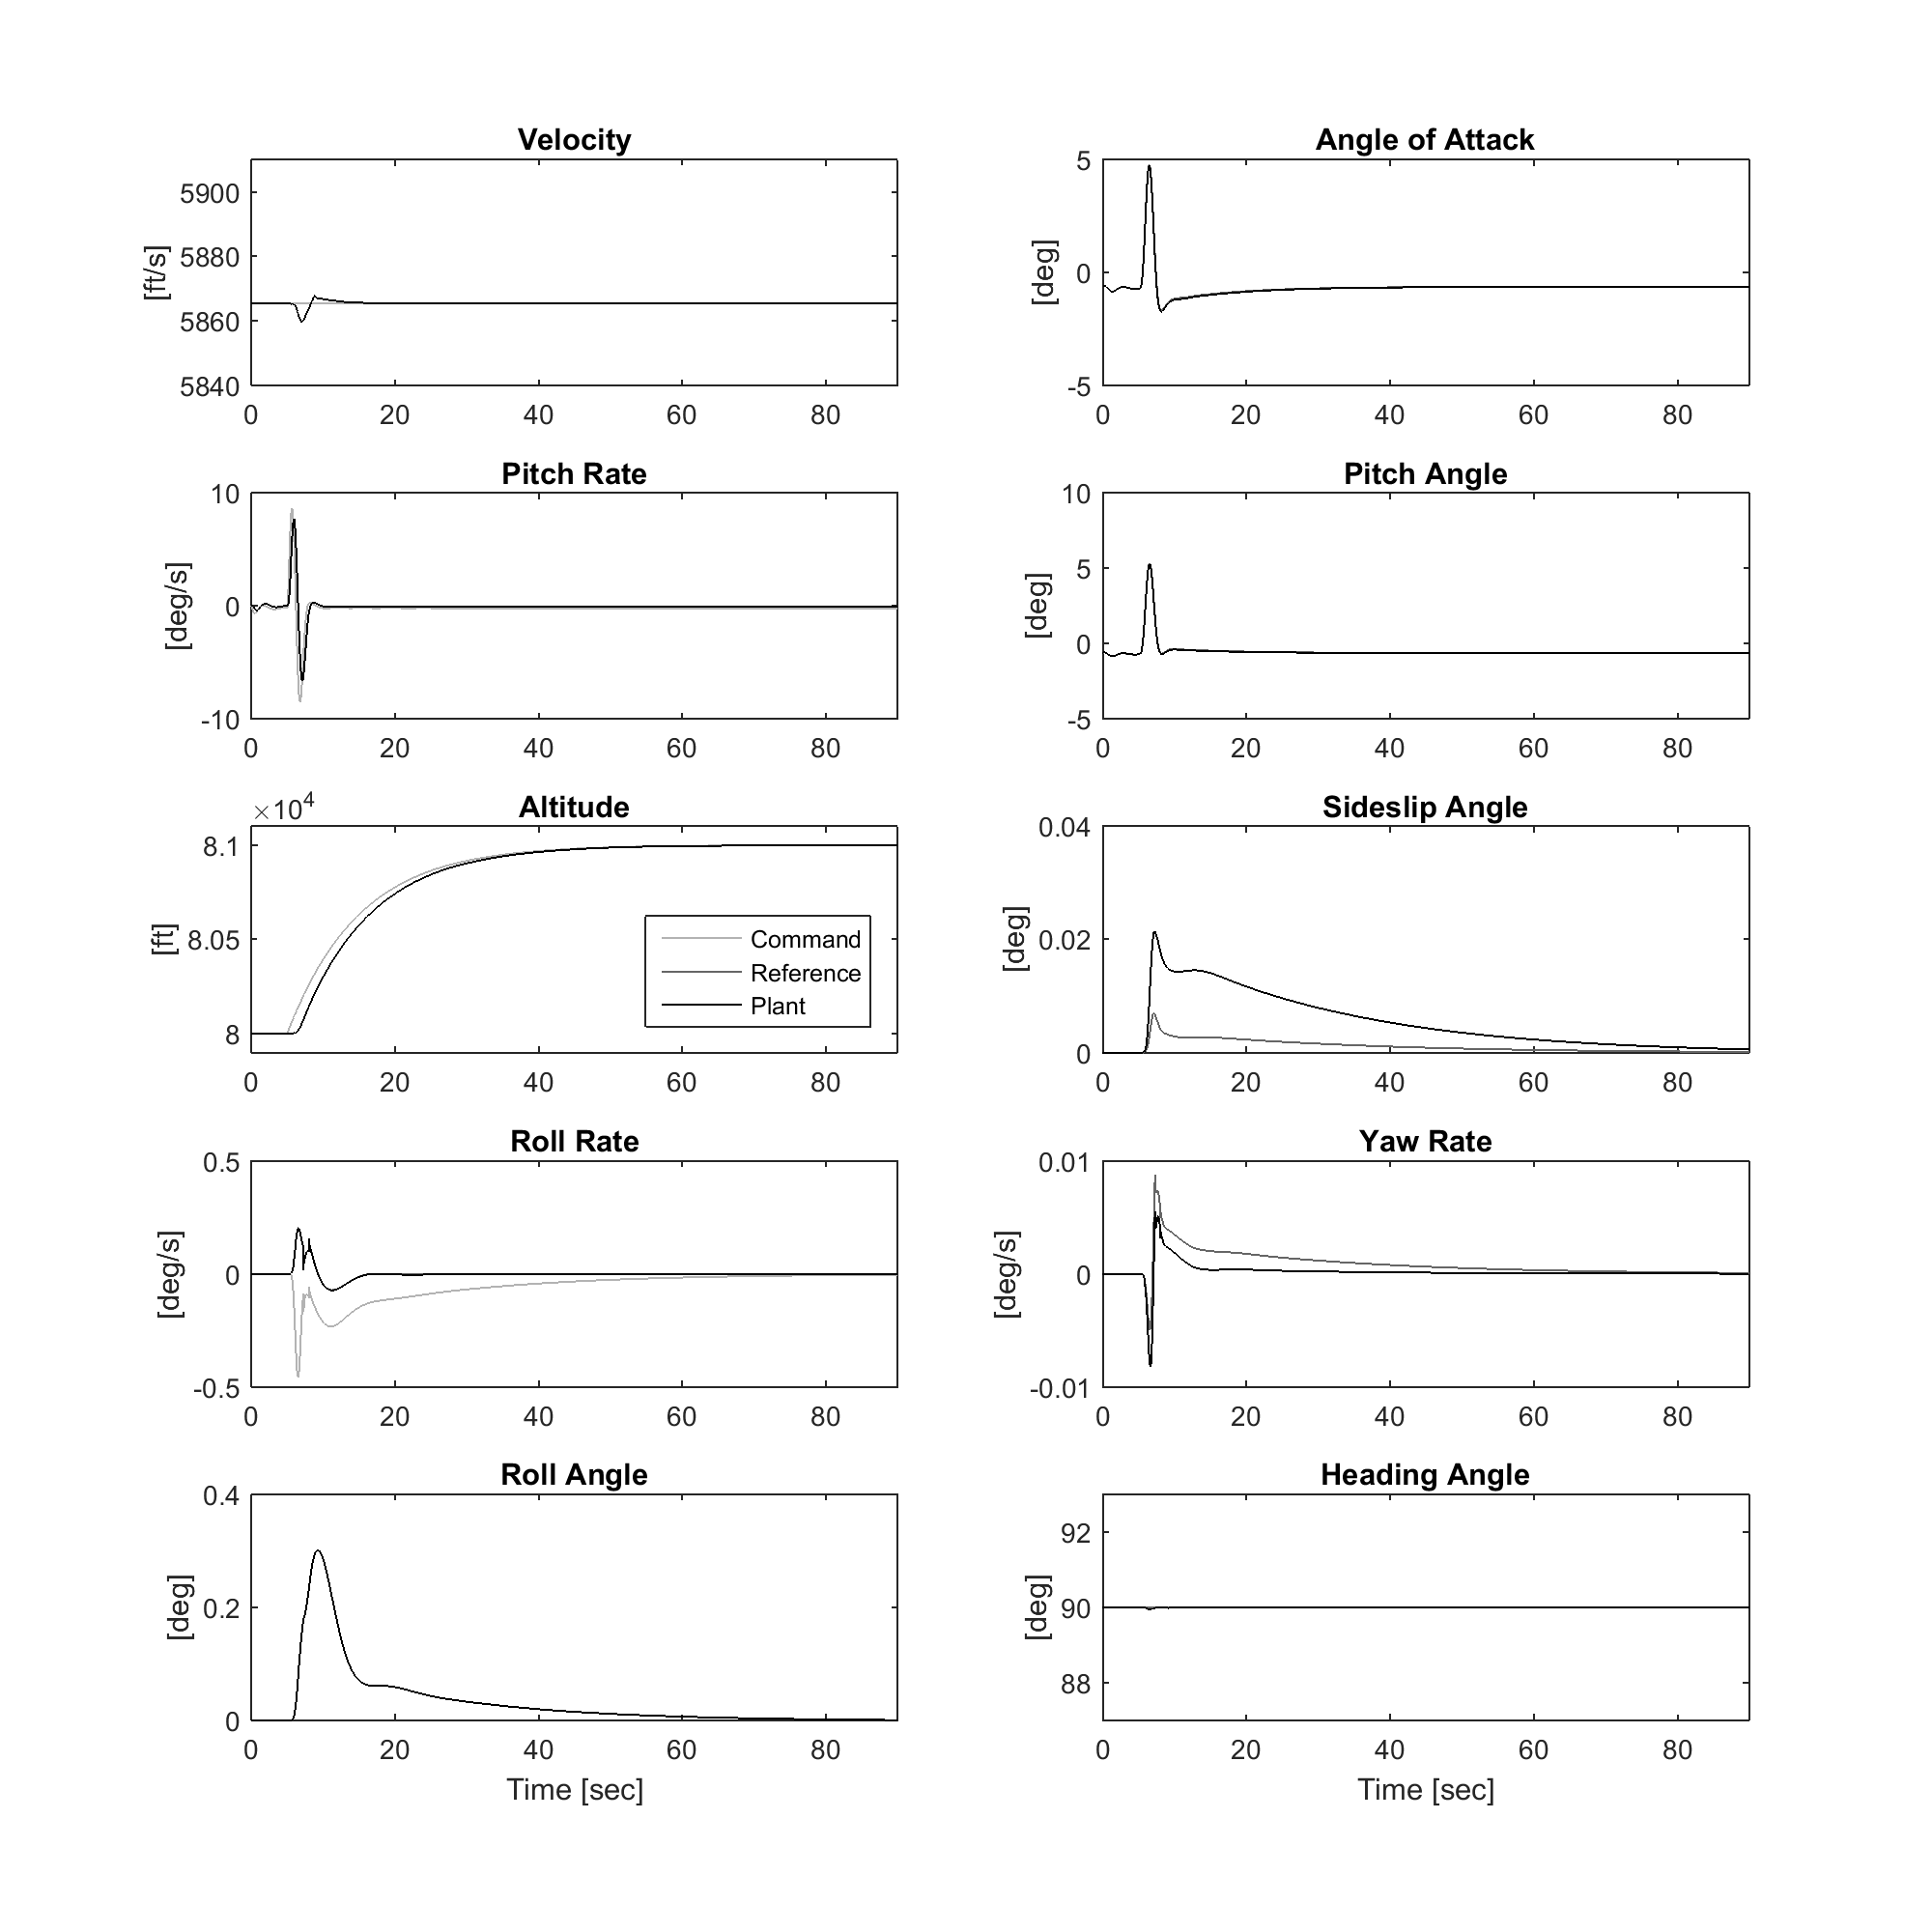
\includegraphics[width=7.5in]{\figurepath/baselineNominalLongState.png}}
  \vspace{-1.0in}
  \caption{Plant states for baseline controller applied to nominal plant in response to a 1000 ft.\ climb command.\label{fig.baselineNominalLongState}}
\end{figure}

\newpage
\begin{figure}[H]
  \hspace{-0.5in}
  \noindent\makebox[7.5in]{%
  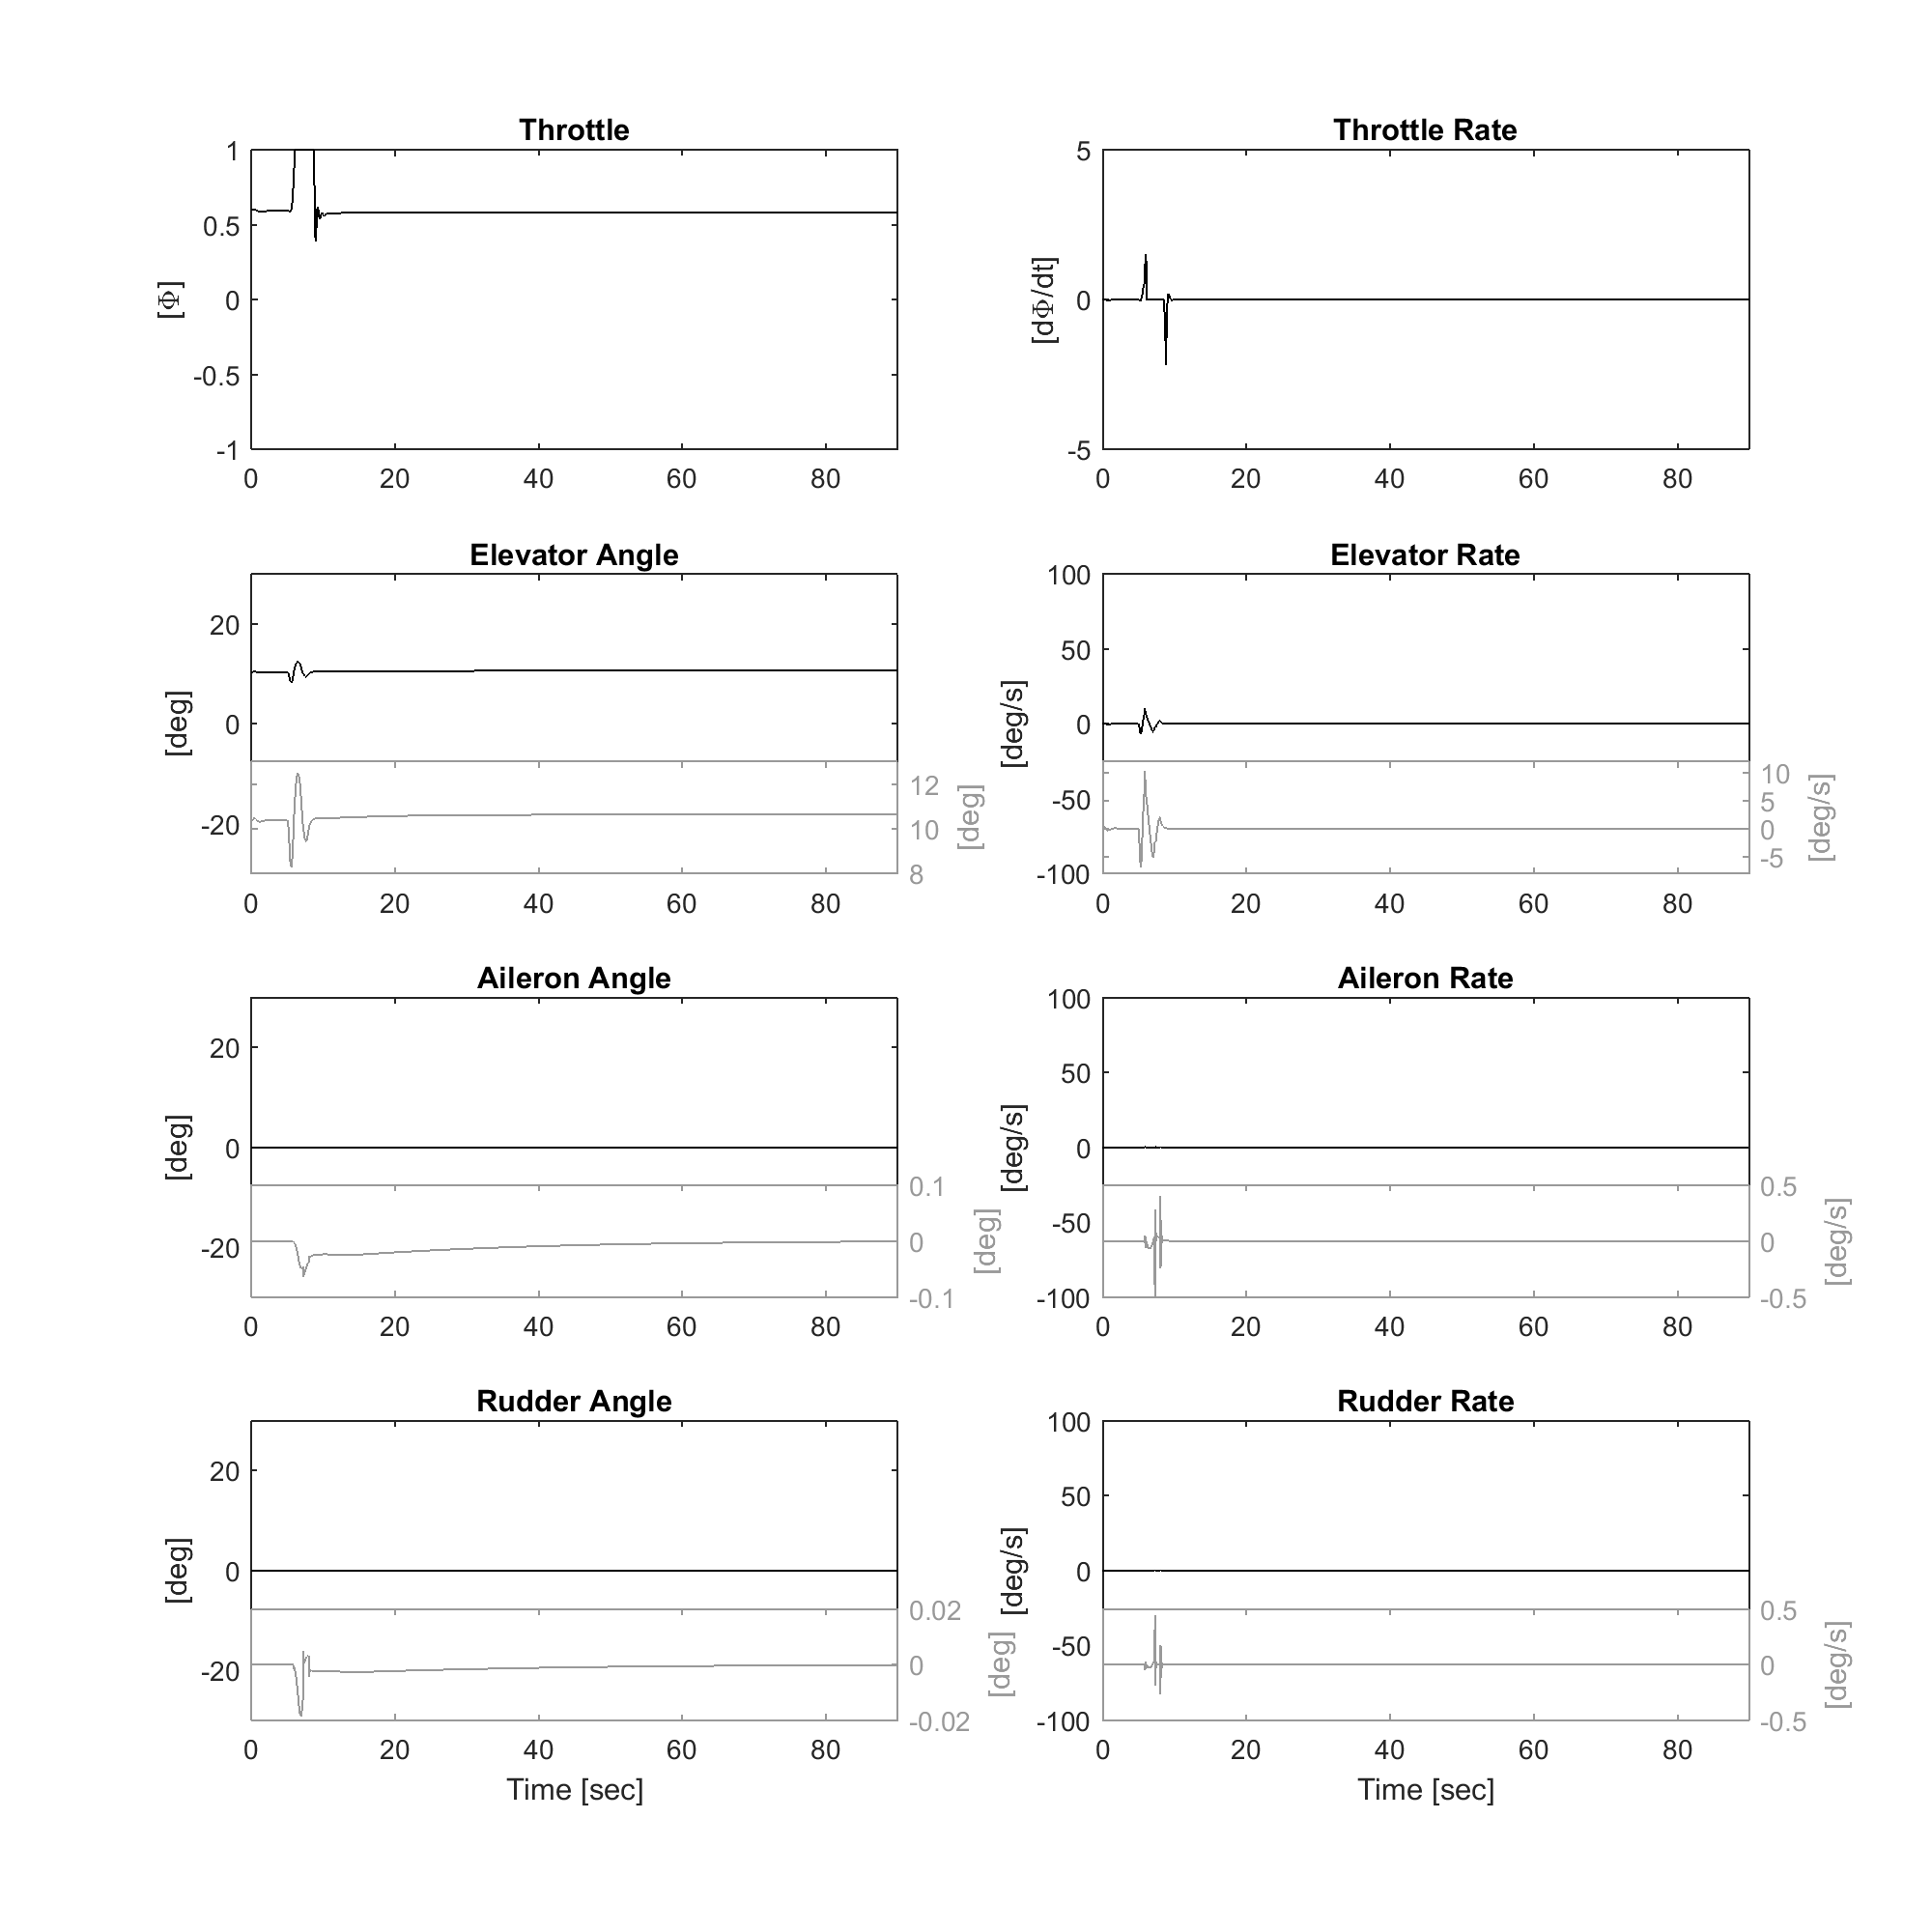
\includegraphics[width=7.5in]{\figurepath/baselineNominalLongControl.png}}
  \vspace{-1.0in}
  \caption{Plant control input for baseline controller applied to nominal plant in response to a 1000 ft.\ climb command.\label{fig.baselineNominalLongControl}}
\end{figure}

\newpage
\begin{figure}[H]
  \hspace{-0.5in}
  \noindent\makebox[7.5in]{%
  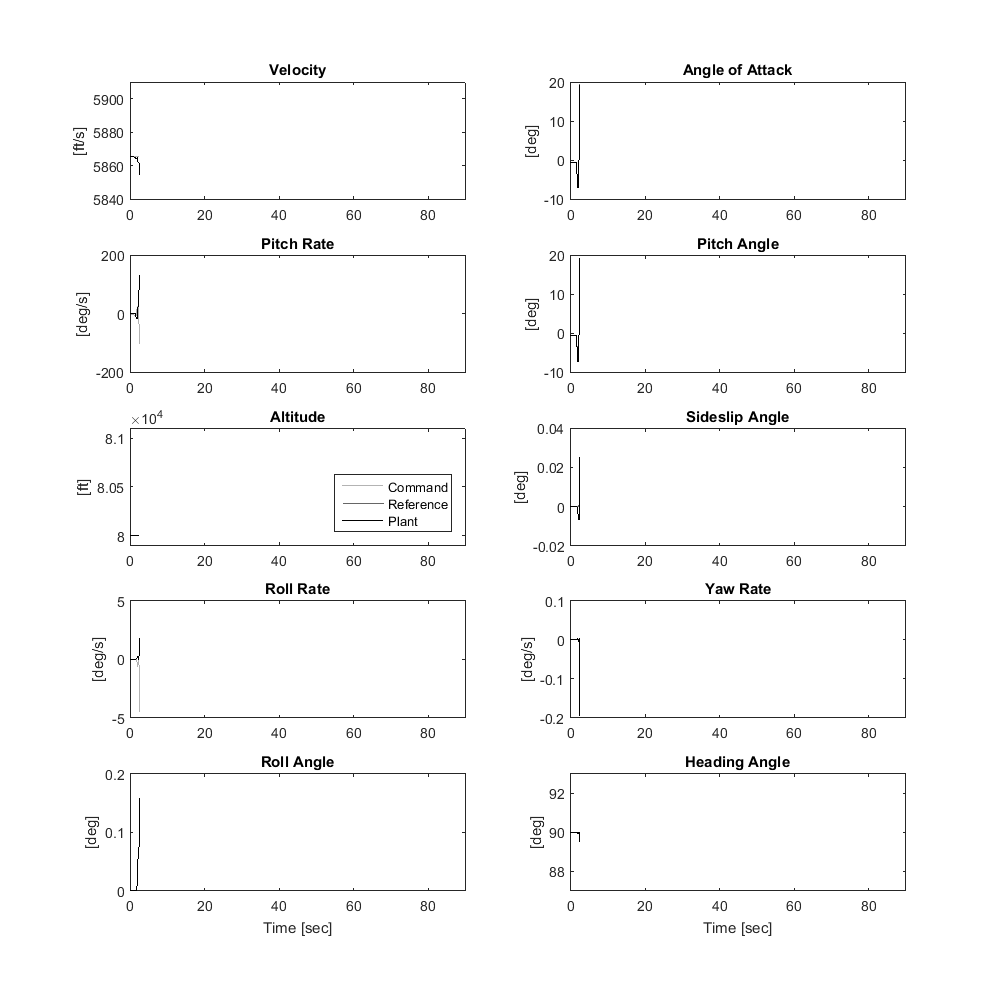
\includegraphics[width=7.5in]{\figurepath/baselineUncertainLongState.png}}
  \vspace{-1.0in}
  \caption{Plant states for baseline controller applied to uncertain plant in response to a 1000 ft.\ climb command.\label{fig.baselineUncertainLongState}}
\end{figure}

\newpage
\begin{figure}[H]
  \hspace{-0.5in}
  \noindent\makebox[7.5in]{%
  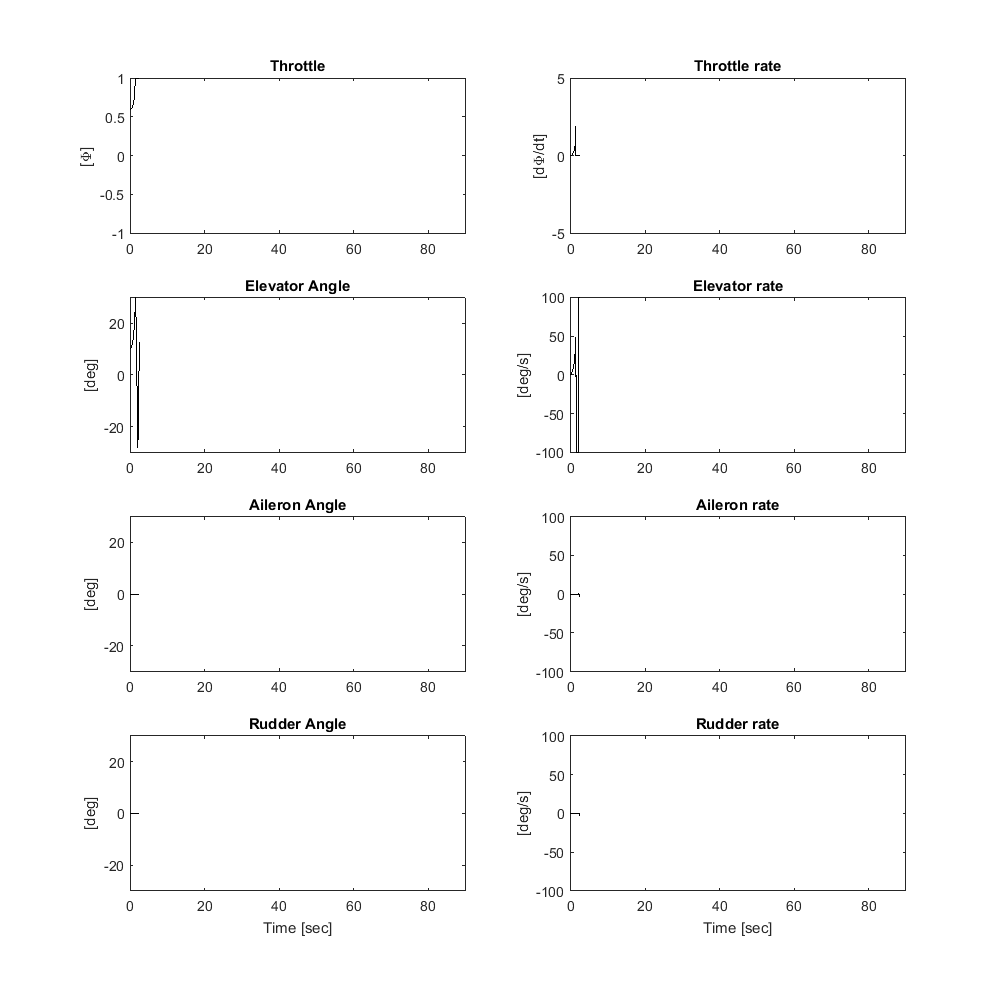
\includegraphics[width=7.5in]{\figurepath/baselineUncertainLongControl.png}}
  \vspace{-1.0in}
  \caption{Plant control input for baseline controller applied to uncertain plant in response to a 1000 ft.\ climb command.\label{fig.baselineUncertainLongControl}}
\end{figure}

\newpage
\begin{figure}[H]
  \hspace{-0.5in}
  \noindent\makebox[7.5in]{%
  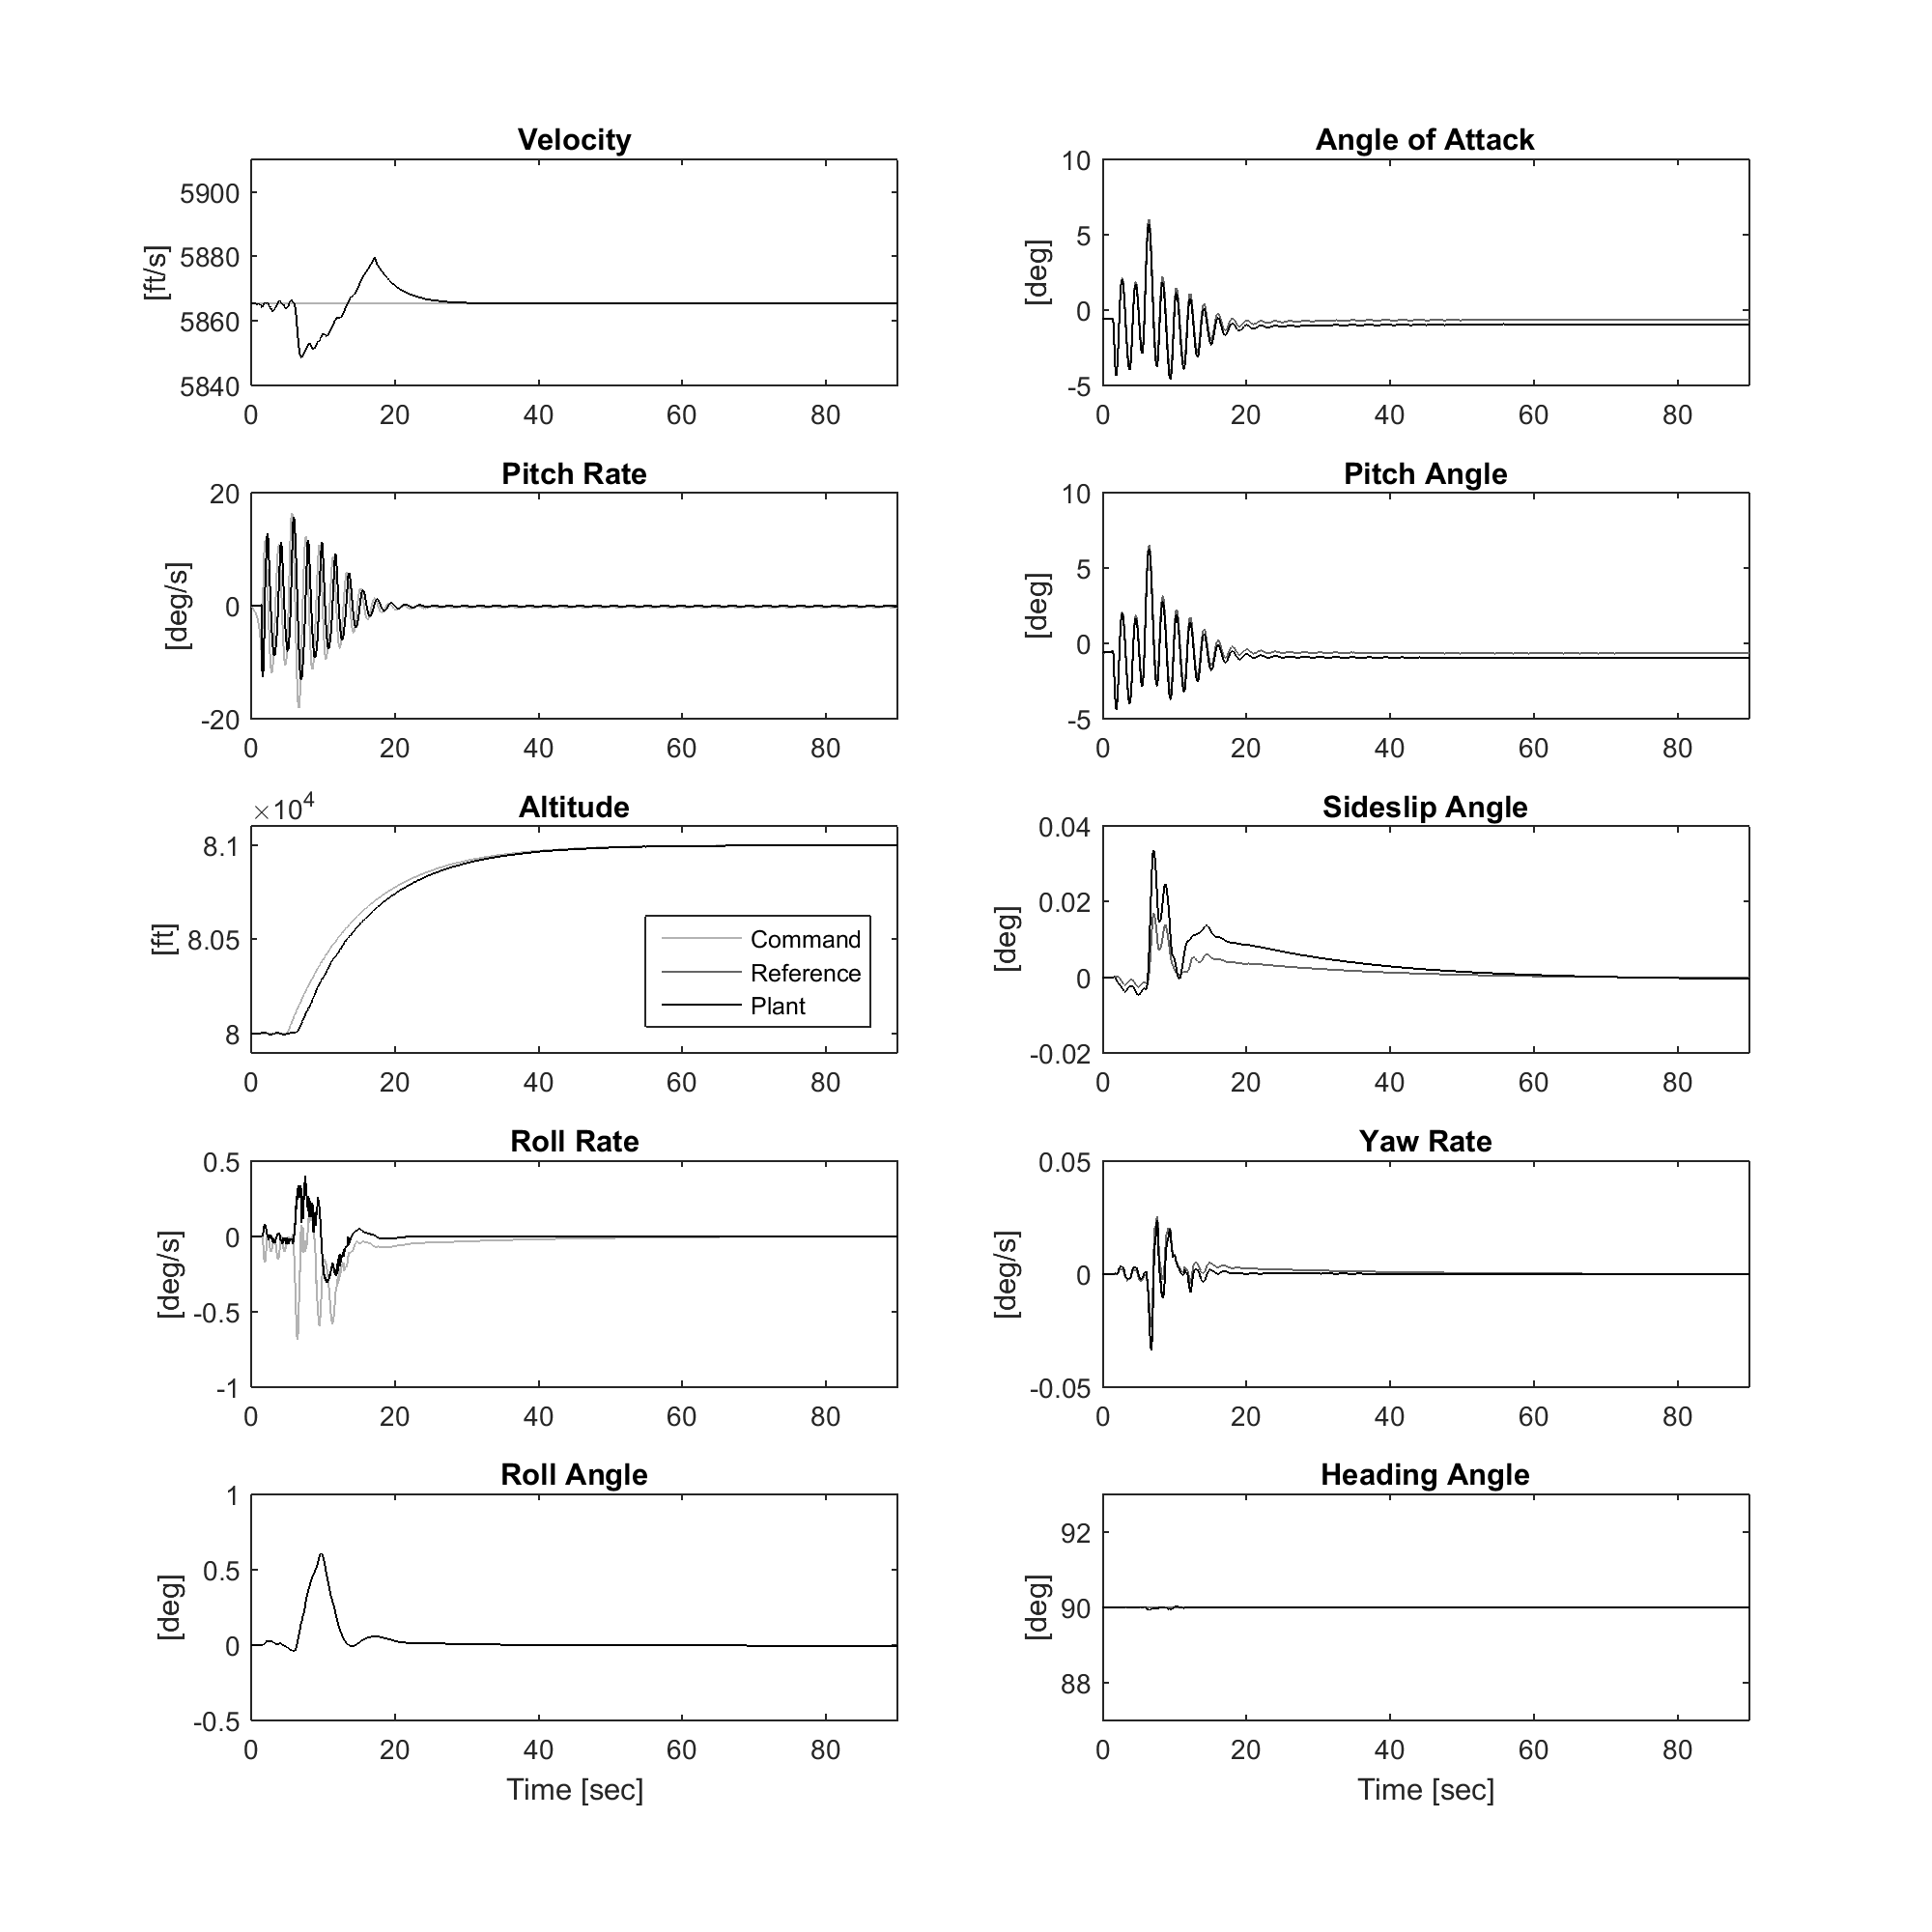
\includegraphics[width=7.5in]{\figurepath/adaptiveUncertainLongState.png}}
  \vspace{-1.0in}
  \caption{Plant states for adaptive controller applied to uncertain plant in response to a 1000 ft.\ climb command.\label{fig.adaptiveUncertainLongState}}
\end{figure}

\newpage
\begin{figure}[H]
  \hspace{-0.5in}
  \noindent\makebox[7.5in]{%
  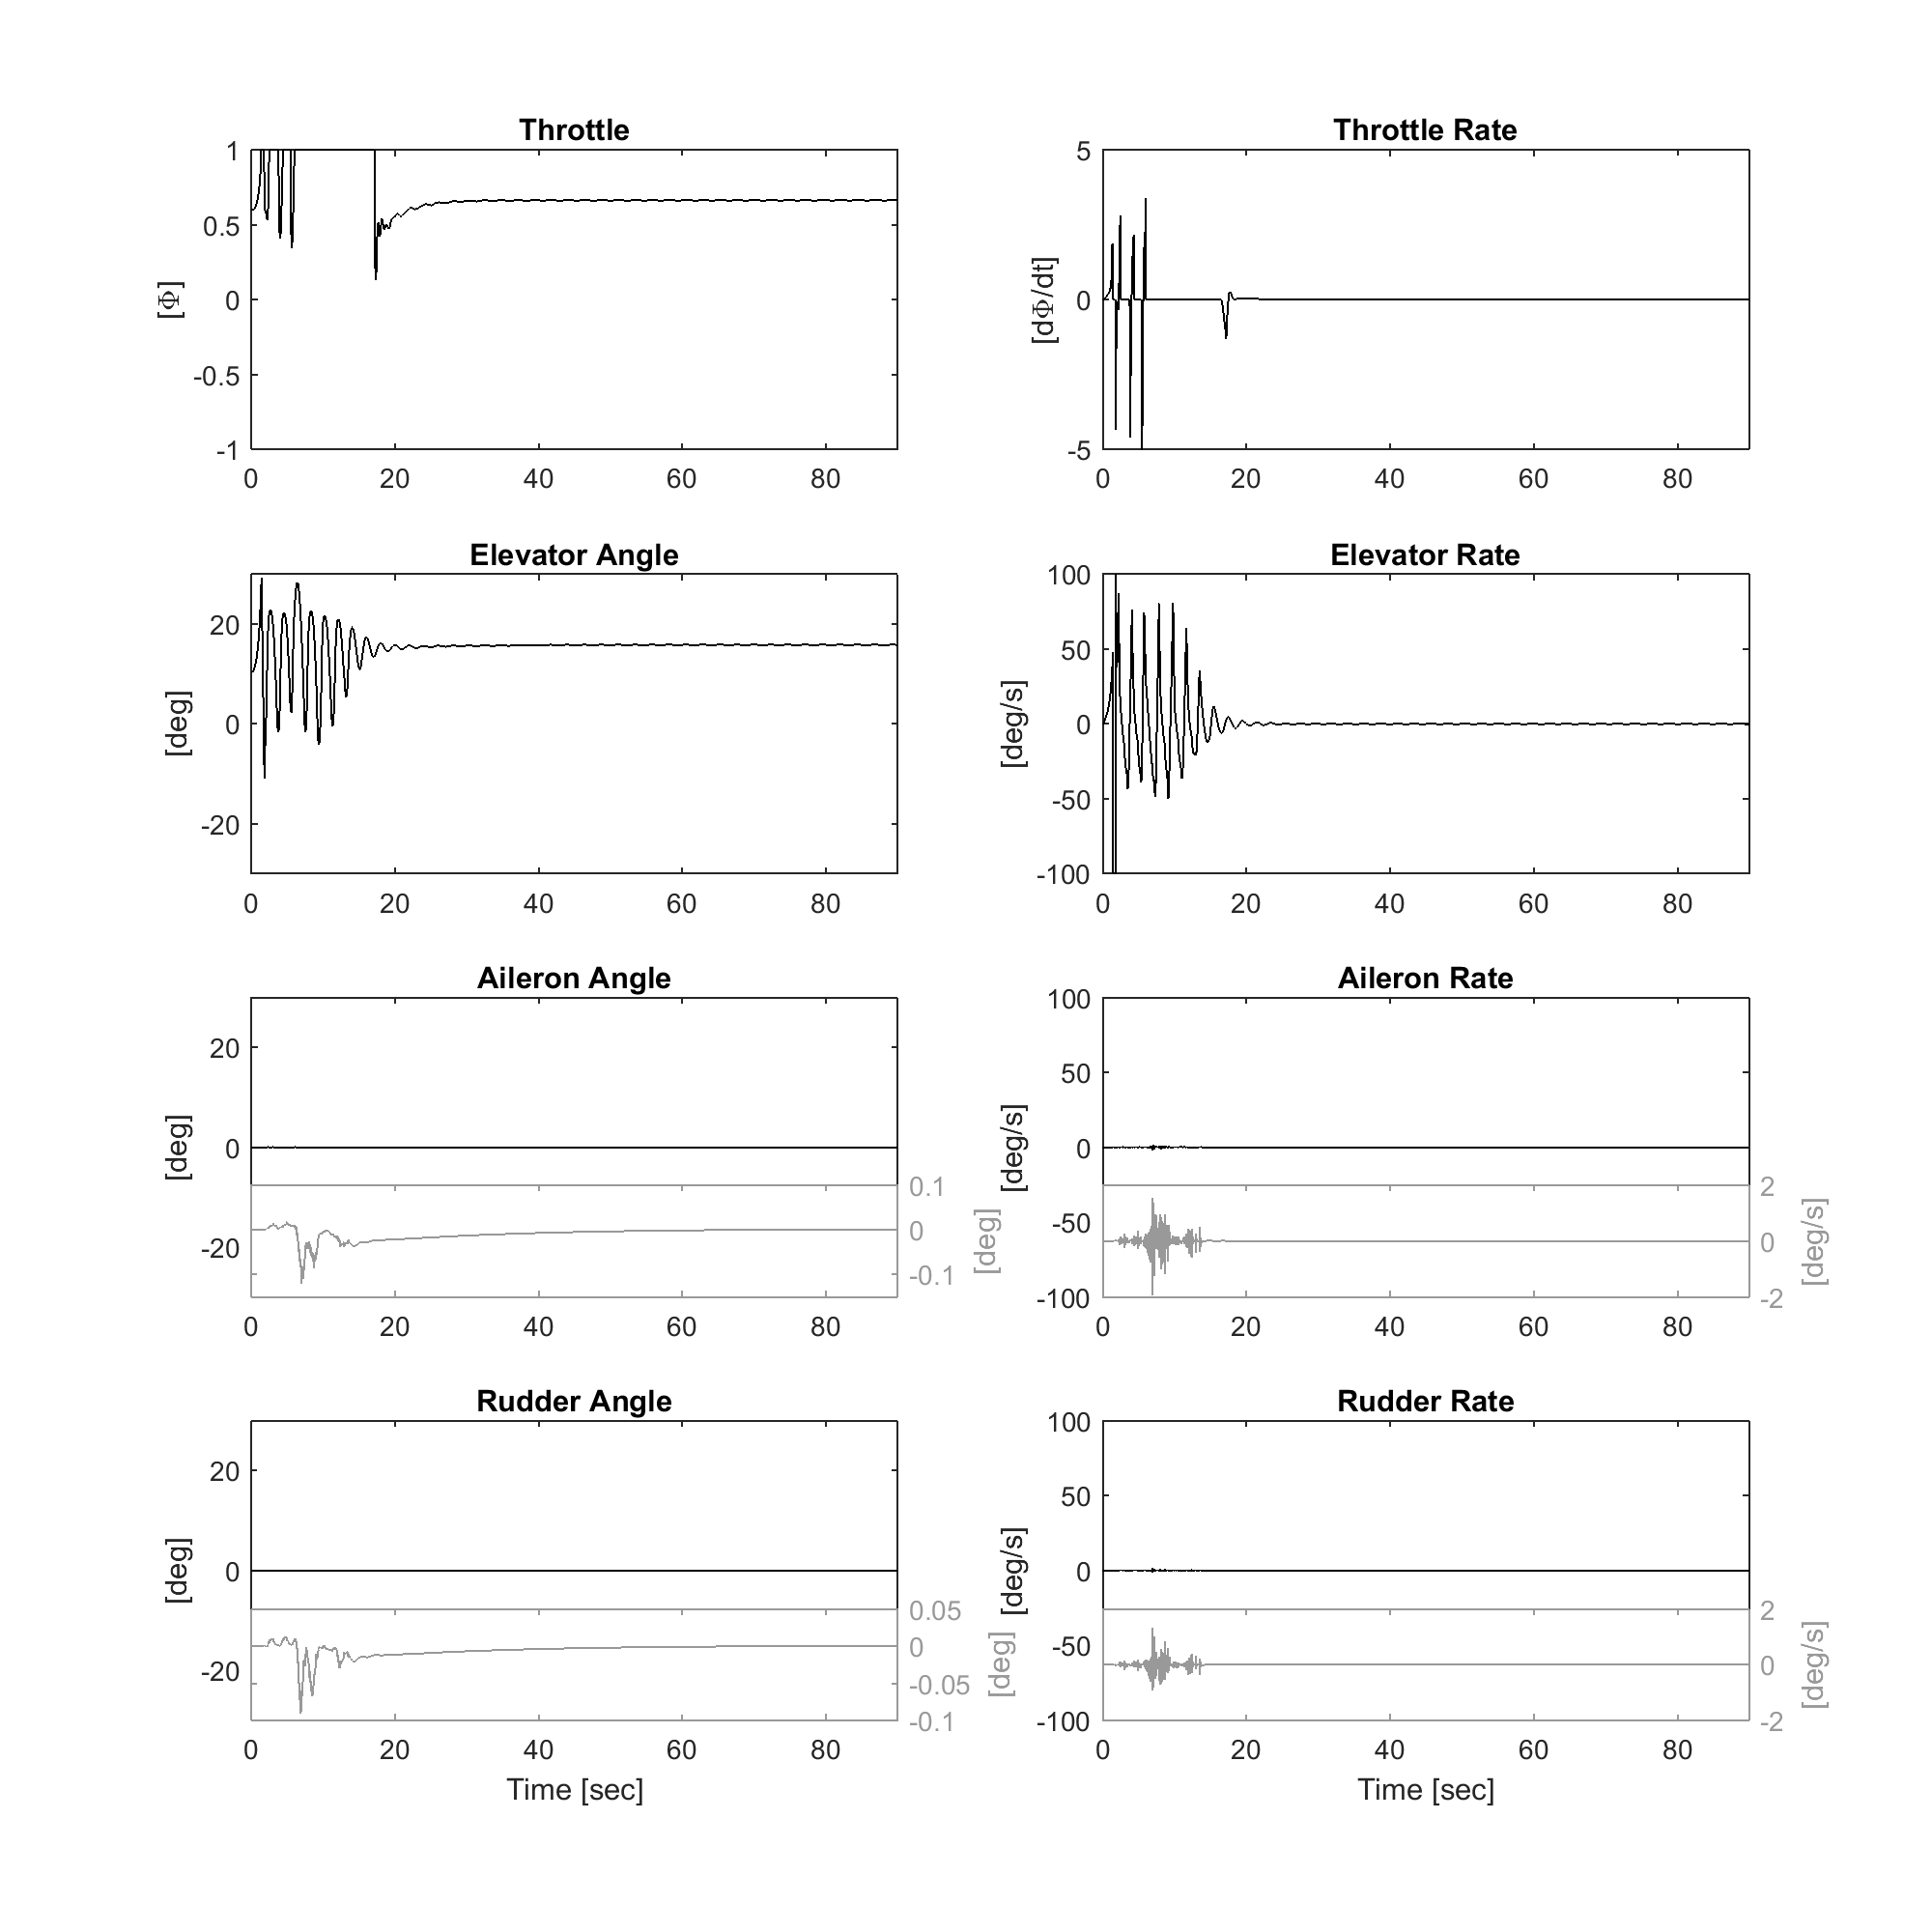
\includegraphics[width=7.5in]{\figurepath/adaptiveUncertainLongControl.png}}
  \vspace{-1.0in}
  \caption{Plant control input for adaptive controller applied to uncertain plant in response to a 1000 ft.\ climb command.\label{fig.adaptiveUncertainLongControl}}
\end{figure}

\newpage
\begin{figure}[H]
  \hspace{-0.5in}
  \noindent\makebox[7.5in]{%
  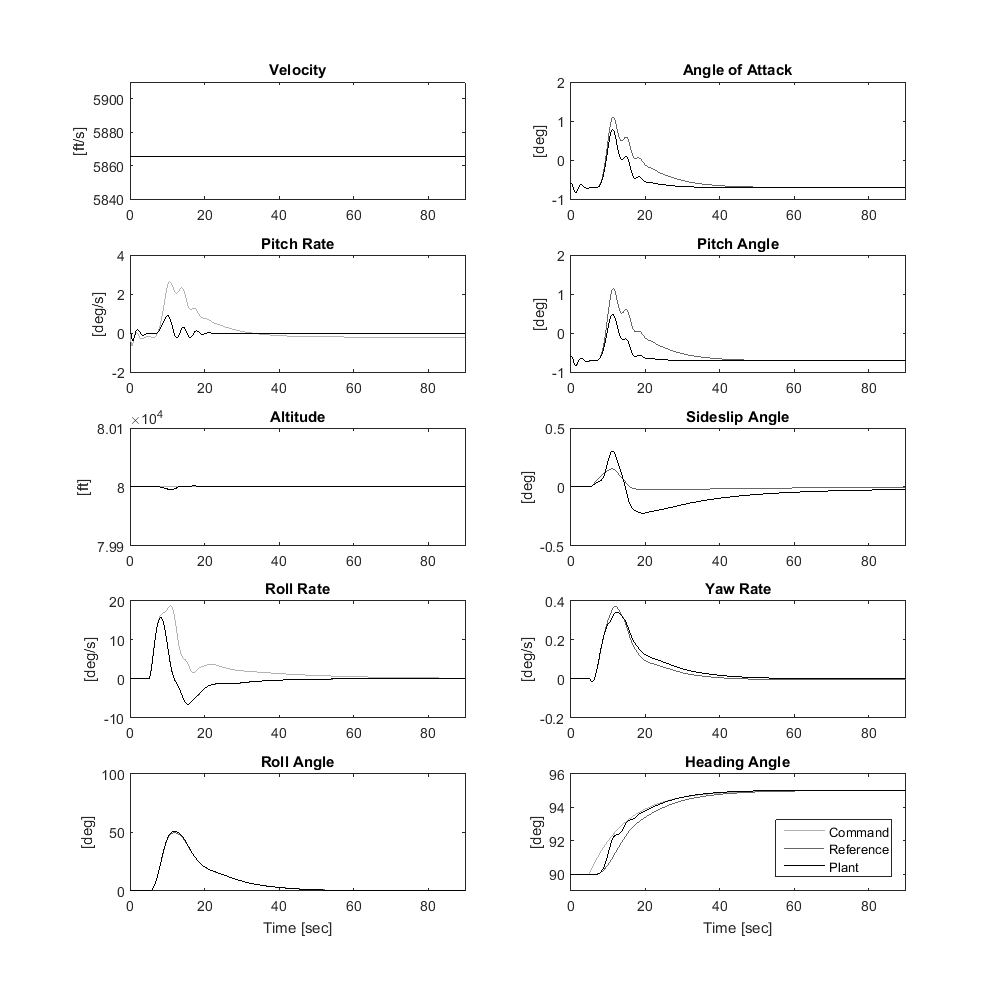
\includegraphics[width=7.5in]{\figurepath/baselineNominalLatrState.png}}
  \vspace{-1.0in}
  \caption{Plant states for baseline controller applied to nominal plant in response to a 5 degree heading turn.\label{fig.baselineNominalLatrState}}
\end{figure}

\newpage
\begin{figure}[H]
  \hspace{-0.5in}
  \noindent\makebox[7.5in]{%
  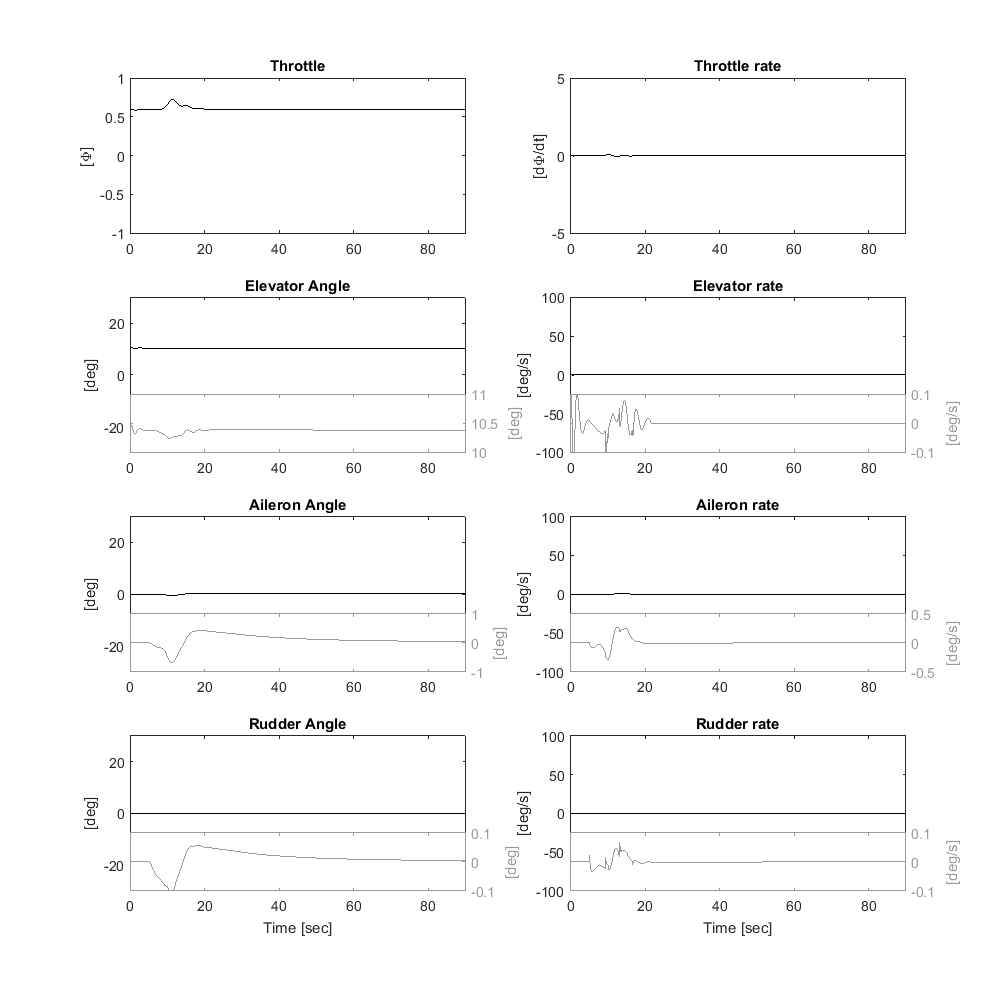
\includegraphics[width=7.5in]{\figurepath/baselineNominalLatrControl.png}}
  \vspace{-1.0in}
  \caption{Plant control input for baseline controller applied to nominal plant in response to a 5 degree heading turn.\label{fig.baselineNominalLatrControl}}
\end{figure}

\newpage
\begin{figure}[H]
  \hspace{-0.5in}
  \noindent\makebox[7.5in]{%
  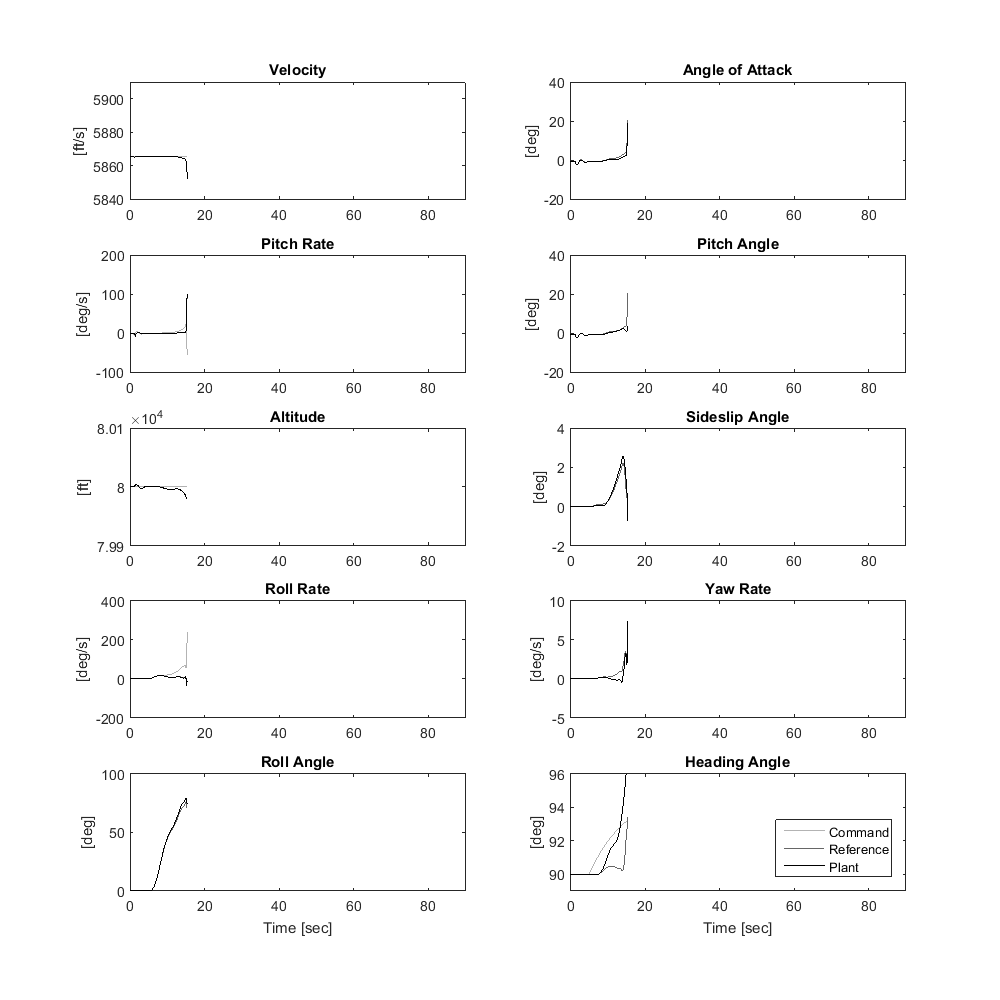
\includegraphics[width=7.5in]{\figurepath/baselineUncertainLatrState.png}}
  \vspace{-1.0in}
  \caption{Plant states for baseline controller applied to uncertain plant in response to a 5 degree heading turn.\label{fig.baselineUncertainLatrState}}
\end{figure}

\newpage
\begin{figure}[H]
  \hspace{-0.5in}
  \noindent\makebox[7.5in]{%
  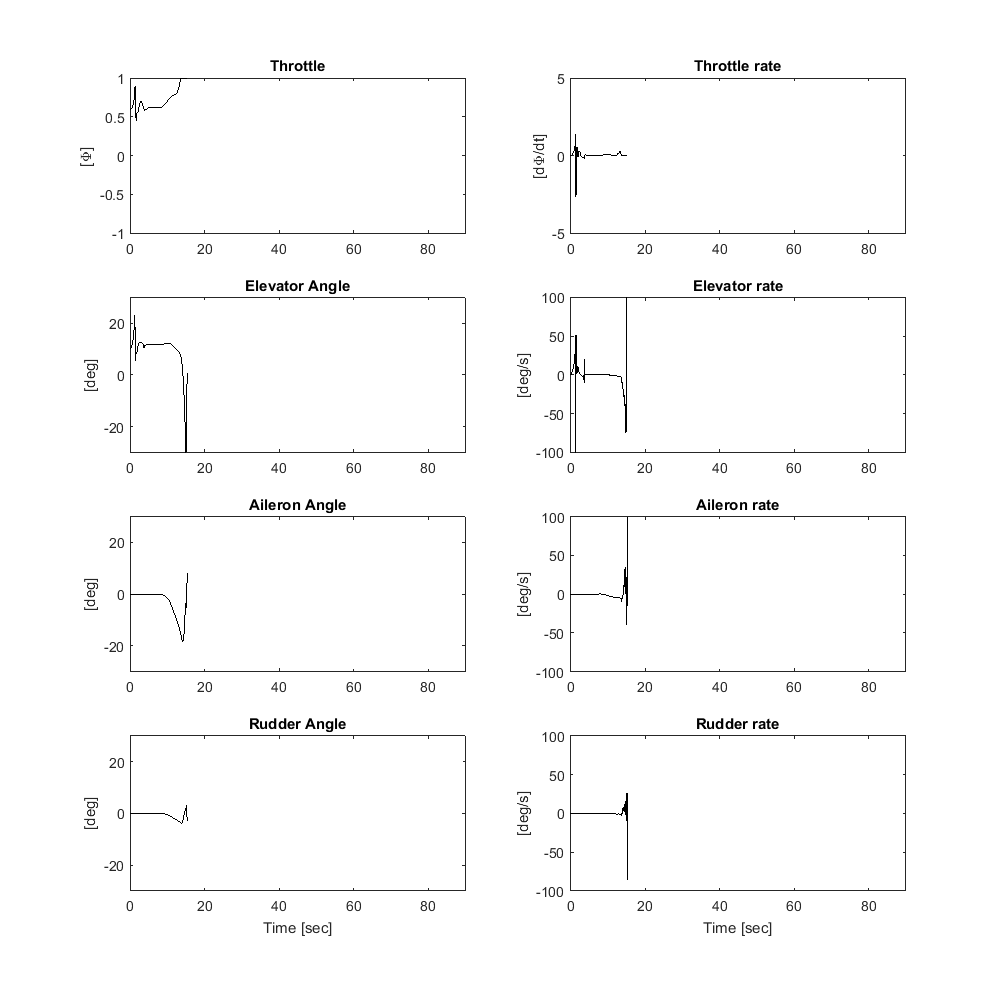
\includegraphics[width=7.5in]{\figurepath/baselineUncertainLatrControl.png}}
  \vspace{-1.0in}
  \caption{Plant control input for baseline controller applied to uncertain plant in response to a 5 degree heading turn.\label{fig.baselineUncertainLatrControl}}
\end{figure}

\newpage
\begin{figure}[H]
  \hspace{-0.5in}
  \noindent\makebox[7.5in]{%
  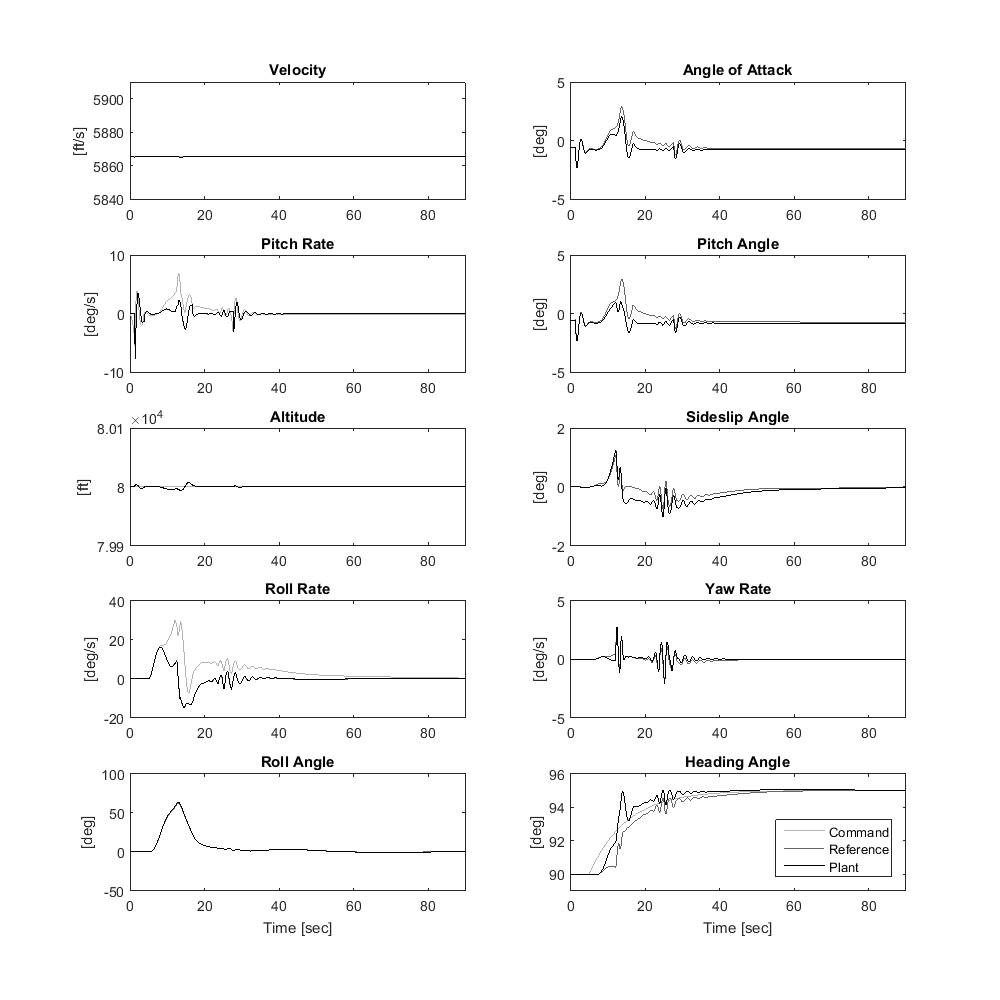
\includegraphics[width=7.5in]{\figurepath/adaptiveUncertainLatrState.png}}
  \vspace{-1.0in}
  \caption{Plant states for adaptive controller applied to uncertain plant in response to a 5 degree heading turn.\label{fig.adaptiveUncertainLatrState}}
\end{figure}

\newpage
\begin{figure}[H]
  \hspace{-0.5in}
  \noindent\makebox[7.5in]{%
  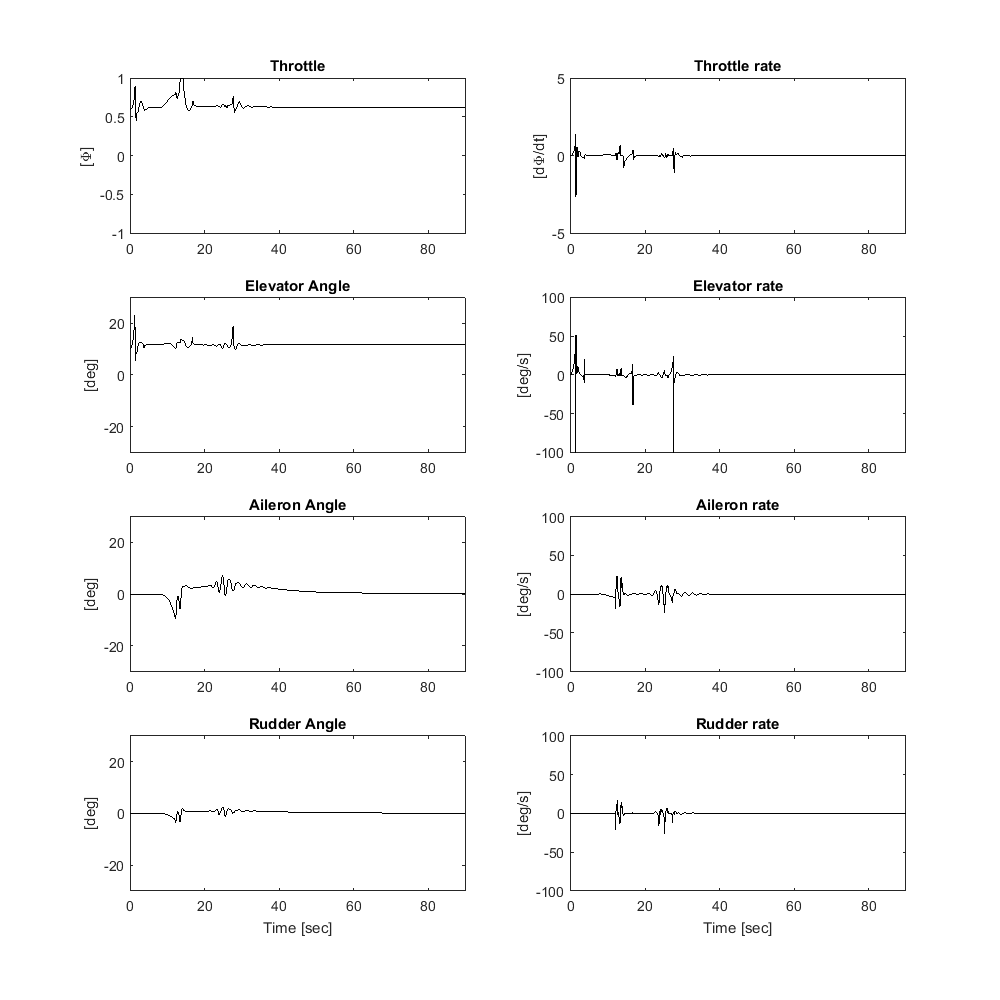
\includegraphics[width=7.5in]{\figurepath/adaptiveUncertainLatrControl.png}}
  \vspace{-1.0in}
  \caption{Plant control input for adaptive controller applied to uncertain plant in response to a 5 degree heading turn.\label{fig.adaptiveUncertainLatrControl}}
\end{figure}

\subsection{Outer-loop Response with Limiter}

The outer-loop responses in Sec.~\ref{sec.numericalExample.outerLoop} showed the ability of the combined inner and outer-loop controller to provide good command tracking of the outer-loop heading and altitude commands, while maintaining stability in the presence of uncertainty when the baseline controller could not.
However, despite stability and good command tracking performance, in Figs.~\ref{fig.adaptiveUncertainLatrState} and~\ref{fig.adaptiveUncertainLatrControl}, for example, there are significant oscillations present in the response, and large deviations in sideslip.
On the GHV such large deviations in sideslip angle would likely lead to unstart and further instability, although this phenomenon was not captured in the nonlinear GHV model used for the simulations in this thesis.
Regardless, it is beneficial to be able to suppress these large sideslip angle deviations, and ensure coordinated flight is maintained.
It is for this purposed that the limiter described in Sec.~\ref{sec.outerLoop.stateLimiting} is used.

Figs.~\ref{fig.stateLimiterState} and~\ref{fig.stateLimiterControl} show the same response as in Figs.~\ref{fig.adaptiveUncertainLatrState} and~\ref{fig.adaptiveUncertainLatrControl}, with the exception of the addition of the state limiter.
The modulation function is selected so as $\gamma=0$ for $\beta\in[-0.1,\;0.1]$ deg, and $\gamma=1$ for $\beta\notin[-0.2,\;0.2]$.
These regions, defined by the sets $\Omega_{\delta}$ and $\Omega$, are plotted in the figure.
Corollary~\ref{cor.notForcingLimiting} is easily verified, to ensure that for the given heading angle command that asymptotic tracking will be achieved.
This agrees with intuition, as it is expected that at the completion of a turn to a new heading, that the aircraft should be in coordinated flight, with zero sideslip angle.
Furthermore, by enforcing coordinated flight throughout the turn, Figs.~\ref{fig.adaptiveUncertainLatrState} and~\ref{fig.adaptiveUncertainLatrControl} show the drastically reduced oscillations observed in Figs.~\ref{fig.stateLimiterState} and~\ref{fig.stateLimiterControl}.

To further illustrate the effect that the limiter has on the inner and outer-loop commands, Fig.~\ref{fig.comparison} shows a comparison between the inner and outer-loop commands from the response without the limiter, shown in Fig.~\ref{fig.adaptiveUncertainLatrState}, to those with the limiter, shown in Fig.~\ref{fig.stateLimiterState}.
When not using the limiter, the outer-loop command is equal to the desired value, that is $z_{g,\text{cmd}}(t)=z_{g,\text{cmd}}^{\prime}(t)$, and the inner-loop input is also equal to the command value as $r(t)=r_{\text{cmd}}(t)$.
When using the limiter, the command $z_{g,\text{cmd}}(t)$ and $r(t)$ are modified from the desired or commanded values, as shown.
The limiting of both of these inner and outer-loop command signals is what is used to limit the sideslip angle, also shown in Fig.~\ref{fig.comparison}.
Because the outer-loop command $z_{g,\text{cmd}}(t)$ is used to generate the inner-loop command $r_{\text{cmd}}(t)$, the outer-loop limiting has an indirect effect on the inner-loop command.
However, the inner-loop command is further limited, resulting in $r(t)$ as shown.
It is the limiting of these commands that is responsible for the improved time response demonstrated in the simulations

From Corollary~\ref{cor.notForcingLimiting}, another situation that may be encountered, is one where for piecewise constant commands $\|z_{g,\text{cmd}}^{\prime}(t)\|_{\infty}>z_{g,\text{cmd,max}}^{\prime}$, in which case asymptotic tracking of the command is not obtained.
Consider, for example, applying the state limiter to enforce a limit on the roll angle, so as to limit the G-loading during a turn.
Figs.~\ref{fig.stateLimiterRollAngleState} and~\ref{fig.stateLimiterRollAngleControl} show the state limiter used in this way to limit the roll angle to 20 degrees.
However, by limiting the bank angle during a turn, the turn rate of the aircraft is limited.
To make large heading angle changes, large bank angles are required.
With the roll angle limiter becoming invoked simply as a result of the command, asymptotic command tracking does not follow.

\newpage
\begin{figure}[H]
  \hspace{-0.5in}
  \noindent\makebox[7.5in]{%
  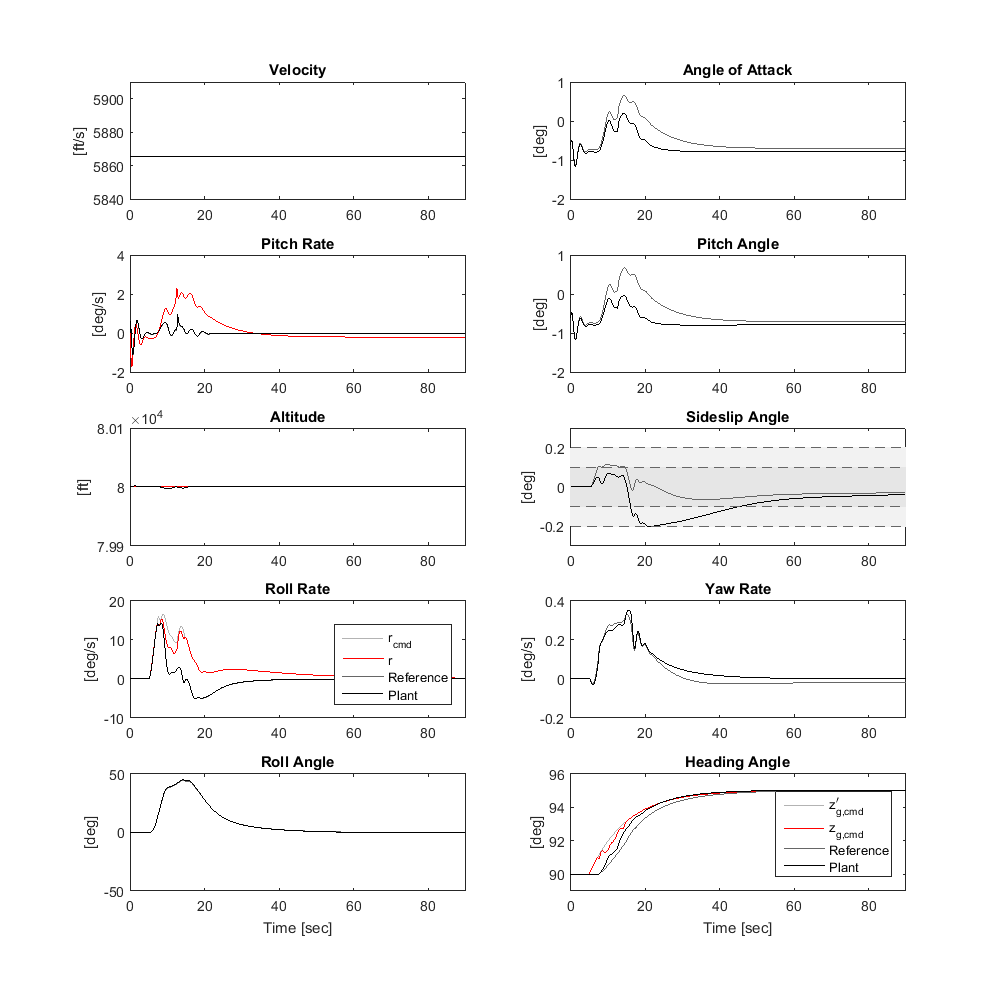
\includegraphics[width=7.5in]{\figurepath/adaptiveStateLimiterLatr2State.png}}
  \vspace{-1.0in}
  \caption{Plant states for adaptive controller applied to uncertain plant in response to a 5 degree heading turn with sideslip angle Limiter.\label{fig.stateLimiterState}}
\end{figure}

\newpage
\begin{figure}[H]
  \hspace{-0.5in}
  \noindent\makebox[7.5in]{%
  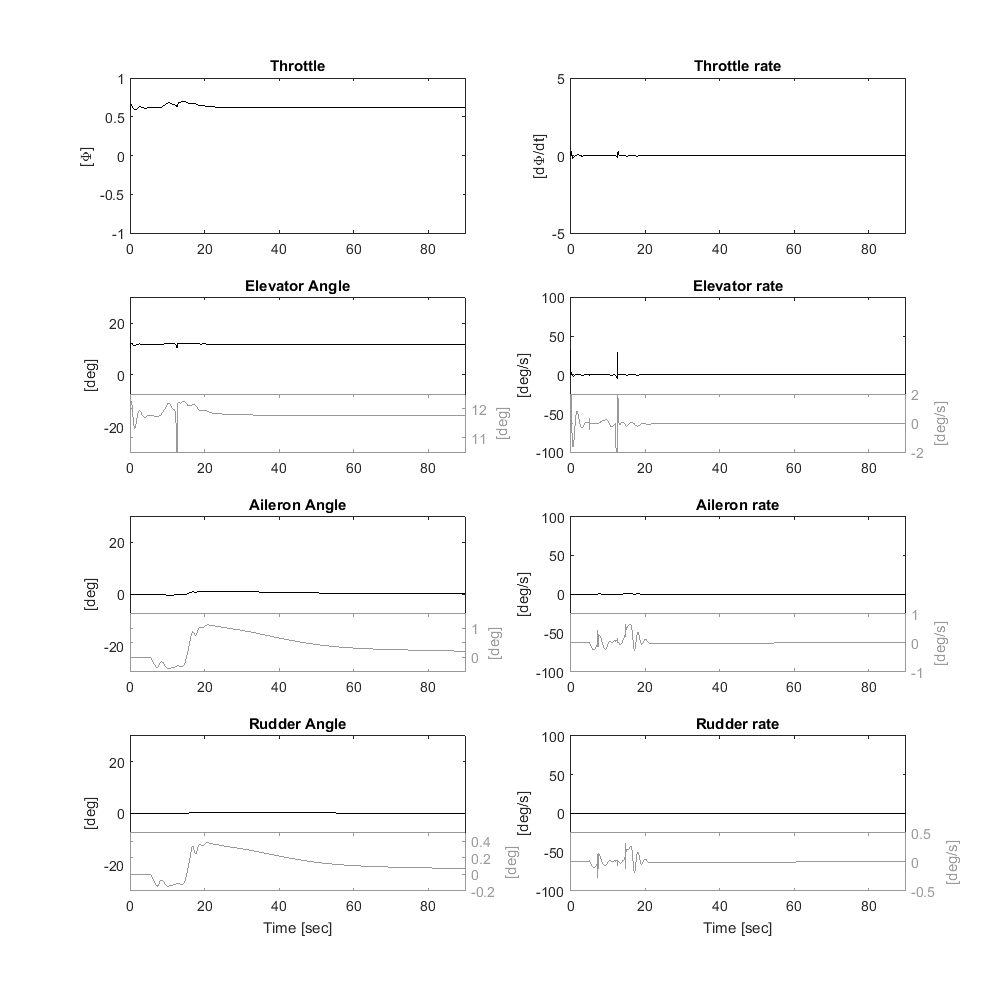
\includegraphics[width=7.5in]{\figurepath/adaptiveStateLimiterLatr2Control.png}}
  \vspace{-1.0in}
  \caption{Plant control input for adaptive controller applied to uncertain plant in response to a 5 degree heading turn with sideslip angle Limiter.\label{fig.stateLimiterControl}}
\end{figure}

\newpage
\begin{figure}[H]
  \hspace{-0.5in}
  \noindent\makebox[7.5in]{%
  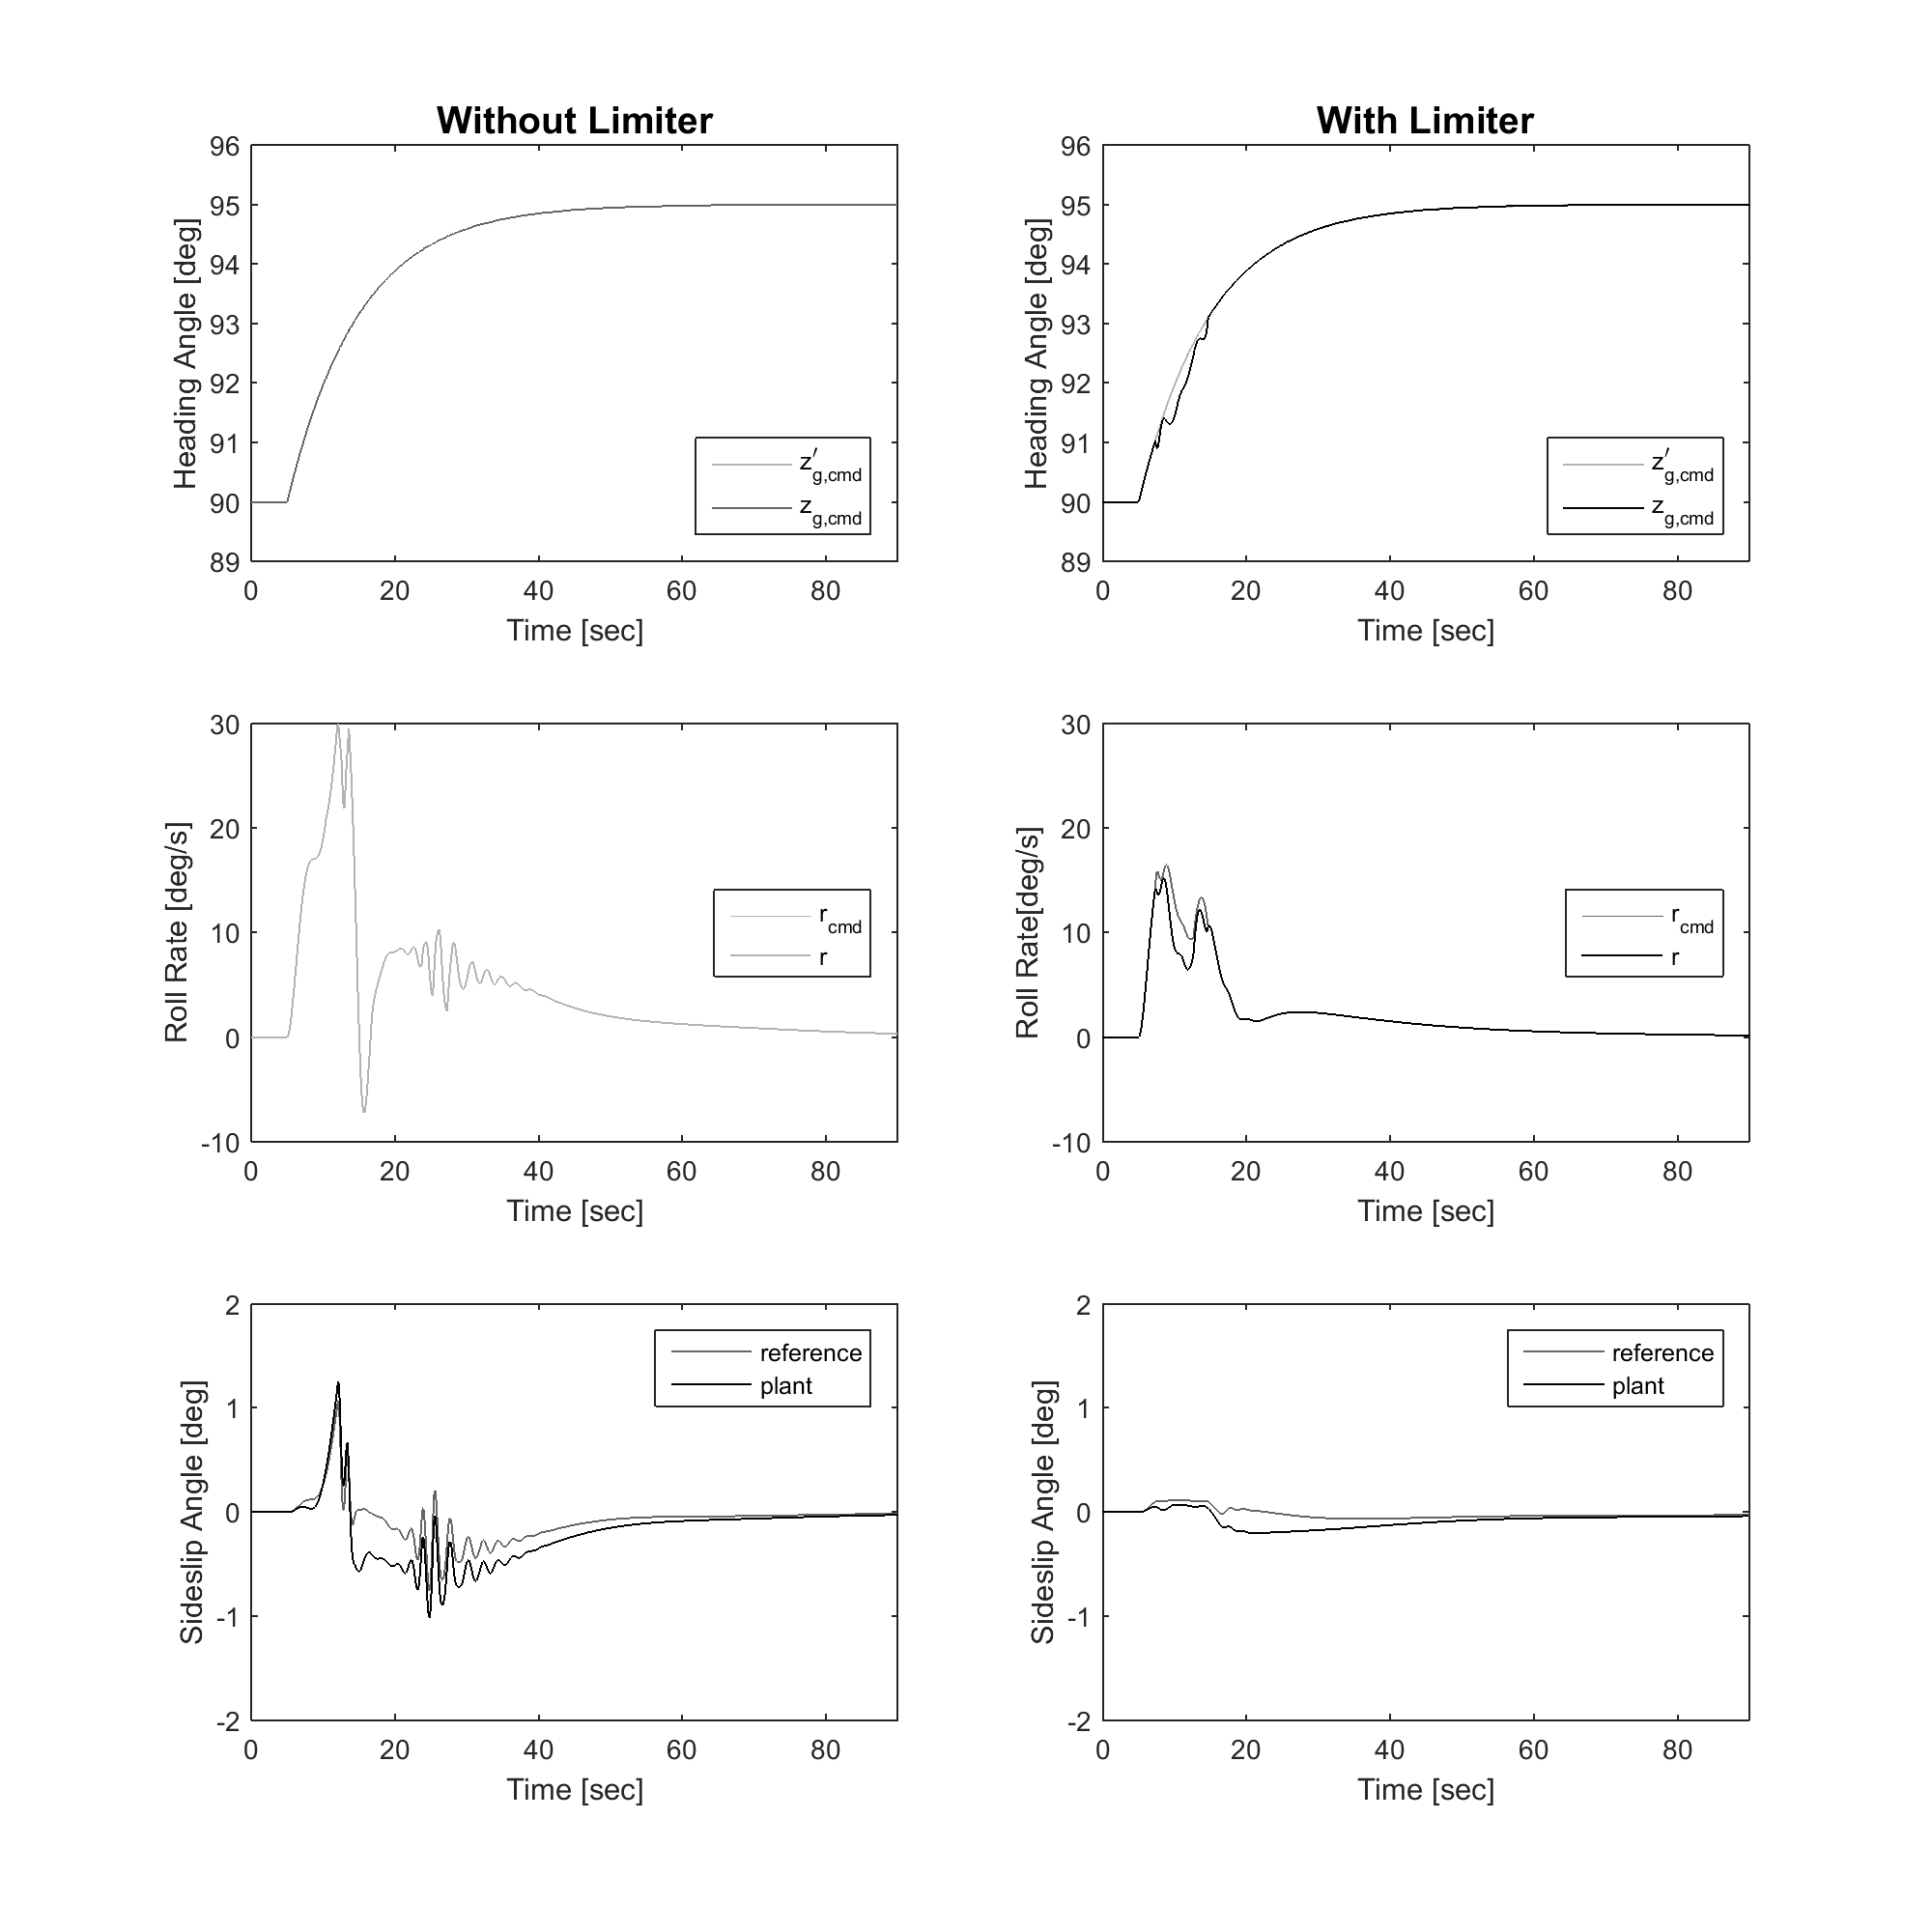
\includegraphics[width=7.5in]{\figurepath/comparison2.png}}
  \vspace{-1.0in}
  \caption{Comparison between inner and outer-loop commands when using the limiter to limit sideslip angle.\label{fig.comparison}}
\end{figure}

\newpage
\begin{figure}[H]
  \hspace{-0.5in}
  \noindent\makebox[7.5in]{%
  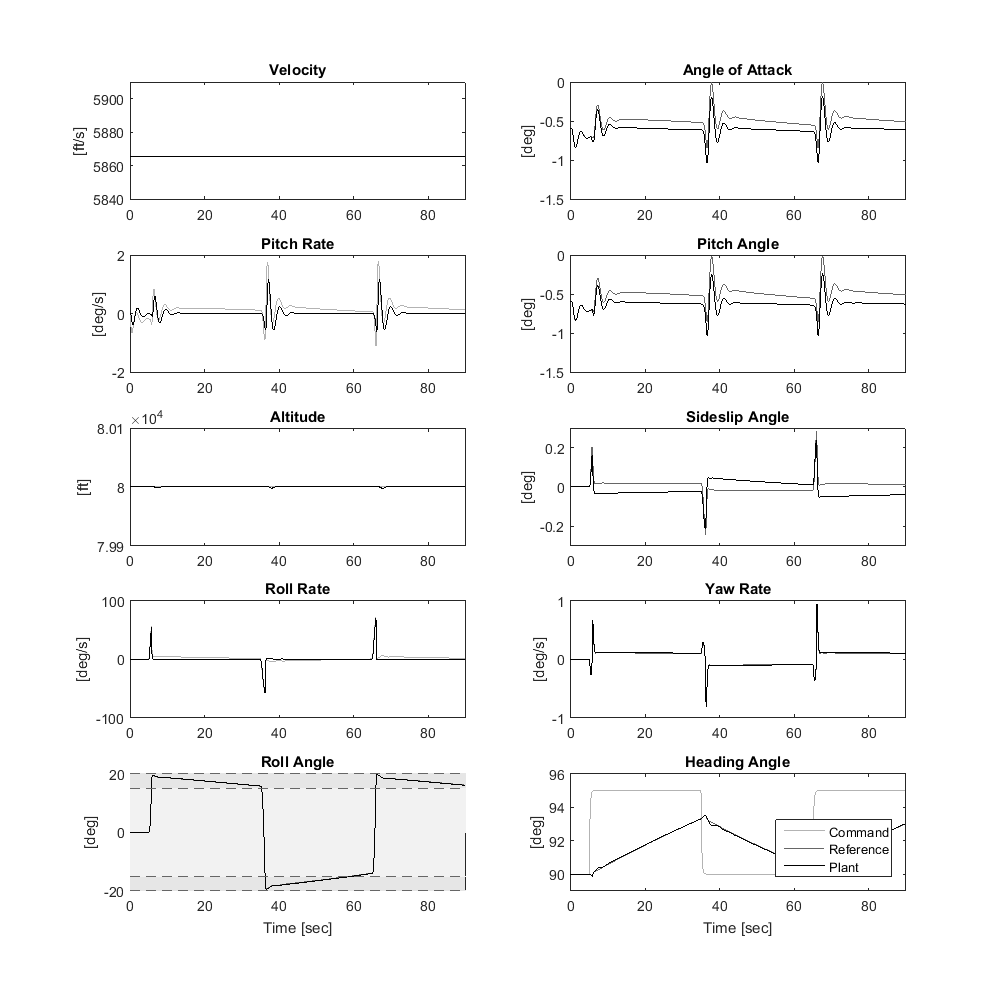
\includegraphics[width=7.5in]{\figurepath/baselineStateLimiterLatrRollAngleState.png}}
  \vspace{-1.0in}
  \caption{Plant states for adaptive controller applied to uncertain plant in response to a 5 degree heading turn with roll angle Limiter.\label{fig.stateLimiterRollAngleState}}
\end{figure}

\newpage
\begin{figure}[H]
  \hspace{-0.5in}
  \noindent\makebox[7.5in]{%
  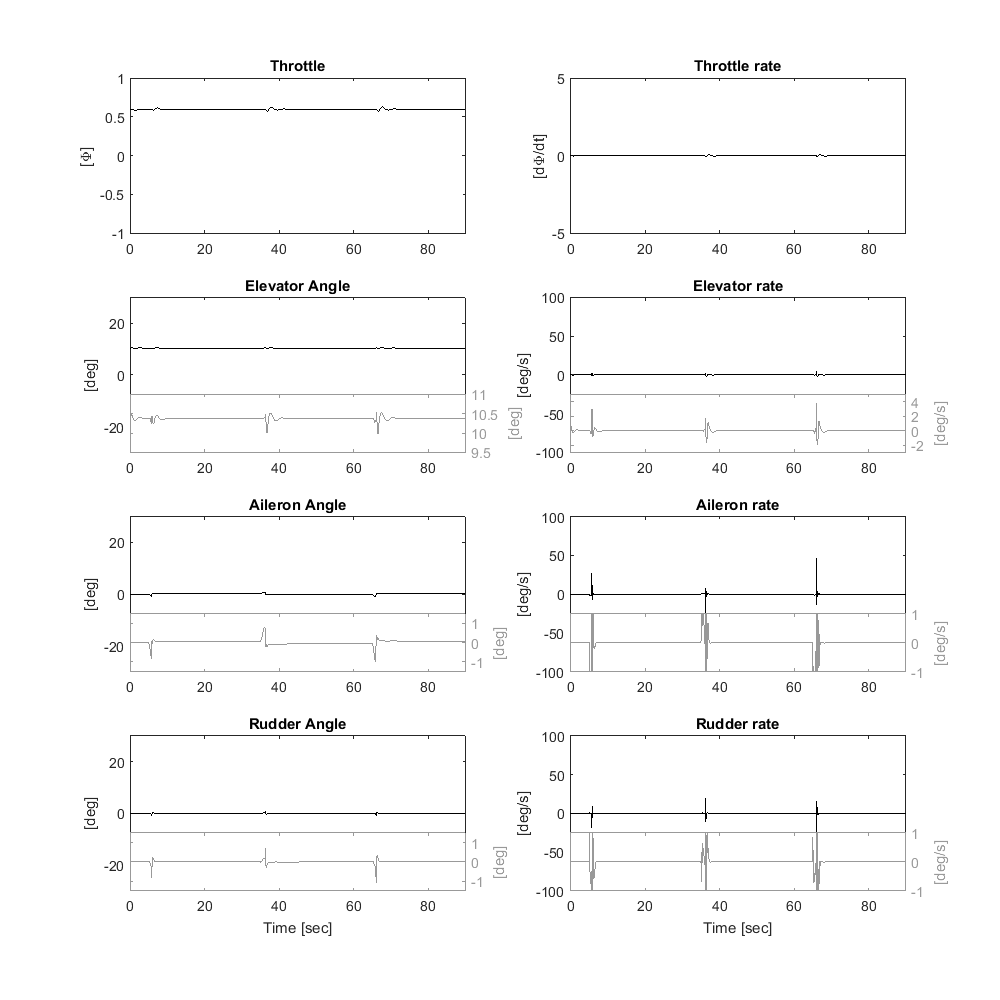
\includegraphics[width=7.5in]{\figurepath/baselineStateLimiterLatrRollAngleControl.png}}
  \vspace{-1.0in}
  \caption{Plant control input for adaptive controller applied to uncertain plant in response to a 5 degree heading turn with roll angle Limiter.\label{fig.stateLimiterRollAngleControl}}
\end{figure}
